\chapter{深度里兹法求解椭圆多特征值问题}
椭圆方程的特征值问题在数学、物理学和工程学中有着广泛的应用。 例如，在量子力学中，薛定谔方程描述了量子系统的行为，其解的特征值对应于系统的能级。 在结构力学中，特征值问题用于分析结构的振动模式和稳定性。 传统的数值方法，如有限元法和谱方法，已经被广泛应用于求解椭圆方程的特征值问题。然而，这些方法在处理高维问题或复杂几何形状时可能面临计算成本高和精度不足的挑战。

\section{预备知识与记号}
\subsection{问题背景与物理意义}
椭圆型特征值问题在数学物理中占据核心地位，其理论根植于对自然界基本波动现象的描述。在宏观尺度上，经典的薄膜振动模型（如鼓面振动）提供了最直观的物理背景。设鼓面位移为 $U(x, t)$，其运动遵循波动方程 $U_{tt} = c^2 \Delta U$。若寻求驻波解（Standing Wave），即通过分离变量法设 $U(x, t) = u(x) \cos(\omega t)$，则空间分布函数 $u(x)$ 满足如下亥姆霍兹（Helmholtz）方程：
\begin{equation}
-\Delta u = \lambda u
\end{equation}
此处，特征值 $\lambda = (\omega/c)^2$ 直接关联系统的振动频率，而特征函数 $u$ 则刻画了振动的本征模态（Eigenmode）。

特征值谱不仅决定了系统的动力学行为，更内蕴了定义域 $\Omega$ 的几何拓扑信息。这一联系引出了著名的等谱问题（Isospectral Problem）：即马克·卡克（Mark Kac）提出的“能否通过听鼓声测出鼓面的形状？”。从数学角度看，这意味着特征值的分布与区域几何特征存在深刻对偶。外尔定律（Weyl's Law）精确地量化了这一关系：特征值的渐近增长率由区域的体积决定。对于二维区域 $\Omega$，特征值 $\lambda_n$ 表现出如下谱渐近行为：
$$\lambda_n \sim \frac{4\pi n}{\text{Area}(\Omega)} \quad (n \to \infty)$$
这一深刻结论表明，通过分析频谱特征，可以反演重构出物体的体积、表面积乃至曲率等几何不变量，该理论在现代遥感成像及逆问题研究中具有基础性意义。

在微观尺度上，椭圆型特征值问题同样构成了量子力学的基石。描述微观粒子运动的定态薛定谔方程：
$$-\frac{\hbar^2}{2m}\Delta \psi + V\psi = E\psi$$
本质上即为带有势能项 $V$ 的椭圆型特征值问题。式中，特征值 $E$ 对应系统容许的量子化能级，特征函数 $\psi$ 则描述粒子在空间出现的概率幅。由此可见，有界区域上椭圆算子谱的离散性，正是量子力学中能量量子化现象的数学根源。

综上所述，无论是在宏观声学还是微观量子力学中，椭圆型特征值问题都是描述物理系统稳态的关键数学模型。

\subsection{数学描述和谱定理}
基于上述物理背景，我们将问题抽象为一般形式的数学模型。本文主要研究如下带有Dirichlet边界条件的椭圆型特征值问题：
\begin{equation}\label{eq:eigendiriproblem}
\left\{\begin{aligned}
-\Delta u(x)+V(x) u(x) &=\lambda u(x) & & \text { in } \Omega \\
T u(x) &=0 & & \text { on } \partial \Omega,
\end{aligned}\right.
\end{equation}

其中~$\Omega \subset \mathbb{R}^{d}$~是一个非空的有界闭集, 其边界 $\partial \Omega$ 满足适当的光滑性假设。$V\in L^{\infty}(\Omega): \Omega \rightarrow \mathbb{R}$~是给定的势函数, $T$~是边界迹算子。特征值问题要求对应的$(\lambda, u)$对，满足上述的椭圆方程。不失一般性，我们假设势函数 $V$ 满足一致正下界条件，即存在常数 $c_0 > 0$，使得 $V(x) \ge c_0$ 在 $\Omega$ 上几乎处处成立。

根据椭圆偏微分方程的经典理论\cite{evans2010partial}，上述微分算子 $\mathcal{L} = -\Delta + V$ 在配备 Dirichlet 边界条件的 Hilbert 空间 $L^2(\Omega)$ 上是自伴的，且由于区域 $\Omega$ 的有界性，其逆算子（或格林算子）$\mathcal{L}^{-1}$ 是紧算子。这一性质使得我们可以直接应用泛函分析中的紧自伴算子谱定理：

\begin{theorem}[谱分解定理]
设 $\mathcal{H}$ 为可分希尔伯特空间，若 $\mathcal{K}: \mathcal{H} \to \mathcal{H}$ 为紧自伴算子，则：
\begin{enumerate}
    \item $\mathcal{H}$ 中存在由 $\mathcal{K}$ 的特征向量 $\{u_n\}_{n=1}^{\infty}$ 构成的完备正交基。
    \item 任意函数 $f \in \mathcal{H}$ 均可按该基底展开为广义傅里叶级数：
    $$ f = \sum_{n=1}^{\infty} \langle f, u_n \rangle u_n $$
    其中 $\langle \cdot, \cdot \rangle$ 表示 $\mathcal{H}$ 中的内积。
\end{enumerate}
\end{theorem}

基于谱定理，方程\eqref{eq:eigendiriproblem}的特征值与特征函数具有如下基本性质：

\begin{lemma}\label{lemma:eigen_properties}
对于椭圆型特征值问题\eqref{eq:eigendiriproblem}，结论如下成立：
\begin{enumerate}
    \item {\heiti 实谱性}：所有特征值 $\lambda$ 均为实数。
    \item {\heiti 离散性与排序}：特征值构成一个可列的离散集合，且仅以 $+\infty$ 为聚点。若考虑代数重数，特征值可按非递减顺序排列为：
    \begin{equation}\label{eq:eigenvalue_sequence}
    0 < \lambda_{1} < \lambda_{2} \leq \lambda_{3} \leq \cdots, \quad \text{且 } \lim_{k \to \infty} \lambda_{k} = +\infty.
    \end{equation}
    \item {\heiti 完备正交性}：对应的特征函数系 $\{\xi_{k}\}_{k=1}^{\infty}$ 构成 $L^{2}(\Omega)$ 空间的一组完备正交基。
\end{enumerate}
\end{lemma}

为简化后续推导，本文约定特征函数系 $\{\xi_{k}\}_{k=1}^{\infty}$ 已关于 $L^{2}$ 范数进行归一化，即 $\|\xi_{k}\|_{L^{2}(\Omega)}=1$。


\subsection{符号约定与正则性假设}

为叙述简便，本节统一规定文中使用的符号与定义。

\begin{definition}[基础符号与算子]\label{def:notation}
\quad
\begin{enumerate}
    \item {\heiti 内积与范数}：记 $\langle\cdot,\cdot\rangle$ 为 $L^{2}(\Omega)$ 空间的标准内积，$\|\cdot\|$ 为对应的 $L^{2}$ 范数。
    
    \item {\heiti 谱投影算子}：基于算子 $\mathcal{L}$ 的特征值分解，定义谱投影算子 $\mathcal{P}_{<k}$ 为：
    \begin{equation*}
        \mathcal{P}_{<k}u = \sum_{\lambda_{l}<\lambda_{k}} \langle u,\xi_{l} \rangle \xi_{l}.
    \end{equation*}
    即 $\mathcal{P}_{<k}$ 表示将函数 $u$ 投影至由特征值（严格）小于 $\lambda_k$ 的特征向量所生成的子空间。类似地，我们可以定义 $\mathcal{P}_{>k}$, $\mathcal{P}_{=k}$, $\mathcal{P}_{\leq k}$, $\mathcal{P}_{\geq k}$ 以及 $\mathcal{P}_{\neq k}$。
    
    \item {\heiti 特征值分离度}：定义特征值 $\lambda_i$ 的分离度为：
    \begin{equation*}
        \delta \lambda_{i} = \min_{j: \lambda_{j}\neq \lambda_{i}} |\lambda_{i}-\lambda_{j}|.
    \end{equation*}
    
    \item {\heiti 渐近符号}：在不等式估计中，使用符号 $A \lesssim B$ 表示存在一个与关键参数无关的有界常数 $C$，使得 $A \leq CB$。若常数依赖于特定参数，将特别注明。
    
    \item {\heiti 辅助函数}：定义 $\varphi(x) = x\log(x)$ ($x>1$)，并记 $\psi(x)$ 为 $\varphi(x)$ 的反函数。
\end{enumerate}
\end{definition}

\begin{remark}
对于上述定义的函数 $\psi(x)$，易证对于任意 $0<k<1$，成立 $\psi(kx) \geq k\psi(x)$。此外，该函数满足如下渐近性质：
$$ \forall \alpha>0, \quad \varphi(x) \lesssim x^{1+\alpha}, \quad \psi(x) \gtrsim x^{1-\alpha}. $$
\end{remark}

关于谱投影算子，基于紧自伴算子的谱理论可知，由于 $\mathcal{P}_{<k}$ 是由特征基底构成的投影，它在 $L^{2}$ 内积和能量内积（即与椭圆算子关联的双线性形式）下均是正交投影。
需要特别注意的是，由于特征值可能存在重数（Multiplicity），即特征空间的维数可能大于 1，上述定义中不同的索引 $k$ 可能对应相同的特征值。这也是我们在公式 \eqref{eq:eigenvalue_sequence} 中使用非严格不等号 ($\leq$) 的原因。

特征值问题的正则性（Regularity）是本文分析的另一个核心要素。足够高的正则性对于避免高维问题中的“维数灾难”（Curse of Dimensionality）至关重要（详见第 \ref{sec_main} 节）。为此，我们提出如下假设：

\begin{assumption}[正则性假设]\label{ass:regularity}
假设区域 $\Omega$ 和势函数 $V$ 满足：
\begin{enumerate}
    \item[(a)] $\Omega \subset \mathbb{R}^d$ 是一个有界的 $C^{m}$ 区域；
    \item[(b)] 势函数 $V \in C^{m-1}(\bar{\Omega})$；
    \item[(c)] $m > \max\{2, \frac{d}{2}-2\}$。
\end{enumerate}
\end{assumption}

上述关于区域边界的正则性假设主要是为了满足 Whitney 延拓定理的条件，该定理在第 \ref{subsec_app} 节的误差分析中起到了关键作用。
值得指出的是，虽然本文的理论推导基于上述光滑性假设，但结论通常可以推广到更广泛的几何情形。例如，$\mathbb{R}^{d}$ 中的单位立方体虽然在角点处不满足 $C^m$ 边界条件，但若势函数为常数或齐次势，我们的定理结论显然依然成立。针对此类非光滑区域的有效性，我们将在第 \ref{sec_num} 节通过数值算例进一步验证。

\section{模型构建}
\subsection{特征值与瑞利商}
针对前文公式 \eqref{eq:eigendiriproblem} 定义的椭圆型特征值问题，其变分形式自然对应于瑞利商（Rayleigh Quotient）的极值问题。为此，我们首先定义如下的双线性能量泛函：

\begin{equation*}
a(u,v)\triangleq\langle \nabla u,\nabla v\rangle+\int_{\Omega}w uv \text{d}x, u\in H_{0}^{1}(\Omega).
\end{equation*}

而瑞利商则定义为：
\begin{equation*}
R(u) = \frac{a(u,u)}{\langle u, u \rangle}
\end{equation*}

基于瑞利-里兹变分原理，椭圆算子的基态特征值$\lambda_1$ 可通过在容许函数空间内极小化瑞利商（Rayleigh Quotient）来刻画。具体而言，$\lambda_1$ 及其对应的特征函数 $\xi_1$ 满足：
\begin{equation}\label{eq:first_eigen}
\lambda_1 = \min_{\substack{u \in H_0^1(\Omega) \ u \neq 0}} \frac{a(u,u)}{\langle u, u \rangle}, \quad \xi_1 \in \mathop{\arg\min}_{\substack{u \in H_0^1(\Omega) \ u \neq 0}} \frac{a(u,u)}{\langle u, u \rangle}.
\end{equation}

对于高阶特征值，我们可以采用递归变分法进行定义。第 $k$ 个特征值 $\lambda_k$ 对应于瑞利商在与前 $k-1$ 个特征特征函数正交的子空间上的最小值。即：
\begin{equation}\label{eq:ktheigenvalue}
\lambda_k = \min_{\substack{u \in H_0^1(\Omega), u \neq 0 \\ \langle u,\xi_j\rangle=0, 1 \le j < k}} \frac{a(u,u)}{\langle u, u \rangle}, \quad \xi_k \in \mathop{\arg\min}_{\substack{u \in H_0^1(\Omega), u \neq 0 \\ \langle u,\xi_j\rangle=0, 1 \le j < k}} \frac{a(u,u)}{\langle u, u \rangle}.
\end{equation}

虽然理论上我们可以直接基于经典的深度里兹法，利用公式 \eqref{eq:ktheigenvalue} 来求解第 $k$ 个特征值及其对应的特征函数，但在实际计算中，该方法的直接应用面临着以下三个主要的本质困难：

\begin{itemize}
\item 第一个困难在于如何确保神经网络近似解满足 Dirichlet 零边界条件。从函数空间的角度审视，标准神经网络生成的函数空间 $\mathcal{N}$ 通常仅满足 $\mathcal{N} \subset H^{1}(\Omega)$，而非 $\mathcal{N} \subset H^{1}_{0}(\Omega)$。
虽然部分现有工作（如 \cite{lu2021priorieigen}）尝试通过构造距离函数或特殊网络结构来“硬约束”边界条件，但这类方法往往局限于规则区域，难以推广至复杂几何形状，且增加了理论分析的难度。
针对一般区域的 PDE 问题，边界惩罚法（Boundary Penalty Method）提供了一种更为灵活的“软约束”策略 \cite{duan2021analysis, Mller2021ErrorEF}。其核心思想是引入如下修正的双线性形式：
\begin{equation}\label{eq:penalty_bilinear}
a^{\mu_1}(u,v) = a(u,v) + \mu_1\int_{\partial \Omega}uv \text{d}s,
  \end{equation}
其中 $\mu_1 > 0$ 为惩罚项参数。实际上，罚函数形式\ref{eq:penalty_bilinear}严格对应于如下 Robin 边值问题的变分形式：
\begin{equation*}
\left\{\begin{aligned}
-\Delta u + V u &= \lambda u & \text{ in } \Omega, \\
\frac{1}{\mu_1}\frac{\partial u}{\partial n} + u &= 0 & \text{ on } \partial\Omega.
\end{aligned}\right.
\end{equation*}
本文将严格证明：当 $\mu_1 \to +\infty$ 时，上述 Robin 问题的特征对将收敛于原 Dirichlet 问题的特征对。因此，本文提出的框架天然适用于一般的 Robin 特征值问题。为叙述简便，后文在不引起混淆的情况下将不再刻意区分两者。

\item 第二个困难源于瑞利商泛函本身的几何性质。瑞利商具有尺度不变性（零次齐次性），即对于任意非零常数 $c$，有 $R(c u) = R(u)$。这意味着优化目标在特征函数的径向方向上是常数，导致解空间呈现出流形结构而非单一极小值点，极大地削弱了梯度的导向性。
更为严重的是，这种非凸性导致优化过程在原点附近极不稳定。当近似解的模长趋于零（$\|v\| \to 0$）时，瑞利商的梯度计算将出现奇异性，导致优化问题变得病态（Ill-posed）。为克服这一平凡解风险，必须在损失函数中引入适当的正则化项或稳定项（Stabilizer）\cite{Weinan2017The}，以约束解的模长并维持数值稳定性。

\item 求解高阶特征值（$k > 1$）面临着额外的正交性难题。根据变分原理（Min-Max Principle），能量泛函的无约束最小化总是倾向于收敛至基态（最小特征值 $\lambda_1$）。为了捕获第 $k$ 个激发态，必须强制当前的近似解与前 $k-1$ 个已求得的特征函数保持正交。
在深度学习框架下，这种正交性通常通过在损失函数中添加罚项来实现。然而，这不仅引入了额外的超参数，还使得优化图景变得更加崎岖，增加了陷入局部极小值或发生模式塌缩的风险。
\end{itemize}

\subsection{损失函数及其稳定性估计}
为了克服上述挑战，本文并未采用直接优化瑞利商的传统策略，而是构造了如下的损失函数作为变分目标。基于该目标函数，我们建立了如下定理：

\begin{theorem}\label{th:3.1}
记 $Q(v)=\|v\|^{2}-1$。定义第 $k$ 个特征值的损失函数为：
\begin{equation}\label{eq:conloss}
\mathcal{L}_{k}(v)=\frac{1}{2}a^{\mu_{1}}(v,v)+\frac{\mu_{2}}{4}\left[Q(v)^{2}+2\sum_{i<k}\left\langle v,\frac{\xi_{i}}{\|\xi_{i}\|}\right\rangle^{2}\right],
\end{equation}
设 $\xi_{k}$ 为该损失函数在空间 $H^1$ 中的极小值点，即：
\begin{equation*}
\xi_{k}\in \mathop{\text{argmin}}_{v\in H^{1}}\ \mathcal{L}_{k}(v).
\end{equation*}
若惩罚参数满足 $\mu_{2}>2\lambda_{k}$，并记$\varepsilon_1=\frac{1}{\mu_1}$，则如下误差估计成立：
\begin{equation*}
0<\lambda_{k}-\frac{a^{\mu_{1}}(\xi_{k},\xi_{k})}{\langle \xi_{k},\xi_{k}\rangle}\lesssim C(\Omega,w)\varepsilon_1.
\end{equation*}
此外，在忽略 $a^{\mu_{1}}$ 特征空间内线性变换（即相差一个特征子空间内的旋转或常数因子）的意义下，$\xi_{k}$ 是 $\mathcal{L}_{k}$ 的唯一极小化子。
\end{theorem}

\begin{proof}
不失一般性，我们可以假设所有 $\xi_{k}$ 均已归一化。
证明主要包含两个步骤：
首先，我们将证明当惩罚参数 $\mu_1 \to +\infty$ 时，如下 Robin 边值问题的特征对收敛于 Dirichlet 问题的特征对（其中 $T$ 表示迹算子）：
\begin{equation}\label{eq:eigenrobinproblem}
\left\{\begin{aligned}
-\Delta u+w u &=\lambda^{\mu_{1}} u & & \text { in } \Omega, \\
\left(T + \frac{1}{\mu_{1}}\frac{\partial}{\partial n}\right) u &=0 & & \text { on } \partial \Omega.
\end{aligned}\right.
\end{equation}

具体而言，其特征值$\lambda^{\mu_1}$和Dirichlet问题的特征值$\lambda$满足如下误差估计：
\begin{equation*}
0<\lambda-\lambda^{\mu_{1}}\lesssim C(\Omega,w)\frac{1}{\mu_{1}},
\end{equation*}

随后，我们将证明损失函数 $\mathcal{L}_k$ 的极小化项 $\xi_{k}$ 恰为Robin边值问题 \eqref{eq:eigenrobinproblem} 的特征向量。

我首先给出第一部分的证明。为此，我们定义算子 $A: L^{2}(\Omega) \to L^{2}(\Omega)$为 Dirichlet 边值问题的源项到解的映射，即：
\begin{equation}\label{eq:Adef2}
\left\{\begin{aligned}
(-\Delta+w) Af &= f & &\text{in } \Omega, \\
TAf &= 0 & &\text{on } \partial\Omega.
\end{aligned}\right.
\end{equation}

对于式\eqref{eq:Adef2}，若区域 $\Omega$ 是 $C^2$ 区域或凸多边形，则有椭圆方程的先验估计
\begin{equation}\label{eq:prior}
\|Af\|_{H^2(\Omega)} \lesssim \|f\|_{L^2(\Omega)}.
\end{equation}

以及迹定理成立：
\begin{equation}\label{eq:trace}
\|\frac{\partial }{\partial n}Af\|_{H^{1/2}(\partial \Omega)} \lesssim \|TAf\|_{H^{3/2}(\partial \Omega)} \lesssim \|Af\|_{H^2(\Omega)}.\\
\end{equation}

类似地，定义 $A^{\mu_{1}}: L^{2}(\Omega) \to L^{2}(\Omega)$ 为 Robin 边值问题的源项到解的映射，即：
\begin{equation}\label{eq:Adef}
\left\{\begin{aligned}
(-\Delta+w) A^{\mu_{1}}f &= f & &\text{in } \Omega, \\
\left(T+\frac{1}{\mu_{1}}\frac{\partial }{\partial n}\right)A^{\mu_{1}}f &= 0 & &\text{on } \partial\Omega,
\end{aligned}\right.
\end{equation}

其对应的先验估计和迹定理同样成立。

文献 \cite{Maury2009Numerical}（命题 2.3 的证明）已确立了 $A^{\mu_{1}}$ 强收敛于 $A$ 这一结论。尽管该结果对于求解椭圆方程已足够，但尚不足以直接证明特征值问题的收敛性。我们需要证明对于一列特征值序列$\{\xi_k\}_{k=1}^{\infty}$，都有$A^{\mu_1}\xi_k$在 $H^1(\Omega)$ 中收敛于 $A\xi_k$。因此，需要将进一步证明 $A^{\mu_{1}}$ 在算子范数意义下收敛于 $A$。

我们首先沿用 \cite{Maury2009Numerical} 中的方法建立 $A^{\mu_{1}}$ 的强收敛性，该估计为应用一致有界原理提供了必要的一致有界性条件。为此，我们定义如下的残差泛函：

%TODO 把引用写成引理

%Lemma (Elliptic Regularity on Convex Domains):Let $\Omega \subset \mathbb{R}^2$ be a bounded convex polygonal domain. Assume $f \in L^2(\Omega)$. Then the unique solution $u \in H^1_0(\Omega)$ to the Dirichlet problem $-\Delta u = f$ satisfies $u \in H^2(\Omega)$, and there exists a constant $C$ independent of $u$ such that:
% $$\|u\|_{H^2(\Omega)} \leq C \|f\|_{L^2(\Omega)}.$$
% Proof Reference: This result is a direct consequence of the regularity theory for polygonal domains, specifically established by Kadlec (1964) and detailed in Grisvard (1985, Theorem 3.2.1.2).

% Grisvard (最权威的引用):

% Grisvard, P. (1985). Elliptic Problems in Nonsmooth Domains. Pitman. (特别是第3章)

% Kadlec (原始证明):

% Kadlec, J. (1964). The regularity of the solution of the Poisson problem in a domain whose boundary is similar to that of a convex domain. Czechoslovak Mathematical Journal, 14(3), 386-393.

\begin{equation}\label{eq:R_lambda}
R^{\mu_{1}}(v) = \frac{1}{2}a^{\mu_{1}}( Af-v , Af-v )+\frac{\mu_{1}}{2}\int_{\partial\Omega}\left( -\frac{1}{\mu_{1}}\frac{\partial Af}{\partial n}-v \right)^{2} \text{d}s.
\end{equation}

由式\eqref{eq:prior}和式\eqref{eq:trace}，法向导数 $\frac{\partial }{\partial n}Af, \frac{\partial }{\partial n}A^{\mu_{1}}f\in H^{1/2}(\partial \Omega)$, 而$H^{1/2}(\partial \Omega)$ 是紧嵌入到 $L^2(\partial \Omega)$, 因此法向导数$\frac{\partial }{\partial n}Af, \frac{\partial }{\partial n}A^{\mu_{1}}f$ 是平方可积的。故上述定义的泛函 $R^{\mu_{1}}$ 是良定义的。

利用方程 \eqref{eq:Adef}，泛函 \eqref{eq:R_lambda} 可重写为：
\begin{equation*}
\begin{aligned}
R^{\mu_{1}}(v) &= \frac{1}{2}a^{\mu_{1}}( Af,Af) - a^{\mu_{1}}( Af,v) +\frac{1}{2}a^{\mu_{1}}( v,v ) \\
&\quad +\frac{1}{2\mu_{1}}\int_{\partial\Omega}\left(\frac{\partial Af}{\partial n}\right)^{2}ds +\int_{\partial\Omega}\frac{\partial Af}{\partial n}vds+\frac{\mu_{1}}{2}\int_{\partial\Omega}v^{2}ds \\
&= \frac{1}{2}a^{\mu_{1}}( Af,Af)+\frac{1}{2}a^{\mu_{1}}( v,v )-\langle f,v\rangle \\
&\quad +\frac{1}{2\mu_{1}}\int_{\partial\Omega}\left(\frac{\partial Af}{\partial n}\right)^{2}ds +\frac{\mu_{1}}{2}\int_{\partial\Omega}v^{2}ds.
\end{aligned}
\end{equation*}

% 上式的推导表明，$A^{\mu_{1}}f$ 正是泛函 $R^{\mu_{1}}$ 的极小化项。根据逆迹定理，存在一个有界的延拓算子，使得$\frac{\partial Af}{\partial n}$在$\Omega$上的延拓有界，取测试函数$v = Af - \frac{1}{\mu_1}T^{-1}\frac{\partial Af}{\partial n}$，我们有如下估计：
上式的推导表明，$A^{\mu_{1}}f$ 正是泛函 $R^{\mu_{1}}$ 的极小化项。我们构造如下的测试函数$v = Af - \frac{1}{\mu_1}\frac{\partial Af}{\partial n}$并带入$R(u)$中，我们得到如下估计：
\begin{equation*}
\begin{aligned}
R^{\mu_{1}}(A^{\mu_{1}}f) &\leq R^{\mu_{1}}\left(Af-T^{-1}\frac{1}{\mu_{1}}\frac{\partial Af}{\partial n}\right)\\
&= \frac{1}{2\mu_{1}^{2}}a^{\mu_{1}}\left(T^{-1}\frac{\partial Af}{\partial n}, T^{-1}\frac{\partial Af}{\partial n}\right) \\
&\leq C\mu_{1}^{-2}.
\end{aligned}
\end{equation*}

由 $a^{\mu_{1}}(\cdot,\cdot)$ 的椭圆性，可得：
\begin{equation*}
R^{\mu_{1}}(A^{\mu_{1}}f-Af)\geq C_1\|A^{\mu_{1}}f-Af\|_{H^{1}(\Omega)}^{2},
\end{equation*}

从而：
\begin{equation*}
\|(A-A^{\mu_{1}})f\|_{H^{1}(\Omega)}\leq C\mu_{1}^{-1},
\end{equation*}

从而我们证明了 $A^{\mu_{1}}$ 强收敛于 $A$，且由一致有界原理，该算子序列的估计是一致有界的（$C$不依赖于$\mu_{1}$和$f$），从而证明了特征函数的收敛性。进一步，为了得到特征值的误差估计，我们考察如下二次型的误差估计：
\begin{equation*}
\begin{aligned}
\langle A^{\mu_{1}}f, f\rangle - \langle Af, f\rangle &= \langle A^{\mu_{1}}f, (-\Delta+w) Af\rangle - \langle Af, f\rangle \\
&= \langle (-\Delta+w)A^{\mu_{1}}f, Af\rangle - \langle Af, f\rangle \\
&\quad + \int_{\partial \Omega} \frac{\partial}{\partial n} A^{\mu_{1}}f \cdot T Af \, ds - \int_{\partial \Omega} T A^{\mu_{1}}f \cdot \frac{\partial}{\partial n} Af \, ds \\
&= \frac{1}{\mu_{1}}\int_{\partial \Omega} \frac{\partial }{\partial n}A^{\mu_{1}}f \cdot \frac{\partial }{\partial n}Af \, ds \\
&= \frac{1}{2\mu_{1}}\left(
\left\|\frac{\partial}{\partial n}A^{\mu_{1}}f\right\|_{L^{2}}^{2} + \left\|\frac{\partial}{\partial n}Af\right\|_{L^{2}}^{2} - \left\|\frac{\partial}{\partial n}(A^{\mu_{1}}-A)f\right\|_{L^{2}}^{2}
\right).
\end{aligned}
\end{equation*}

而前文由式\eqref{eq:prior}和\eqref{eq:trace}已推知$\frac{\partial }{\partial n}Af, \frac{\partial }{\partial n}A^{\mu_{1}}f$在$L^2(\partial\Omega)$中可积，因此
\begin{equation*}
|\lambda^{\mu_1} - \lambda| \le \sup_{\|f\|=1} | \langle (A^{\mu_1} - A)f, f \rangle |\le C\mu_{1}^{-1}.
\end{equation*}

从而完成了第一部分的证明。

下面进行证明的第二部分。为记号简便起见，我们将省略 $A^{\mu_1}$（原为 $A$）及其特征值、特征向量和特征分解的具体依赖标记。我们采用数学归纳法进行证明。为便于叙述，在讨论 $\mathcal{L}_k$ 时，假设对于所有 $i<k$，$\xi_i$ 均已归一化。由公式 \eqref{eq:conloss}，$\mathcal{L}_{k}$ 的变分形式可表示为:
\begin{equation*}
\left.\delta \mathcal{L}_{k}\right(u;\delta u)=a^{\mu_1}(u,\delta u)+\mu_1\left[Q(u) \langle \delta u, u\rangle+ \sum\limits_{i<k}\langle \delta u,\xi_{i} \rangle\langle \xi_{i},u \rangle\right].
\end{equation*}

首先考虑 $k = 1$ 的情形。令 $\delta \mathcal{L}_{1}(\xi_1)=0$，可导出 \begin{equation}\label{eq:3.16}
\left\{
\begin{aligned}
\left[-\Delta+w+\mu_2Q(\xi_{1})\right]\xi_{1}&=0,\\
\left(\frac{1}{\mu_1}\frac{\partial}{\partial n}+T\right)\xi_{1}&=0.
\end{aligned}
\right.
\end{equation}

这表明 $\xi_{1}=\vec{0}$，或者 $\xi_{1}$ 是对应于特征值 $-\mu_{2}Q(\xi_{1})$ 的特征向量；记该特征值为 $\lambda_{l_{1}}$。由于 $Q(v)=\|v\|^{2}-1\geq -1$，可知 $\lambda_{l_{1}}\leq \mu_{2}$。因此，根据正交性，若 $\mu_{2}>\lambda_{1}$，则至少存在一个非平凡驻点。此时二阶变分公式为：

\begin{equation*}
\begin{aligned}
\delta^{2} \mathcal{L}_{k}(u;\delta u)=& \frac{1}{2}a^{\mu_{1}}(\delta u,\delta u) +\frac{\mu_{2}}{2}\left[2\langle u, \delta u\rangle^{2}+Q(\xi_{k})\|\delta u\|^{2}+\sum_{i<k}\left\langle\xi_{i}, \delta u\right\rangle^{2}\right].
\end{aligned}
\end{equation*}

若 $l_{1}=1$，即 $\xi_{1}$ 是对应于主特征值 $\lambda_{1}$ 的特征向量，满足 $\|\xi_{1}\|^2=1-\frac{\lambda_{1}}{\mu_{2}}$。此时我们可以证明：
$$\begin{aligned}
\delta^{2} \mathcal{L}_{1}(\xi_1;\mathcal{P}_{>1}\delta u)
&=\frac{1}{2}a^{\mu_{1}}(\mathcal{P}_{>1}\delta u,\mathcal{P}_{>1}\delta u)+\frac{\mu_{2}}{2}\left[2\langle\xi_1, \mathcal{P}_{>1}\delta u\rangle^{2}+Q(\xi_{1})|\mathcal{P}_{>1}\delta u|^{2}\right]\\
&\geq\frac{1}{2}\lambda_{2}|\mathcal{P}_{>1}\delta u|^{2}+\frac{\mu_{2}}{2}\left(-\frac{\lambda_{1}}{\mu_{2}}|\mathcal{P}_{>1}\delta u|^{2}\right)\\
&\geq\frac{1}{2}\delta\lambda_{1}|\mathcal{P}_{>1}\delta u|^{2}>0,
\end{aligned}$$

注意到 $\mathcal{P}_{\leq 1}\delta u$ 满足 Eq.~\eqref{eq:3.16}，我们有：
\begin{equation}\label{eq:3.20}
\delta^{2} \mathcal{L}_{1}(\xi_1;\mathcal{P}_{\leq 1}\delta u)=\frac{\mu_2}{2}\langle\xi_1, \mathcal{P}_{\leq1}\delta u\rangle^{2}\geq\frac{1}{2}(\mu_2-\lambda_{1})|\mathcal{P}_{\leq 1}\delta u|^{2}>0.
\end{equation}

这证明了 $\xi_1$ 不仅是临界点，而且是局部极小值点。

反之，若 $l_{1}> 1$，选取 $\delta u_1$ 为特征值 $\lambda_{1}$ 对应特征空间中的向量，则有：
$$\begin{aligned}
\delta^{2} \mathcal{L}_{1}(\xi_1;\delta u_{1})&=\frac{1}{2}a^{\mu_{1}}(\delta u_{1},\delta u_{1})+\frac{\mu_{2}}{2}\left[2\langle \xi_{1}, \delta u_{1}\rangle^{2}+Q(\xi_{1})|\delta u_{1}|^{2}\right]\\
&=\frac{\lambda_{1}}{2}|\delta u_{1}|^{2} +\frac{\mu_{2}}{2}\left(-\frac{\lambda_{l_{1}}}{\mu_{2}}|\delta u_{1}|^{2}\right)\\
&=\frac{1}{2}(\lambda_{1}-\lambda_{l_1})|\delta u_{1}|^{2}< 0.
\end{aligned}$$

因此该点为鞍点而非极小值点。

最后一种情形是 $\xi_{1}=\vec{0}$，此时二阶变分退化为：
\begin{equation*}
\delta^{2} \mathcal{L}_{1}(\xi_1;\delta u)=\frac{1}{2}\left[a^{\mu_{1}}(\delta u,\delta u)-\mu_{2}|\delta u|^{2}\right].
\end{equation*}

若 $\mu_{2}\geq \lambda_{1}$，显然$\vec{0}$ 是鞍点。综上所述，结论对 $k=1$ 成立。

假设结论对 $i<k$ 成立。对于第 $k$ 步，我们有方程组：
$$\left\{\begin{array}{rcl}
[-\Delta + w + \mu_{2}Q(\xi_{k})]\xi_{k}&=&-\mu_{2} \sum\limits_{i<k}\langle \xi_{k},\xi_{i}\rangle\xi_{i},\\
\left(\frac{1}{\mu_{1}} \frac{\partial}{\partial n}+T\right) \xi_{k}&=&0.
\end{array}\right.$$

令 $\alpha_{ki}=\frac{\mu_{2}\langle \xi_{k},\xi_{i} \rangle}{\lambda_{i}+\mu_{2}Q(\xi_{k})}$，其中 $i\in A_{k}=\{i|\lambda_{i}\neq -\mu_{2}Q(\xi_{k})\}$。经整理可得：
\begin{equation*}
[-\Delta + w + \mu_{2}Q(\xi_{k})]\left(\xi_{k}+\sum_{i\in A_{k}}\alpha_{ki}\xi_{i}\right)=-\mu_{2}\sum_{i\in A_{k}^{c}}\langle \xi_{k},\xi_{i}\rangle\xi_{i}.
\end{equation*}

由 Fredholm 二择一原理，方程右端必须正交于核空间，这意味着对 $i\in A_{k}^{c}$ 必有 $\langle \xi_{k},\xi_{i}\rangle=0$。从而方程化为齐次形式：
\begin{equation*}
[-\Delta + w + \mu_{2}Q(\xi_{k})]\left(\xi_{k}+\sum_{A_{k}}\alpha_{ki}\xi_{i}\right)=0.
\end{equation*}

此处的讨论与 $k=1$ 时一致。注意到 $\left(\xi_{k}+\sum_{A_{k}} \alpha_{k i} \xi_{i}\right) \perp \xi_{i}$，由此推出：
\begin{equation*}
\langle \xi_{k},\xi_{i} \rangle\left(1+\frac{\mu_{2}}{\lambda_{i}+\mu_{2}Q(\xi_{k})}\right)=0.
\end{equation*}
由于条件 $\mu_{2}>2\lambda_{k}$ 保证了括号内各项非零，故 $\langle \xi_{k},\xi_{i}\rangle=0$。这表明 $\xi_{k}$ 是特征值 $\lambda_{l_{k}}=-\mu_{2}Q(\xi_{k})$ 对应的特征向量。

由归纳假设，$\{\lambda_{i}\}_{1}^{k-1}$ 对应的特征空间由 $\{\xi_{i}\}_{1}^{k-1}$ 张成，因此必有 $\lambda_{l_{k}}\geq \lambda_{k}$。若假设 $\lambda_{l_{k}}>\lambda_{k}$，则存在一个特征值为 $\lambda_{k}$ 的特征向量 $\delta u$，且 $\delta u$ 与 $\{\xi_{i}\}_{1}^{k}$ 均正交。重复前述推导可得：
$$\delta^{2} \mathcal{L}_{k}(\xi_k;\delta u)=\frac{1}{2}(\lambda_{k}-\lambda_{l_k})|\delta u|^{2}<0.$$

因此，$\xi_k$ 是 $\mathcal{L}_{k}$ 的鞍点而非局部极小值点。若 $\xi_{k}=\vec{0}$，同理可证。证毕。
\end{proof}

\subsection{Deep Ritz法求解特征值的算法}
在众多基于神经网络求解偏微分方程（PDE）的数值策略中，鄂维南等人提出的深度 Ritz方法（Deep Ritz Method, DRM）\cite{Weinan2017The} 建立了一套基于变分原理的求解框架。该方法在执行上可概括为以下四个关键步骤：
\begin{enumerate}
    \item 将原PDE特征值问题转化为等价的变分问题，即能量泛函最小化问题；
    \item 利用参数化的深度神经网络构造合适的试探函数空间以逼近真实解；
    \item 应用蒙特卡洛积分方法对高维能量泛函进行离散化估算；
    \item 采用随机梯度下降类算法求解离散后的非凸优化问题。
\end{enumerate}

下面将 Deep Ritz Method (DRM) 应用于求解上述变分极小化问题\eqref{eq:conloss}。令假设空间为 $\mathcal{N}^{1,2}=\mathcal{N}(\mathcal{D},\mathcal{W},\{2\},m)$。针对第 $k$ 个特征函数，定义其连续损失函数为：
\begin{equation}\label{eq:conlossphi}
\mathcal{L}_{\phi k}(v)=\frac{1}{2} a^{\mu_{1}}(v, v)+\frac{\mu_{2}}{4}\left[Q(v)^{2}+2 \sum_{i<k}\left\langle v, \frac{\xi_{\phi i}}{\left|\xi_{\phi i}\right|}\right\rangle^{2}\right],
\end{equation}

对应的极小值点 $\xi_{\phi j}$ 定义为：
\begin{equation*}
\xi_{\phi j} \in \underset{v \in \mathcal{N}^{2}}{\operatorname{argmin}} \mathcal{L}_{\phi j}(v),\quad 1\leq j\leq k.
\end{equation*}

记 $U(\Omega)$ 和 $U(\partial\Omega)$ 分别为区域 $\Omega$ 及其边界 $\partial\Omega$ 上的均匀分布。通过引入独立同分布的样本集 $\{X_{i}\}_{i=1}^{N}\sim U(\Omega)$ 与 $\{Y_{j}\}_{j=1}^{M}\sim U(\partial\Omega)$，式\eqref{eq:conloss} 与式\eqref{eq:conlossphi} 的离散经验损失函数可表示为：
\begin{equation}\label{eq:disloss}
\begin{aligned}
\widehat{\mathcal{L}}_{k}(v) = & \frac{|\Omega|}{N}\sum\limits_{i=1}^{N} \left[ \frac{|\nabla v(X_{i})|^{2}}{2}+\frac{w(X_{i})v^{2}(X_{i})}{2}\right]+\frac{\mu_{1}}{2}\frac{|\partial\Omega|}{M}\sum\limits_{j=1}^{M}\left[ Tv^{2}(Y_{j}) \right] \\
&+\frac{\mu_{2}}{4}\left[\frac{|\Omega|}{N}\sum\limits_{i=1}^{N}|v(X_{i})|^{2}-1\right]^{2}+\frac{\mu_{2}}{2}\sum_{j<k}\left[\frac{|\Omega|}{N}\sum\limits_{i=1}^{N}v(X_{i})\xi_{j}(X_{i})\right]^{2},
\end{aligned}
\end{equation}

以及以$\widehat{\xi}_{\phi j}$为正交化约束的离散损失函数：
\begin{equation}\label{eq:dislossphi}
\begin{aligned}
\widehat{\mathcal{L}}_{\phi k}(v) = & \frac{|\Omega|}{N}\sum_{i=1}^{N} \left[ \frac{|\nabla v(X_{i})|^{2}}{2}+\frac{w(X_{i})v^{2}(X_{i})}{2}\right]+\frac{\mu_{1}}{2}\frac{|\partial\Omega|}{M}\sum\limits_{j=1}^{M}\left[ Tv^{2}(Y_{j}) \right] \\
&+\frac{\mu_{2}}{4}\left[\frac{|\Omega|}{N}\sum\limits_{i=1}^{N}|v(X_{i})|^{2}-1\right]^{2}+\frac{\mu_{2}}{2}\sum_{j<k}\left[\frac{|\Omega|}{N}\sum\limits_{i=1}^{N}v(X_{i})\widehat{\xi}_{\phi j}(X_{i})\right]^{2},
\end{aligned}
\end{equation}

其中，$\widehat{\xi}_{\phi j}$ 为离散损失函数在 $\mathcal{N}^{2}$ 上的极小值点：
\begin{equation}\label{eq:xi_hat}
\widehat{\xi}_{\phi j}\in\mathop{\arg\min}_{v_{\phi}\in \mathcal{N}^{2}}\widehat{\mathcal{L}}_{\phi j}(v_{\phi}),\quad 1\leq j\leq k.
\end{equation}

% \begin{algorithm}[H]
% \caption{基于 Deep Ritz Method 的前 $k$ 个特征对求解算法}
% \label{alg:drm_eigen}
% \begin{algorithmic}[1]
% \Require 
%     计算区域 $\Omega$ 及边界 $\partial\Omega$；
%     特征值数量 $k$；
%     网络结构 $\mathcal{N}^{2}$；
%     罚参数 $\mu_1, \mu_2$；
%     每轮迭代样本量 $n$；
%     最大迭代次数 $T_{max}$ 和学习率 $\eta$。
% \Ensure 
%     近似特征函数序列 $\{\widehat{\xi}_{\phi 1}, \dots, \widehat{\xi}_{\phi k}\}$。

% \State 初始化空集合 $\mathcal{V} \leftarrow \emptyset$；

% \For{$j = 1$ to $k$} \Comment{逐个求解第 $j$ 个特征函数}
%     \State 初始化神经网络参数 $\phi$；
%     \For{$t = 1$ to $T_{max}$}
%         \State {\heiti 数据采样：}
%         \State \quad 在区域内部独立采样 $\{X_i\}_{i=1}^n \sim U(\Omega)$；
%         \State \quad 在边界上独立采样 $\{Y_i\}_{i=1}^n \sim U(\partial\Omega)$；
        
%         \State {\heiti 构建经验损失函数 $\widehat{\mathcal{L}}_{\phi j}$：}
%         \State \quad 计算瑞利商项与边界惩罚项：
%         \State \quad \quad $\displaystyle J_{base} = \frac{|\Omega|}{n}\sum_{i=1}^{n} \left[ \frac{|\nabla v(X_{i})|^2}{2}+\frac{w(X_{i})v^{2}(X_{i})}{2}\right] + \frac{\mu_{1}}{2}\frac{|\partial\Omega|}{n}\sum_{i=1}^{n} T v^{2}(Y_{i})$
%         \State \quad 计算归一化约束项：
%         \State \quad \quad $\displaystyle J_{norm} = \frac{\mu_{2}}{4}\left[\frac{|\Omega|}{n}\sum_{i=1}^{n}|v(X_{i})|^{2}-1\right]^{2}$
%         \State \quad 计算正交化约束项（利用已求得的 $\{\widehat{\xi}_{\phi l}\}_{l < j}$）：
%         \State \quad \quad $\displaystyle J_{orth} = \frac{\mu_{2}}{2}\sum_{l=1}^{j-1}\left[\frac{|\Omega|}{n}\sum_{i=1}^{n}v(X_{i})\widehat{\xi}_{\phi l}(X_{i})\right]^{2}$
%         \State \quad 总损失 $\widehat{\mathcal{L}}_{\phi j} \leftarrow J_{base} + J_{norm} + J_{orth}$；
        
%         \State {\heiti 参数更新：}
%         \State \quad $\phi \leftarrow \phi - \eta \nabla_{\phi} \widehat{\mathcal{L}}_{\phi j}$； \Comment{使用 Adam 或 SGD 优化器}
%     \EndFor
%     \State 更新集合 $\mathcal{V} \leftarrow \mathcal{V} \cup \{\widehat{\xi}_{\phi j}\}$；
% \EndFor

% \State \Return $\mathcal{V}$
% \end{algorithmic}
% \end{algorithm}

为简化表述，下文将统一样本量 $N$ 和 $M$ 为 $n$。


\section{误差估计}\label{sec_main}
\subsection{误差分解}
显然，最小化离散经验损失函数 \eqref{eq:dislossphi} 与求解原连续变分问题 \eqref{eq:conloss} 并不等价。这种差异主要源于三个方面：首先，神经网络假设空间 $\mathcal{N}^{2}$ 的逼近能力有限，无法完全覆盖精确特征函数空间；其次，离散损失函数基于有限样本构建，蒙特卡洛积分的引入不可避免地带来统计误差；最后，由于当前的优化目标依赖于前序计算得到的近似特征函数 $\widehat{\xi}_{\phi j}$（而非精确解 $\xi_j$），这会导致正交化过程中的误差在序列求解中逐级累积。

为此，我们采用经典的误差分解策略，将总误差拆解为若干相互独立的误差项分别进行分析，这一策略在后面的几个章节中还会被再次使用。下述引理给出了具体的误差上界估计。
\begin{lemma}{}\label{lem:3.2}
针对离散损失函数 \eqref{eq:dislossphi} 与连续损失函数 \eqref{eq:conloss}，存在如下误差分解：
\begin{equation*}
\begin{aligned}
&\mathbb{E}\left|\mathcal{L}_{k}\left(\widehat{\xi}_{\phi k}\right)-\mathcal{L}_{k}(\xi_{k})\right| \\
\lesssim\quad & \underbrace{\inf_{u \in \mathcal{N}^{2}}\left|\mathcal{L}_{\phi k}(u)-\mathcal{L}_{\phi k}(\xi_{k})\right| }_{\mathcal{E}_{\text{app}}}+\underbrace{\varepsilon_2(\|\xi_k\|^2+\|\xi_{\phi k}\|^2)\sum\limits_{i<k}\frac{1}{\|\xi_i\|}\|\xi_{\phi i}-\xi_{i}\|}_{\mathcal{E}_{\text{cum}}} \\
& + \underbrace{ \sup_{u \in \mathcal{N}^{2}}\mathbb{E}\left|\mathcal{L}_{k}(u)-\widehat{\mathcal{L}}_{k}(u)\right|+\sup_{u \in \mathcal{N}^{2}}\mathbb{E}\left|\mathcal{L}_{\phi k}(u)-\widehat{\mathcal{L}}_{\phi k}(u)\right|}_{\mathcal{E}_{\text{sta}}},
\end{aligned}
\end{equation*}
不等式右侧的三项分别对应近似误差（Approximation Error）、累积误差（Cumulative Error）和统计误差（Statistical Error）。
\end{lemma}

\begin{proof}
对于任意 $u\in\mathcal{N}^{2}$，我们将目标误差项分解为如下六项之和：
\begin{equation}\label{eq:errdecom}
\begin{aligned}
\mathcal{L}_{k}(\widehat{\xi}_{\phi k})-\mathcal{L}_{k}\left(\xi_{k}\right)
= & \left[\mathcal{L}_{k}(\widehat{\xi}_{\phi k})-\widehat{\mathcal{L}}_{k}(\widehat{\xi}_{\phi k})\right]
+\left[\widehat{\mathcal{L}}_{k}(\widehat{\xi}_{\phi k})-\widehat{\mathcal{L}}_{\phi k}(\widehat{\xi}_{\phi k})\right] \\
& +\left[\widehat{\mathcal{L}}_{\phi k}(\widehat{\xi}_{\phi k})-\widehat{\mathcal{L}}_{\phi k}(u)\right]
+\left[\widehat{\mathcal{L}}_{\phi k}(u)-\mathcal{L}_{\phi k}(u)\right] \\
& +\left[\mathcal{L}_{\phi k}(u)-\mathcal{L}_{\phi k}\left(\xi_{k}\right)\right]
+\left[\mathcal{L}_{\phi k}\left(\xi_{k}\right)-\mathcal{L}_{k}\left(\xi_{k}\right)\right].
\end{aligned}
\end{equation}

考察方程 \eqref{eq:errdecom} 中的各项：第一项和第四项属于统计误差 $\mathcal{E}_{\text{sta}}$ 的范畴；由于 $\widehat{\xi}_{\phi k}$ 是 $\widehat{\mathcal{L}}_{\phi k}$ 的极小值点，第三项非正，因此在建立上界时可忽略；由于 $u$ 的任意性，取下确界后即可由近似误差 $\mathcal{E}_{\text{app}}$ 控制。至此，剩余需处理的仅为第二项与最后一项。

针对第二项，我们将其进一步拆解为：
\begin{equation}\label{eq:cumerror}
\begin{aligned}
\widehat{\mathcal{L}}_{k}(\widehat{\xi}_{\phi k})-\widehat{\mathcal{L}}_{\phi k}(\widehat{\xi}_{\phi k}) = & \left[\widehat{\mathcal{L}}_{k}(\widehat{\xi}_{\phi k})-\mathcal{L}_{k}(\widehat{\xi}_{\phi k})\right]+
\left[\mathcal{L}_{k}(\widehat{\xi}_{\phi k})-\mathcal{L}_{\phi k}(\widehat{\xi}_{\phi k})\right] \\
& +\left[\mathcal{L}_{\phi k}(\widehat{\xi}_{\phi k})-\widehat{\mathcal{L}}_{\phi k}(\widehat{\xi}_{\phi k})\right].
\end{aligned}
\end{equation}

方程 \eqref{eq:cumerror} 右侧的第一项与第三项同样归属于统计误差 $\mathcal{E}_{\text{sta}}$。此时，方程 \eqref{eq:cumerror} 的中间项与方程 \eqref{eq:errdecom} 中的最后一项合并，构成了因前序特征函数偏差引入的累积误差。利用柯西-施瓦茨不等式及三角不等式，这两项的差值可估计如下：
\begin{equation*}
\begin{aligned}
\left|\mathcal{L}_{k}(v)-\mathcal{L}_{\phi k}(v)\right| &= \left| \frac{\mu_2}{2}\sum\limits_{i<k}\left\langle v, \frac{\xi_{\phi i}}{\left|\xi_{\phi i}\right|}-\frac{\xi_{i}}{\left|\xi_{i}\right|}\right\rangle\left\langle v, \frac{\xi_{\phi i}}{\left|\xi_{\phi i}\right|}+\frac{\xi_{i}}{\left|\xi_{i}\right|}\right\rangle \right| \\
& \leq \frac{\mu_{2}}{2}|v|^{2}\sum\limits_{i<k}\left|\frac{\xi_{\phi i}}{\left|\xi_{\phi i}\right|}-\frac{\xi_{i}}{\left|\xi_{i}\right|}\right| \left|\frac{\xi_{\phi i}}{\left|\xi_{\phi i}\right|}+\frac{\xi_{i}}{\left|\xi_{i}\right|}\right| \\
& \leq \mu_2|v|^2\sum\limits_{i<k}\frac{1}{|\xi_i|}|\xi_{\phi i}-\xi_{i}|.
\end{aligned}
\end{equation*}
结合上述所有估计，引理得证。
\end{proof}


\subsection{逼近误差}\label{subsec_app}
本小节旨在建立逼近误差
\begin{equation*}
\mathcal{E}_{app}=\inf_{u \in \mathcal{N}^{2}}\left|\mathcal{L}_{\phi k}(u)-\mathcal{L}_{\phi k}(\xi_{k})\right|.
\end{equation*}
的上界估计。

基于 $\mathcal{L}_{\phi k}$ 的连续性与双线性形式的性质，我们有如下展开：
\begin{equation*}
\begin{aligned}
&\left|\mathcal{L}_{\phi k}(u)-\mathcal{L}_{\phi k}(\xi_{k})\right|\\
=& \frac{1}{2}a^{\mu_{1}}(u+\xi_{k},u-\xi_{k})+\frac{\mu_{2}}{4}\left[Q(u)-Q(\xi_{k})\right]\left[Q(u)+Q(\xi_{k})\right]\\
&+\frac{\mu_{2}}{2}\sum\limits_{i<k}\left\langle u+\xi_{k},\frac{\xi_{\phi i}}{|\xi_{\phi i}|} \right\rangle \left\langle u-\xi_{k},\frac{\xi_{\phi i}}{|\xi_{\phi i}|} \right\rangle \\
\leq& \lambda_{k}\|u+\xi_{k}\|_{H^{1}}\|u-\xi_{k}\|_{H^{1}}+\frac{\mu_{2}}{4}\|u+\xi_{k}\|\|u-\xi_{k}\|\left[Q(u)+Q(\xi_{k})\right]\\
&+\frac{\mu_{2}(k-1)}{2}\|u+\xi_{k}\|\|u-\xi_{k}\| \\
\leq&\left\{\lambda_{k}\|u+\xi_{k}\|_{H^{1}}+\frac{\mu_{2}}{4}\|u+\xi_{k}\|\left[Q(u)+Q(\xi_{k})\right]+\frac{\mu_{2}(k-1)}{2}\|u+\xi_{k}\|\right\} \|u-\xi_{k}\|_{H^{1}},\\
=& C(k, \xi_k, u) \|u-\xi_{k}\|_{H^{1}},
\end{aligned}
\end{equation*}

其中 $C(k, \xi_k, u)$ 为有界项。因此，控制逼近误差的关键在于控制 $H^1$ 范数下的误差 $\|u-\xi_{k}\|_{H^{1}}$。

我们的分析主要依赖于椭圆方程的正则性理论、Stein 延拓定理 \cite{fefferman_2005} 以及 Hon 等人 \cite{hon2021simultaneous,yarotsky2017error} 提出的神经网络逼近理论。\cite{hon2021simultaneous} 中的逼近定理如下所述：
\begin{lemma}[连续函数的神经网络逼近]\label{th:apperr}
假设 $\tilde{\xi}_{k} \in C^{s}\left([0,1]^{d}\right)$，其中 $s\in \mathbb{N}^{+}$，且对于任意满足 $|\alpha| \leq s$ 的 $\alpha \in \mathbb{N}^{d}$，有 $\left\|\partial^{\alpha} \tilde{\xi}_k\right\|_{\mathcal{D}^{\infty}\left([0,1]^{d}\right)}<1$。对于任意满足 $\left(D-2-\log _{2} W\right) W \geq s$ 的 $W,D \in  \mathbb{N}^{+}$，存在一个宽度为 $\mathcal{W}=16 s^{d+1} d(W+2) \log _{2}(8 W)$ 且深度为 $\mathcal{D} = 27 s^{2}(D+2) \log _{2}(4 D)$ 的 $u_{\phi}\in\mathcal{N}^{2}$，使得
\begin{equation*}
|u_{\phi}-\tilde{\xi}_{k}|_{H^{1}\left([0,1]^{d}\right)} \leq 85(s+1)^{d} 8^{s} D^{-2(s-1) / d} W^{-2(s-1) / d}.
\end{equation*}
\end{lemma}

\begin{theorem}\label{th4.3}
在假设 \ref{ass:regularity} 成立的条件下，对于全连接神经网络，逼近误差满足以下上界：
\begin{equation*}
\mathcal{E}_{app}\leq 2\left(\lambda_{k}+k\mu_{2}\right)85m^{d} 8^{m-1} \psi(\mathcal{D})^{-2(m-2) / d} \psi(\mathcal{W})^{-2(m-2) / d},
\end{equation*}
\end{theorem}
\begin{proof}
该定理的证明主要分为三个阶段：正则性分析、区域延拓以及误差界导出。

首先，为了建立所需的正则性 $\xi_{k} \in C^{m-1}(\Omega)$，我们采用基于椭圆正则性估计和索伯列夫嵌入的标准自举论证。回顾特征对 $(\lambda_k, \xi_k)$ 在弱意义下满足方程 $\mathcal{L} \xi_k = \lambda_k \xi_k$，且 $\xi_k \in H^1_0(\Omega)$。De Giorgi-Nash-Moser 定理直接保证了 $\xi_k \in C^{0,\alpha}(\bar{\Omega})$，进而隐含 $\xi_k \in L^\infty(\Omega)$。

一旦确立 $\xi_k \in L^\infty(\Omega)$，根据假设 \ref{ass:regularity}，边界 $\partial \Omega$ 是 $C^m$ 连续的，我们可以迭代应用椭圆方程的高阶 $L^p$ 估计（引理\ref{lem:lp}）。

具体而言，对于任意 $1 < p < \infty$，由于右端项 $\lambda_k \xi_k \in L^p(\Omega)$，全局 $W^{2,p}$ 估计意味着 $\xi_k \in W^{2,p}(\Omega)$。
通过对方程求导并重复椭圆正则性估计（导数自举），我们得到：
\begin{equation}\label{eq:high_reg}
\xi_k \in W^{m, p}(\Omega), \quad \forall p \in (1, \infty).
\end{equation}

第二步，利用 Stein 延拓定理（引理 \ref{lem:extension}），我们将 $\xi_{k}$ 延拓至定义在边长为 $B$ 的超立方体上的函数 $\tilde{\xi}_{k} \in W^{m, p}([0,B]^d)$。

在此需指出关于函数空间嵌入的技术性细节：虽然 $W^{m,p}$ 估计对任意有限的 $p$ 成立，但由于 Calderón-Zygmund 理论在 $L^\infty$ 端点的失效，我们无法直接断言 $\xi_k \in C^m(\Omega)$。然而，依据 Sobolev 嵌入定理 $W^{m,p}(\Omega) \hookrightarrow C^{m-1, 1-d/p}(\bar{\Omega})$，由于 $p$ 可以取任意大，我们足以保证延拓后的函数满足：$\tilde{\xi}_{k}\in C^{m-1}([0,B]^d)$。

最后，利用引理 \ref{th:apperr} 中的逼近理论结果。
回顾网络参数与辅助函数 $\psi$ 的关系：
\begin{equation*}
W\leq \psi(\frac{1}{16s^{d+1}d}\mathcal{W})\leq\psi(\mathcal{W}),
\quad D\leq \psi(\frac{1}{27s^2}\mathcal{D})\leq\psi({\mathcal{D}}).
\end{equation*}
令平滑度参数 $s=m-1$，并将上述关系代入引理 \ref{th:apperr} 的误差界中，即可证得。
\end{proof}

\begin{remark}[关于多面体区域的正则性]
虽然定理 \ref{th4.3} 假设边界 $\partial \Omega$ 具有足够的光滑性（如 $C^m$ 类）以利用经典的椭圆正则性理论，但在 DRM 的实际应用中，区域常为多面体（如超立方体）。
在此类 Lipschitz 区域上，角点奇点可能会破坏全局 $W^{m,p}$ 正则性 \cite{grisvard2011elliptic}。然而，解的内部正则性 ($\xi_k \in C^\infty(\Omega)$) 始终成立。为了理论推导的严谨性与聚焦于神经网络的逼近能力，我们在本节中保留光滑边界的假设。
\end{remark}


\subsection{统计误差}\label{subsec_gen}
本小节旨在建立统计误差 $\mathcal{E}_{sta}$ 的上界：
\begin{equation*}
\mathcal{E}_{sta}=2 \sup _{u \in \mathcal{N}^{2}}\left|\mathcal{L}_{k}(u)-\widehat{\mathcal{L}}_{k}(u)\right|+2 \sup _{u \in \mathcal{N}^{2}}\left|\mathcal{L}_{\phi k}(u)-\widehat{\mathcal{L}}_{\phi k}(u)\right|.
\end{equation*}

如前节所述，由于所有特征函数均具备 Holder 连续性，其必然是本质有界的（essentially bounded）。基于此，本节假设所有相关函数在 $L^{\infty}(\Omega)$ 空间内一致有界，且上界为 $\mathcal{B}$。鉴于 $\mathcal{L}_{k}$ 与 $\mathcal{L}_{\phi k}$ 具有相同的推导逻辑，下文将着重针对 $\mathcal{L}_{k}$ 的误差进行界定

首先，利用三角不等式，我们将统计误差分解为五个子项以便分别进行处理：
\begin{equation}\label{lemma:staerr:dec}
\sup _{u \in \mathcal{N}^2}\left|\mathcal{L}_{k}(u)-\widehat{\mathcal{L}}_{k}(u)\right|\leq\sum_{j=1}^{5}\sup _{u \in \mathcal{N}^2}\left|\mathcal{L}_{k,j}(u)-\widehat{\mathcal{L}}_{k,j}(u)\right|,
\end{equation}

其中，连续形式与对应的离散经验形式定义如下：
\begin{equation}\label{eq:dispartloss}
\begin{aligned}
\mathcal{L}_{k,1}(v) &= |\Omega|\mathop{\mathbb{E}}_{X\sim U(\Omega)}\left[ \frac{|\nabla v(X)|_{2}^{2}}{2}\right], \quad &\widehat{\mathcal{L}}_{k,1}(v) &= \frac{|\Omega|}{N}\sum_{i=1}^{N}\left[ \frac{|\nabla v(X_{i})|_{2}^{2}}{2}\right], \\
\mathcal{L}_{k,2}(v) &= |\Omega|\mathop{\mathbb{E}}_{X\sim U(\Omega)}\left[ \frac{w(X)v^{2}(X)}{2} \right], \quad &\widehat{\mathcal{L}}_{k,2}(v) &= \frac{|\Omega|}{N}\sum_{i=1}^{N}\left[ \frac{w(X_{i})v^{2}(X_{i})}{2} \right], \\
\mathcal{L}_{k,3}(v) &= \frac{\mu_{1}}{2} |\partial\Omega|\mathop{\mathbb{E}}_{Y\sim U(\partial\Omega)}\left[ Tv^{2}(Y) \right], \quad &\widehat{\mathcal{L}}_{k,3}(v) &= \frac{\mu_{1}}{2} \frac{|\partial\Omega|}{M}\sum_{j=1}^{M}\left[ Tv^{2}(Y_{j}) \right], \\
\mathcal{L}_{k,4}(v) &= \frac{\mu_{2}}{4}\left\{|\Omega|\mathop{\mathbb{E}}_{X\sim U(\Omega)}\left[v^{2}(X)\right]-1\right\}^{2}, \quad &\widehat{\mathcal{L}}_{k,4}(v) &= \frac{\mu_{2}}{4}\left\{\frac{|\Omega|}{N} \sum_{i=1}^{N}\left|v(X_{i})\right|^{2}-1\right\}^{2}, \\
\mathcal{L}_{k,5}(v) &= \frac{\mu_{2}}{2} \sum_{j<k}\left\{|\Omega|\mathop{\mathbb{E}}_{X\sim U(\Omega)}\left[v(X) \xi_{j}(X)\right]\right\}^{2}, \quad &\widehat{\mathcal{L}}_{k,5}(v) &= \frac{\mu_{2}}{2} \sum_{j<k}\left\{\frac{|\Omega|}{N} \sum_{i=1}^{N} v(X_{i}) \xi_{j}(X_{i})\right\}^{2}.
\end{aligned}    
\end{equation}

统一记 $\mu$ 为 $\Omega$ 或 $\partial \Omega$ 上的均匀分布。给定 $n$ 个来自 $\mu$ 的独立同分布样本 $\mathbf{Z}_{n}=\{Z_{i}\}_{i=1}^{n}$（其中 $Z_i$ 代表 $X_i$ 或 $Y_i$，且 $n$ 对应 $N$ 或 $M$），我们将引入拉德马赫复杂度（Rademacher Complexity）来量化神经网络假设空间 $\mathcal{N}$ 在给定经验样本 $\mathbf{Z}_{n}$ 上的容量（Capacity）。

界定统计误差的整体逻辑框架如下：1.定义容量指标：在定义 \ref{def:staerr:radcom} 至 \ref{def:staerr:pdim} 中，依次给出拉德马赫复杂度 $\mathfrak{R}$、覆盖数（Covering Number）$\mathcal{C}_{\infty}$ 以及伪维数（Pseudo-dimension, Pdim）的严谨数学定义。2.误差项分解控制：利用拉德马赫复杂度，通过引理 \ref{lemma:staerr:Rad234} 对上述各分解项的泛化间隙进行约束。3.复杂度链式传递：引理 \ref{lemma:staerr:Rad_cover} 建立起通过覆盖数积分控制拉德马赫复杂度的桥梁；随后，引理 \ref{lemma:staerr:cover_Pdim} 进一步证明覆盖数可由伪维数所控制。4.网络结构关联：引理 \ref{lemma:staerr:pdim} 显式给出了具有特定深度与宽度的神经网络的伪维数阶数。最终，定理 \ref{thm:staerr:finalthm} 将上述所有理论组件整合，推导出总体统计误差的显式上界。

为保证正文逻辑的流畅性与可读性，本节先陈述核心的引理与定理，所有相关结论的详细证明均收录于附录 \ref{app:proofingen} 中。


\begin{lemma}\label{lemma:staerr:Rad234}
记 $\mathcal{N}^{2}=\mathcal{N}(\mathcal{D}+3,(\mathcal{D}+2)\mathcal{W},\{2\},\infty)$，我们有
\begin{equation*}
\begin{aligned}
&\mathbb{E}_{\left\{X_{i}\right\}_{i=1}^{N}} \sup _{u \in \mathcal{N}^{2}}\left|\mathcal{L}_{1}(u)-\widehat{\mathcal{L}}_{1}(u)\right| \lesssim \frac{|\Omega|}{2}\mathfrak{N}\left(\mathcal{N}^{2}\right),\\
&\mathbb{E}_{\left\{X_{i}\right\}_{i=1}^{N}} \sup _{u \in \mathcal{N}^{2}}\left|\mathcal{L}_{2}(u)-\widehat{\mathcal{L}}_{2}(u)\right| \lesssim \frac{|\Omega|\|w\|_{\infty}\mathcal{B}}{2}\mathfrak{N}\left(\mathcal{N}^{2}\right),\\
&\mathbb{E}_{\left\{Y_{i}\right\}_{i=1}^{N}} \sup _{u \in \mathcal{N}^{2}}\left|\mathcal{L}_{3}(u)-\widehat{\mathcal{L}}_{3}(u)\right| \lesssim \frac{\mu_{1}\|\partial \Omega\|\mathcal{B}}{2} \mathfrak{N}\left(\mathcal{N}^{2}\right),\\
\end{aligned}
\end{equation*}
且
\begin{equation*}
\begin{aligned}
&\mathbb{E}_{\left\{X_{j}\right\}_{j=1}^{M}} \sup _{u \in \mathcal{N}^{2}}\left|\mathcal{L}_{4}(u)-\widehat{\mathcal{L}}_{4}(u)\right| \lesssim \frac{\mu_{2}}{2}|\Omega|^{2}\mathcal{B}^{3} \mathfrak{N}\left(\mathcal{N}^{2}\right)+\frac{\mu_{2}}{4}|\Omega|^{2}\mathcal{B}^{2}\left[ \mathfrak{N}\left(\mathcal{N}^{2}\right)\right]^{2},\\
&\mathbb{E}_{\left\{X_{j}\right\}_{j=1}^{M}} \sup _{u \in \mathcal{N}^{2}}\left|\mathcal{L}_{5}(u)-\widehat{\mathcal{L}}_{5}(u)\right| \lesssim
\mu_{2}|\Omega|^{2}\mathcal{B}^{3}\mathfrak{N}\left(\mathcal{N}^{2}\right)+\frac{\mu_{2}}{2}|\Omega|^{2}\mathcal{B}^{2}\left[ \mathfrak{N}\left(\mathcal{N}^{2}\right)\right]^{2}.\\
\end{aligned}
\end{equation*}
\end{lemma}
证明详见附录。

为了利用定义 \ref{def:staerr:pdim} 中定义的覆盖数 (covering numbers) 来界定 Rademacher 复杂度，我们参考 Dudley 的经典结果。

\begin{lemma}[Dudley 熵公式 \cite{dudley}]\label{lemma:staerr:Rad_cover}
假设 $0\in \mathcal{N}$，且函数族 $\mathcal{N}$ 一致有界。则该函数族的经验 Rademacher 复杂度满足如下 Dudley 积分界：
$$\mathfrak{R}(\mathcal{N}) \leq  \inf_{0<\delta<\mathcal{B}}\left(4 \delta+\frac{12}{\sqrt{n}} \int_{\delta}^{\mathcal{B}} \sqrt{\log (2\mathcal{C}\left( \varepsilon, \mathcal{N}, n\right))}\mathrm{d}\varepsilon\right).$$
\end{lemma} 该证明在附录的证明 \ref{pf:lemma:staerr:Rad_cover} 中给出。

随后的引理揭示了覆盖数与伪维数 (pseudo-dimension) 之间的相互关系。为了寻求分段多项式函数的 Pdim 的上界，我们参考了 \cite{bartlett2019nearly} 中提出的结论，这些结论适用于我们公式中定义的函数类。

\begin{lemma}\label{lemma:staerr:cover_Pdim}
设 $\mathcal{N}$ 为定义在输入空间 $X$ 上，且值域在有界区间 $[0, \mathcal{B}]$ 内的实值函数族。对于任意 $\varepsilon>0$，其经验覆盖数满足：
\begin{equation*}
\mathcal{C}(\varepsilon, \mathcal{N}, n) \leq \sum_{i=1}^{\mathrm{Pdim}(\mathcal{N})}
\begin{pmatrix}
n \\
i
\end{pmatrix}
\left(\frac{\mathcal{B}}{\varepsilon}\right)^{i}
\end{equation*}
特别地，当样本量 $n\geq\mathrm{Pdim}(\mathcal{N})$ 时，该覆盖数可进一步由下述上界控制：
$$\mathcal{C}(\varepsilon, \mathcal{N}, n) \leq \left(\frac{en\mathcal{B}}{\varepsilon\cdot\mathrm{Pdim}(\mathcal{N})}\right)^{\mathrm{Pdim}(\mathcal{N})}.$$
\end{lemma}
该引理的证明见 \cite{anthony2009neural} 中的定理 12.2。

\begin{lemma}\label{lemma:staerr:pdim}
设 $\mathcal{N}$ 为满足以下条件的函数族：
\begin{itemize}
\item[(i)] 可由深度不超过 $\mathcal{D}$ 且宽度不超过 $\mathcal{W}$ 的神经网络实现；
\item[(ii)] 网络中各隐藏层的激活函数均为 $\mathrm{ReLU}$ 或 $\mathrm{ReLU}^{2}$。
\end{itemize}
则该函数族的伪维度满足：
\begin{equation*}
\operatorname{Pdim}(\mathcal{N})\lesssim C_1\mathcal{D}^2\mathcal{W}^2(\mathcal{D}+\log\mathcal{W}).
\end{equation*}
\end{lemma}
证明在附录中给出，参见 \ref{pf:lemma:staerr:pdim}

基于上述引理，不妨记$\mathcal{N}^{1,2}$表示用于逼近梯度$\nabla u$的$ReLU$-$ReLU^2$神经网络函数类。结合式\eqref{eq:N12}中给出的神经网络导数复杂度界，我们可以直接推导出该假设空间的伪维度（Pseudo-dimension）上界为：
\begin{equation*}
\operatorname{Pdim}(\mathcal{N}^{1,2})\lesssim C_2 \mathcal{D}^4\mathcal{W}^2(\mathcal{D}+\log\mathcal{W}).
\end{equation*}
其中，$C_2$ 为不依赖于输入维度 $d$ 的绝对常数

基于前文的理论准备，本节将通过严格的推导建立统计误差的上界。
\begin{theorem}\label{thm:staerr:finalthm}
设 $\mathcal{D}$ 和 $\mathcal{W}$ 分别表示神经网络假设空间 $\mathcal{N}$ 的深度和宽度参数，$\mathcal{B}$ 为特征函数系 $\{\xi_{l}\}_{l=1}^{k}$ 及权重函数 $w$ 的 $L^{\infty}$ 一致界。则统计误差满足如下上界：
\begin{equation*}
\mathcal{E}_{\text {sta }}\lesssim C(\Omega,\mathcal{B})(\mu_{1}+\mu_{2})\frac{\mathcal{D}^{2}\mathcal{W}\sqrt{\mathcal{D}+\log\mathcal{W}}}{\sqrt{\psi(n)}}.
\end{equation*}
\end{theorem}

\begin{proof}{定理 \ref{thm:staerr:finalthm} 的证明}
综合引理 \ref{lemma:staerr:Rad234} 至引理 \ref{lemma:staerr:pdim} 的结果，我们可以对经验损失与期望损失的绝对误差进行一致界定
$$\begin{aligned}
\sup _{u \in \mathcal{N}^{2}}\left|\mathcal{L}_{k}(u)-\widehat{\mathcal{L}}_{k}(u)\right| \leq\;& \frac{|\Omega|}{2}\mathfrak{N}\left(\mathcal{N}^{1,2}\right) +
\left(\frac{|\Omega|\mathcal{B}^{2}}{2}+\frac{\mu_{1}|\partial\Omega|\mathcal{B}}{2}+\frac{3\mu_{2}|\Omega|^{2}\mathcal{B}^{3}}{2}\right)\mathfrak{N}\left(\mathcal{N}^{2}\right)\\
&+\frac{3\mu_{2}|\Omega|^{2}\mathcal{B}^{2}}{4}\left[\mathfrak{N}\left(\mathcal{N}^{2}\right)\right]^{2}.
\end{aligned}$$

对于任意函数族 $\mathcal{N}$，Rademacher 复杂度 $\mathfrak{N}\left(\mathcal{N}\right)$，利用 Dudley 熵积分不等式，我们有：
$$\begin{aligned}
\mathfrak{N}\left(\mathcal{N}\right) &\leq 4 \delta+\frac{12}{\sqrt{n}} \int_{\delta}^{\mathcal{B}} \sqrt{\log (2 \mathcal{C}(\varepsilon, \mathcal{N}, n))} \mathrm{d} \varepsilon\\
&\leq 4 \delta+\frac{12}{\sqrt{n}} \mathcal{B} \sqrt{\log (2 \mathcal{C}(\delta, \mathcal{N}, n))}\\
&\leq 4 \delta+\frac{12}{\sqrt{n}} \mathcal{B} \sqrt{\log 2 + \operatorname{Pdim}(\mathcal{N})\log\left(\frac{e n \mathcal{B}}{\delta \operatorname{Pdim}(\mathcal{N})}\right)}.
\end{aligned}$$

上式第二个不等式成立是因为经验覆盖数 $\mathcal{C}(\varepsilon, \mathcal{N}, n)$ 关于精度参数 $\varepsilon$ 是单调递减的。在此基础上，选取 $\delta=\mathcal{B}\sqrt{\frac{\operatorname{Pdim}(\mathcal{N})}{n}}$，上式可进一步化简为：
$$\begin{aligned}
\mathfrak{N}\left(\mathcal{N}\right) &\leq 4\delta\left\{ 4+ 3\sqrt{\frac{\log 2}{\operatorname{Pdim}(\mathcal{N})}} +\frac{3\sqrt{6}}{2}\sqrt{\log\left(\frac{n}{ \operatorname{Pdim}(\mathcal{N})}\right)}\right\}\\
&\lesssim C(\operatorname{Pdim}(\mathcal{N})) \mathcal{B}\sqrt{\frac{\operatorname{Pdim}(\mathcal{N})}{n}\log\frac{n}{\operatorname{Pdim}(\mathcal{N})}}\\
&\lesssim C(\operatorname{Pdim}(\mathcal{N})) \mathcal{B}\psi\left(\frac{n}{\operatorname{Pdim}(\mathcal{N})}\right)^{-1/2}.
\end{aligned}$$

最后，结合引理 \ref{lemma:staerr:pdim} 中关于网络伪维度 $\operatorname{Pdim}(\mathcal{N})$ 的估计，并利用性质 $\psi(kx)\geq k\psi(x)$（对于 $k\leq 1$ 成立），将上述 Rademacher 复杂度界代入初始的误差不等式中，即可完成定理的证明。
\end{proof}


\subsection{总误差估计}\label{subsec_main}\begin{theorem}{}\label{mainthm}
基于前文的理论准备，本节将给出本文的主要误差分析结果。
假设 \ref{ass:regularity} 成立，且惩罚参数满足 $\mu_{2}>2\lambda_{k}$。对于 式\eqref{eq:xi_hat} 中定义的近似特征函数 $\widehat{\xi}_{\phi k}$，其特征空间投影误差满足：
\begin{equation*}
\mathbb{E} \|\mathcal{P}_{\neq k}\widehat{\xi}_{\phi k}\|\lesssim \upsilon^{1/4},
\end{equation*}
且相应的特征值逼近误差满足：
\begin{equation*}
\displaystyle\mathbb{E}\left|\lambda_{k}-\frac{a^{\mu_{1}}(\widehat{\xi}_{\phi k},\widehat{\xi}_{\phi k})}{\|\widehat{\xi}_{\phi k}\|^{2}}\right|\lesssim C(\Omega,w)\frac{1}{\mu_{1}}+\upsilon^{1/2}.
\end{equation*}
其中，综合误差项 $\upsilon$ 的上界为：
\begin{equation*}
\begin{array}{rcl}
\upsilon&\lesssim& C(k,\mu_{2},m,d,\mathcal{N}^{2},n,\Omega,w)\left(
\psi(\mathcal{D})^{\frac{4-2m}{d}}\psi(\mathcal{W})^{\frac{4-2m}{d}}
+
\mu_{1}\frac{\mathcal{D}^2 \mathcal{W} \sqrt{\mathcal{D}+\log \mathcal{W}}}{\sqrt{\psi(n)}}
\right).
\end{array}
\end{equation*}
\end{theorem}
为了证明上述主定理，我们引入了误差分解技术，将损失函数的总误差拆解为：逼近误差、统计误差以及多特征值求解过程中特有的累积误差。为表述简明，下文记 $\mathcal{E}_{\text{app}}^{(i)}$ 与 $\mathcal{E}_{\text{sta}}^{(i)}$ 分别为求解第 $i$ 个特征函数时产生的逼近误差与统计误差。我们首先通过以下引理给出累积误差的递归估计。

\begin{lemma}[累计误差]\label{lemma:cumerror}
在与定理 \ref{mainthm} 相同的假设条件下，若对所有 $i \leq K$，逼近误差与统计误差之和一致满足 $\mathcal{E}^{(i)}_{\text{app}} + \mathcal{E}^{(i)}_{\text{sta}} \leq \delta$，则累积误差满足：
$$\mathcal{E}^{(i)}_{\text{cum}} \leq 2\delta\left(1+\frac{4\mu_2}{\sqrt{\delta}\min\limits_{j\leq K}\delta \lambda_{j}}\right)^{i-1}-2\delta \leq (i-1)\frac{4\mu_{2}\sqrt{\delta}}{\min\limits_{j\leq K}\delta \lambda_{j}},$$
该结论对所有 $i \leq K$ 均成立。
\end{lemma}
\begin{proof}
我们采用数学归纳法证明此结论。
当 $i=1$ 时，由于此时不涉及正交惩罚，累积误差恒为零，结论显然成立。
假设该结论对所有 $i \leq k$ 均成立，则根据定义有：
$$\mathcal{L}_{i}(\xi_{\phi i}) - \mathcal{L}_{i}(\xi_{i}) \leq \mathcal{E}^{(i)}_{\text{app}} + \mathcal{E}^{(i)}_{\text{sta}} + \mathcal{E}^{(i)}_{\text{cum}}.$$

另一方面，由目标泛函的凸性可导出如下关于投影的下界：
$$\begin{aligned} 
\frac{1}{2}(\lambda_{i+1}-\lambda_{i})\|\mathcal{P}_{>i}\xi_{\phi i}\|^2 &\leq \mathcal{L}_{i}(\xi_{\phi i})-\mathcal{L}_{i}(\xi_{i}),\\ \frac{1}{2}(\lambda_{i}-\lambda_{i-1})\|\mathcal{P}_{<i}\xi_{\phi i}\|^2 &\leq \mathcal{L}_{i}(\xi_{\phi i})-\mathcal{L}_{i}(\xi_{i}). 
\end{aligned}$$

结合上述不等式，并在不失一般性地忽略特征子空间内正交变换的前提下，我们可以得出：
$$\|\xi_{\phi i}-\xi_{i}\|^{2} \leq \frac{2}{\delta \lambda_{i}}\left(\mathcal{E}^{(i)}_{\text{app}} + \mathcal{E}^{(i)}_{\text{sta}} + \mathcal{E}^{(i)}_{\text{cum}}\right),$$
其中 $\delta \lambda_i$ 对应于第 $i$ 个特征值的谱间隔。

进而，对于第 $k+1$ 步的累积误差 $\mathcal{E}_{\text{cum}}^{(k+1)}$，利用前述界限，我们有如下放缩：
$$\begin{aligned} 
\mathcal{E}_{\text{cum}}^{(k+1)} &= \mu_2(\|\xi_{k+1}\|^2+\|\xi_{\phi, k+1}\|^2)\sum\limits_{i=1}^{k}\frac{1}{\|\xi_i\|}\|\xi_{\phi i}-\xi_{i}\| \\
&\leq 8\mu_2\sum\limits_{i=1}^{k}\frac{1}{\delta \lambda_{i}}\sqrt{\mathcal{E}^{(i)}_{\text{app}}+\mathcal{E}^{(i)}_{\text{sta}}+\mathcal{E}^{(i)}_{\text{cum}}} \\
&\leq \frac{8\mu_2}{\min\limits_{j\leq K}\delta \lambda_{j}}\sum\limits_{i=1}^{k}\sqrt{\delta+\mathcal{E}^{(i)}_{\text{cum}}} \\
&\leq \frac{8\mu_2}{\min\limits_{j\leq K}\delta \lambda_{j}}\sum\limits_{i=1}^{k}\sqrt{\delta}\left(1+\frac{1}{2\delta}\mathcal{E}^{(i)}_{\text{cum}}\right) \\
&\leq \frac{8\mu_2 \sqrt{\delta}}{\min\limits_{j\leq K}\delta \lambda_{j}}\left(k+\frac{1}{2\delta}\sum\limits_{i=1}^{k}\mathcal{E}^{(i)}_{\text{cum}}\right). 
\end{aligned}$$
由上述递推关系，通过数学归纳法即可完成引理的证明。
\end{proof}

现在我们准备证明定理 \ref{mainthm}。
\begin{proof}{定理\ref{mainthm}的证明}
首先，利用损失函数 $\mathcal{L}_{k}$ 在极小值点附近的强凸性，我们有：
$$\mathcal{L}_{k}(\widehat{\xi}_{\phi k})-\mathcal{L}_{k}(\xi_{k})\geq \frac{\delta \lambda_{k}}{2}\|\mathcal{P}_{\neq k}\widehat{\xi}_{\phi k}\|^{2}.$$

结合\ref{subsec_app}节中关于逼近误差的讨论、\ref{subsec_gen}节中的泛化误差估计，以及引理\ref{lemma:cumerror}提供的累积误差界，损失函数的误差上界可被估计为：
$$
\begin{aligned}
\mathcal{L}_{k}(\widehat{\xi}_{\phi k})-\mathcal{L}_{k}(\xi_{k}) \lesssim\;& C(k,\mu_{2},m,d)\psi(\mathcal{D})^{-2(m-2) / d} \psi(\mathcal{W})^{-2(m-2) / d}\\
&+ C(\mathcal{N}^{2},\Omega,w,\mu_{2})\mu_{1}\frac{\mathcal{D}^2 \mathcal{W} \sqrt{\mathcal{D}+\log \mathcal{W}}}{\sqrt{\psi(n)}}\\
&+C(k,\mu_{2},m,d,\mathcal{N}^{2},\Omega,w)\sqrt{\mathcal{E}_{\text{app}}+\mathcal{E}_{\text{sta}}}. 
\end{aligned}
$$

鉴于上述逼近误差与统计误差的估计关于 $k$ 具有一致性，我们可以将右侧的整体误差上界统一记为 $\upsilon$。由此立即可得特征函数的投影误差界受控于 $\upsilon$

接下来，我们估计特征值的误差。根据三角不等式，有：
$$\left|\lambda_{k}-\frac{a^{\mu_{1}}\left(\widehat{\xi}_{\phi k}, \widehat{\xi}_{\phi k}\right)}{\|\widehat{\xi}_{\phi k}\|^{2}}\right|\leq\left|\lambda_k-\lambda_k^{\mu_1}\right|+\left|\lambda_{k}^{\mu_1}-\frac{a^{\mu_{1}}\left(\widehat{\xi}_{\phi k}, \widehat{\xi}_{\phi k}\right)}{\|\widehat{\xi}_{\phi k}\|^{2}}\right|.$$

值得注意的是，$\mathcal{P}_{=k} \widehat{\xi}_{\phi k}$ 对应于近似特征值 $\lambda_k^{\mu_1}$ 的特征函数。利用正交分解 $\widehat{\xi}_{\phi k} = \mathcal{P}_{=k} \widehat{\xi}_{\phi k} + \mathcal{P}_{\neq k} \widehat{\xi}_{\phi k}$，我们可以将上式右侧的第二项化简如下

$$
\begin{aligned}
&\left|\lambda_{k}^{\mu_1}-\frac{a^{\mu_{1}}\left(\widehat{\xi}_{\phi k}, \widehat{\xi}_{\phi k}\right)}{\|\widehat{\xi}_{\phi k}\|^{2}}\right| \\
=\;& \left|\lambda_k^{\mu_1}-\frac{a^{\mu_{1}}\left(\mathcal{P}_{\neq k} \widehat{\xi}_{\phi k}, \mathcal{P}_{\neq k} \widehat{\xi}_{\phi k}\right)+a^{\mu_{1}}\left(\mathcal{P}_{=k} \widehat{\xi}_{\phi k}, \mathcal{P}_{=k} \widehat{\xi}_{\phi k}\right)}{\|\widehat{\xi}_{\phi k}\|^{2}}\right| \\
\leq\;& \frac{\left|\lambda_{k}^{\mu_1}\left(\|\widehat{\xi}_{\phi k}\|^2-\|\mathcal{P}_{=k}\widehat{\xi}_{\phi k}\|^2\right)-a^{\mu_{1}}\left(\mathcal{P}_{\neq k} \widehat{\xi}_{\phi k}, \mathcal{P}_{\neq k} \widehat{\xi}_{\phi k}\right)\right|}{\|\widehat{\xi}_{\phi k}\|^2}. 
\end{aligned}
$$

为了进一步控制上述双线性形式 $a^{\mu_{1}}$，我们再次利用损失函数的定义和正交性，对 $\upsilon$ 进行下界展开：
$$
\begin{aligned} 
\upsilon \geq\;& \mathcal{L}_{k}(\widehat{\xi}_{\phi k})-\mathcal{L}_{k}\left(\| \mathcal{P}_{= k}\widehat{\xi}_{\phi k}\|\frac{\xi_{k}}{\|\xi_{k}\|}\right)\\
=\;& \frac{1}{2}a^{\mu_{1}}\left(\mathcal{P}_{\neq k} \widehat{\xi}_{\phi k}, \mathcal{P}_{\neq k} \widehat{\xi}_{\phi k}\right)+\frac{1}{2}a^{\mu_{1}}\left(\mathcal{P}_{= k} \widehat{\xi}_{\phi k}, \mathcal{P}_{= k} \widehat{\xi}_{\phi k}\right)-\frac{1}{2}\| \mathcal{P}_{= k}\widehat{\xi}_{\phi k}\|^{2}\lambda_{k}^{\mu_{1}}\\
&+\frac{\mu_{2}}{4}\left[Q(\widehat{\xi}_{\phi k})^{2}+2\sum\limits_{i<k}\left\langle \widehat{\xi}_{\phi k},\frac{\xi_{i}}{\|\xi_{i}\|} \right\rangle^{2} \right]-\frac{\mu_{2}}{4}\left(\| \mathcal{P}_{= k}\widehat{\xi}_{\phi k}\|^{2}-1\right)^{2}\\
\geq\;& \frac{1}{2}a^{\mu_{1}}\left(\mathcal{P}_{\neq k} \widehat{\xi}_{\phi k}, \mathcal{P}_{\neq k} \widehat{\xi}_{\phi k}\right)-\mu_{2}Q(\widehat{\xi}_{\phi k})\| \mathcal{P}_{= k}\widehat{\xi}_{\phi k}\|\| \mathcal{P}_{\neq k}\widehat{\xi}_{\phi k}\|. 
\end{aligned} 
$$
由于 $\|\mathcal{P}_{\neq k}\widehat{\xi}_{\phi k}\|$ 已被证明由 $\upsilon$ 所控制，结合上式放缩，即可完成对目标特征值误差的最终界定。定理 \ref{mainthm} 证毕。
\end{proof}

通过对神经网络的结构参数（如宽度、深度）进行适当的选择，我们可以推导出估计误差关于样本量 $n$ 的定量收敛速率。下述推论是定理 \ref{mainthm} 的直接推论。
\begin{corollary}{}
在与定理 \ref{mainthm} 相同的假设条件下，若我们取网络深度、宽度以及惩罚参数满足：
\begin{equation*}
\mathcal{D}=O(1),\quad\mathcal{W}=O(n^{t_{1}}),\quad \mu_{1}=O(n^{t_{2}}),
\end{equation*}
其中 $t_{1}=\frac{d}{2d+4m-8}<\frac{1}{4}+\frac{1}{d-4}$ 且 $t_{2}=\frac{m-2}{4d+8m-16}>\frac{1}{16}-\frac{1}{4(d-4)}$，那么对于任意给定的 $\tau>0$，特征函数的误差估计满足：
\begin{equation*}
\mathbb{E} |\mathcal{P}_{\neq k}\widehat{\xi}_{\phi k}|\lesssim C(k,\mu_{2},m,d,\mathcal{N}^{2},\Omega,w)n^{\tau-\frac{m-2}{4d+8m-16}},
\end{equation*}
相应的特征值误差满足：
\begin{equation*}
\mathbb{E}\left|\lambda_{k}-\frac{a^{\mu_{1}}(\widehat{\xi}_{\phi k},\widehat{\xi}_{\phi k})}{|\widehat{\xi}_{\phi k}|^{2}}\right|\lesssim C(k,\mu_{2},m,d,\mathcal{N}^{2},\Omega,w)n^{\tau-\frac{m-2}{4d+8m-16}}.
\end{equation*}
\end{corollary}

\begin{remark}
从上述推论可以看出，空间维数 $d$ 仅存在于误差上界的常数项中，而并未出现在样本量 $n$ 的收敛阶（即指数项）的分母主导项中。这意味着，与有限元方法（FEM）等网格依赖型传统数值方法相比，本方法的计算复杂度不会随空间维数呈指数级爆炸，从而在一定程度上克服了“维数灾难”（Curse of Dimensionality）。然而需要审慎指出的是，上界中的常数项 $C(k,\dots)$ 仍可能对维数 $d$ 存在指数级依赖；在极高维情形下，该常数的膨胀仍可能对算法的实际收敛表现产生实质性影响。
\end{remark}


% \section{数值实验}\label{sec_num} 
% \subsection{实验设置} 为了验证我们理论的有效性与正确性，我们开展了数值实验，以在不同条件下逼近特征值及其对应的特征函数。

% 我们采用带有 $\mathrm{ReLU}^{2}$ 激活函数的残差神经网络 (ResNet) 来训练损失函数，该网络在许多情况下已被证明优于 FNN。ResNet 与 FNN 的主要区别在于，ResNet 在网络的不同层之间增加了一些捷径连接 (shortcut connections)。

% 部分读者可能会质疑 ResNet 是否能得出与 FNN 相同的误差分析结果，例如定理 \ref{th4.3} 中所展示的结果。然而值得注意的是，只要考虑到以下事实，ResNet 即可被表示为具有相同层数的 FNN： 
% \begin{equation*} 
% \frac{1}{2}\left[\mathrm{ReLU}^{2}(x+1)+\mathrm{ReLU}^{2}(-x-1)-\mathrm{ReLU}^{2}(x)-\mathrm{ReLU}^{2}(-x)\right] = x, 
% \end{equation*} 
% 因此，误差分析可以通过几个简单的推导步骤得出。

% 在所有实验中，我们均使用标准的 Adam 优化器来训练网络。所有的实现与实验均基于 CentOS 系统下的 Python 3.9.12 和 PyTorch 框架，硬件环境配备 2 颗主频 2.40 GHz 的 Intel(R) Xeon(R) E5-2640 v4 x86\_64 处理器，以及一张 16 GB 显存的 Nvidia Tesla V100 GPU。

% \subsection{超参数对解的影响}
% 在本节中，我们考虑以下特征值问题。为了便于获取精确解，我们考虑一个变量分离形式的函数 $w$：
% \begin{equation}\label{eq:example1}
% \left\{\begin{aligned}
% -\Delta u + \left(\sum_{i=1}^d w(x_{i})\right)u&=\lambda u & & \text { in } \Omega \
% T u &=0 & & \text { on } \partial \Omega,
% \end{aligned}\right.
% \end{equation}
% 其中 $\Omega=[0,1]^d$ 且 $w(t)=\exp(-\pi t)$（指数势）。\textcolor{red}{Eq.~\eqref{eq:conloss} 是一个变量分离方程，其解在每个维度上都表现出各向同性。可以通过利用有限元方法导出参考解。}

% 在本节中，我们首先考虑几种低维情形，并研究计算误差如何随 $\varepsilon_1$、$\varepsilon_2$、神经网络规模以及样本量变化，并与理论结果相对应。本节中所有实验的默认设置如下：$d=2$，学习率 = 0.001，$\varepsilon_1=1000$，$\varepsilon_2=200$，$\mathcal{W} = 100$，$\mathcal{D} = 4$，epoch $= 10000$，样本量 $= 10000/3000$。我们将以此作为进行各种对照实验的基准
% 线。
% \begin{figure}[htbp]
%     \centering
%     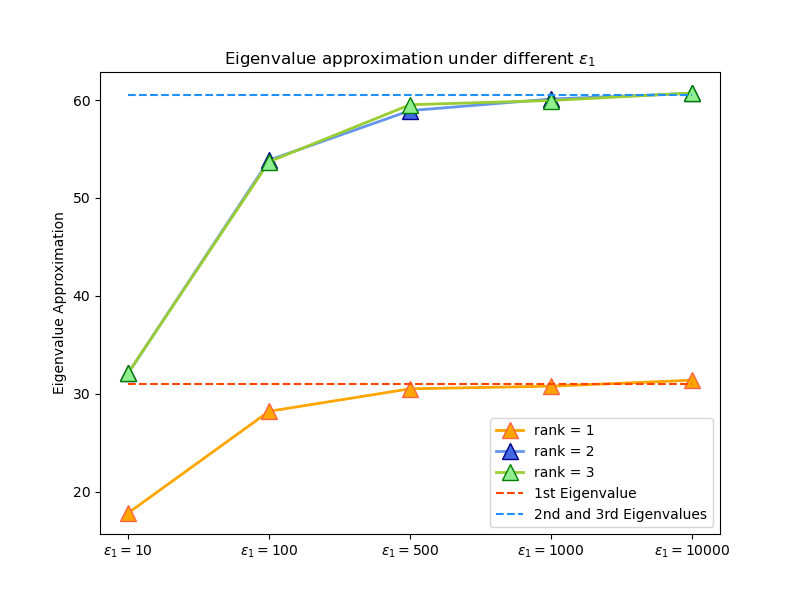
\includegraphics[width=0.7\textwidth]{figures1/EigFig2023/under-different-lambda1.png}
%     \caption{Eigenvalue approximation under different $\varepsilon_1$}\label{lambda1}
%     \label{fig:lambda1}
% \end{figure}

% 首先，我们选取不同的 $\varepsilon_1$ 值并使用 Deep Ritz 方法进行求解。所得结果展示于图 \ref{fig:lambda1}。定理 \ref{mainthm} 指出，随着 $\varepsilon_1$ 的增加，计算得到的特征值将趋近于真实值，实验结果验证了这一观察结论。

% 接下来，我们将讨论 $\varepsilon_2$ 对解的影响。我们选取了满足以下条件的 $\varepsilon_2$ 值：小于 $2\lambda_1$，略大于 $2\lambda_1$ 但小于 $2\lambda_2$ 和 $2\lambda_3$，略大于 $2\lambda_2$ 和 $2\lambda_3$，以及显著大于 $2\lambda_2$ 和 $2\lambda_3$。相关结果呈现于图 \ref{fig:lambda2}。

% 根据定理 \ref{mainthm}，当 $\varepsilon_2$ 大于 $2\lambda_k$ 时，第 $k$ 个特征值是可以被计算出来的。实验结果也验证了这一论述。当 $\varepsilon_2=10<2\lambda_1$ 时，算法无法计算出任何特征值。当 $2\lambda_1<\varepsilon_2=62<2\lambda_2$ 时，第一个特征值能够被较好地计算出来，但无法收敛至第二个特征值。当 $\varepsilon_2>2\lambda_2$ 时，所有对应的特征值均可被准确计算。

% \begin{figure}[htbp]
%     \centering
%     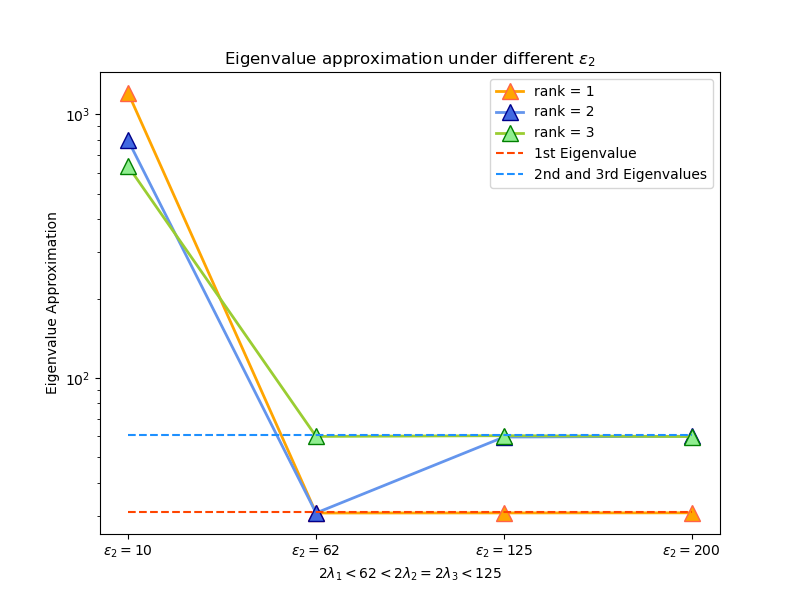
\includegraphics[width=0.6\textwidth]{figures1/EigFig2023/under-different-lambda2.png}
%     \caption{Eigenvalue approximation under different $\varepsilon_2$}
%     \label{fig:lambda2}
% \end{figure}

% 值得注意的是，当 $\varepsilon_2=62$ 时，第三个特征值似乎已被正确计算，这可能令人费解。为了阐明这一点，我们需要借助近似特征函数的热力图，如图 \ref{fig:heatmap} 所示。众所周知，在二维情形下，第二和第三个特征值在数值上相等，但对应于两个正交的特征函数。通过特征函数的热力图可以观察到，在计算第二个特征值时，由于 $\varepsilon_2$ 取值较小，解退化为了第一个特征函数。然而，在计算第三个特征值时，损失函数包含了两个与第一个特征值相关的正交项。因此，这等价于使用 $2\varepsilon_2$ 计算第二个特征值。这一观察结果与我们的理论分析保持一致。
% \begin{figure}[htbp]
%     \centering
%     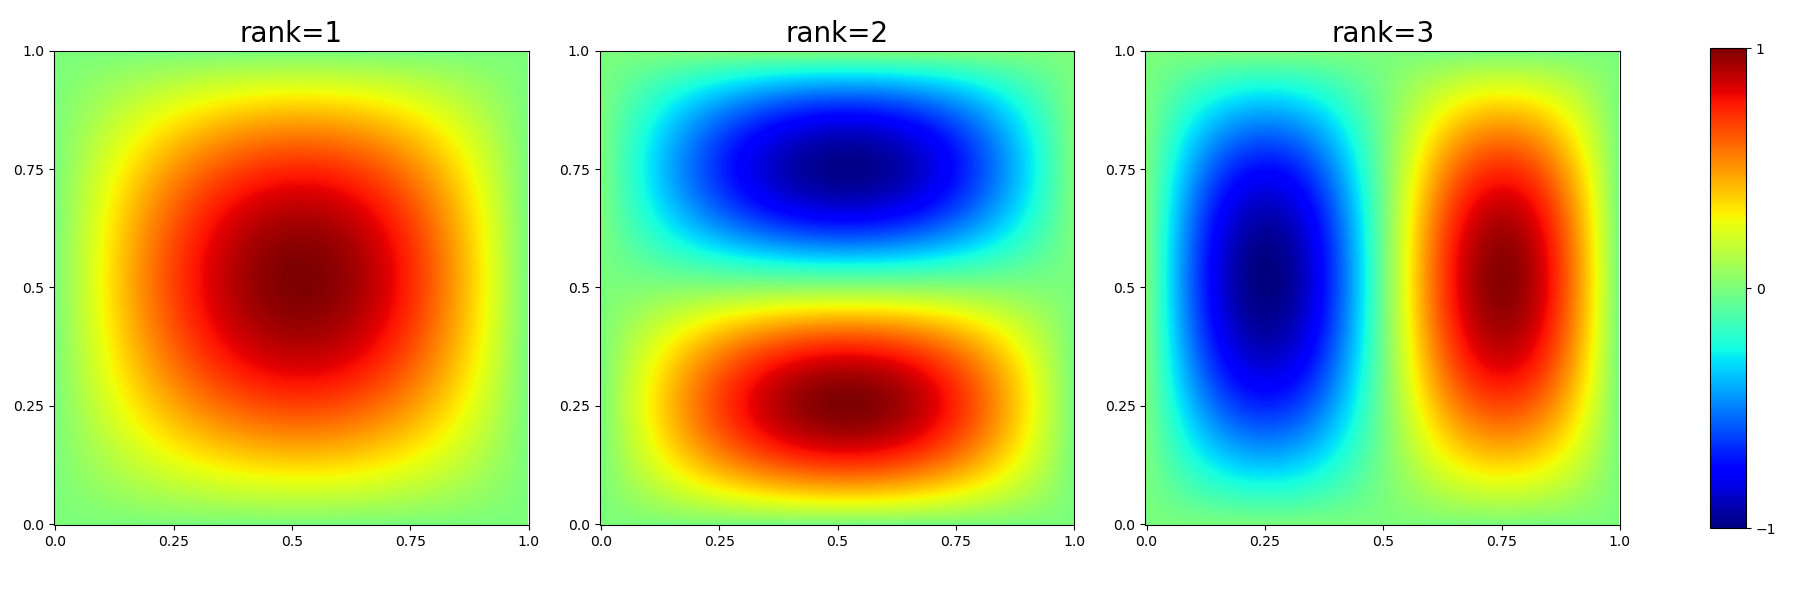
\includegraphics[width=0.8\textwidth]{figures1/EigFig2023/heat-map-reference.png}
%     \caption{Eigenfunction reference}
% \end{figure}
% \begin{figure}[htbp]
%     \centering
%     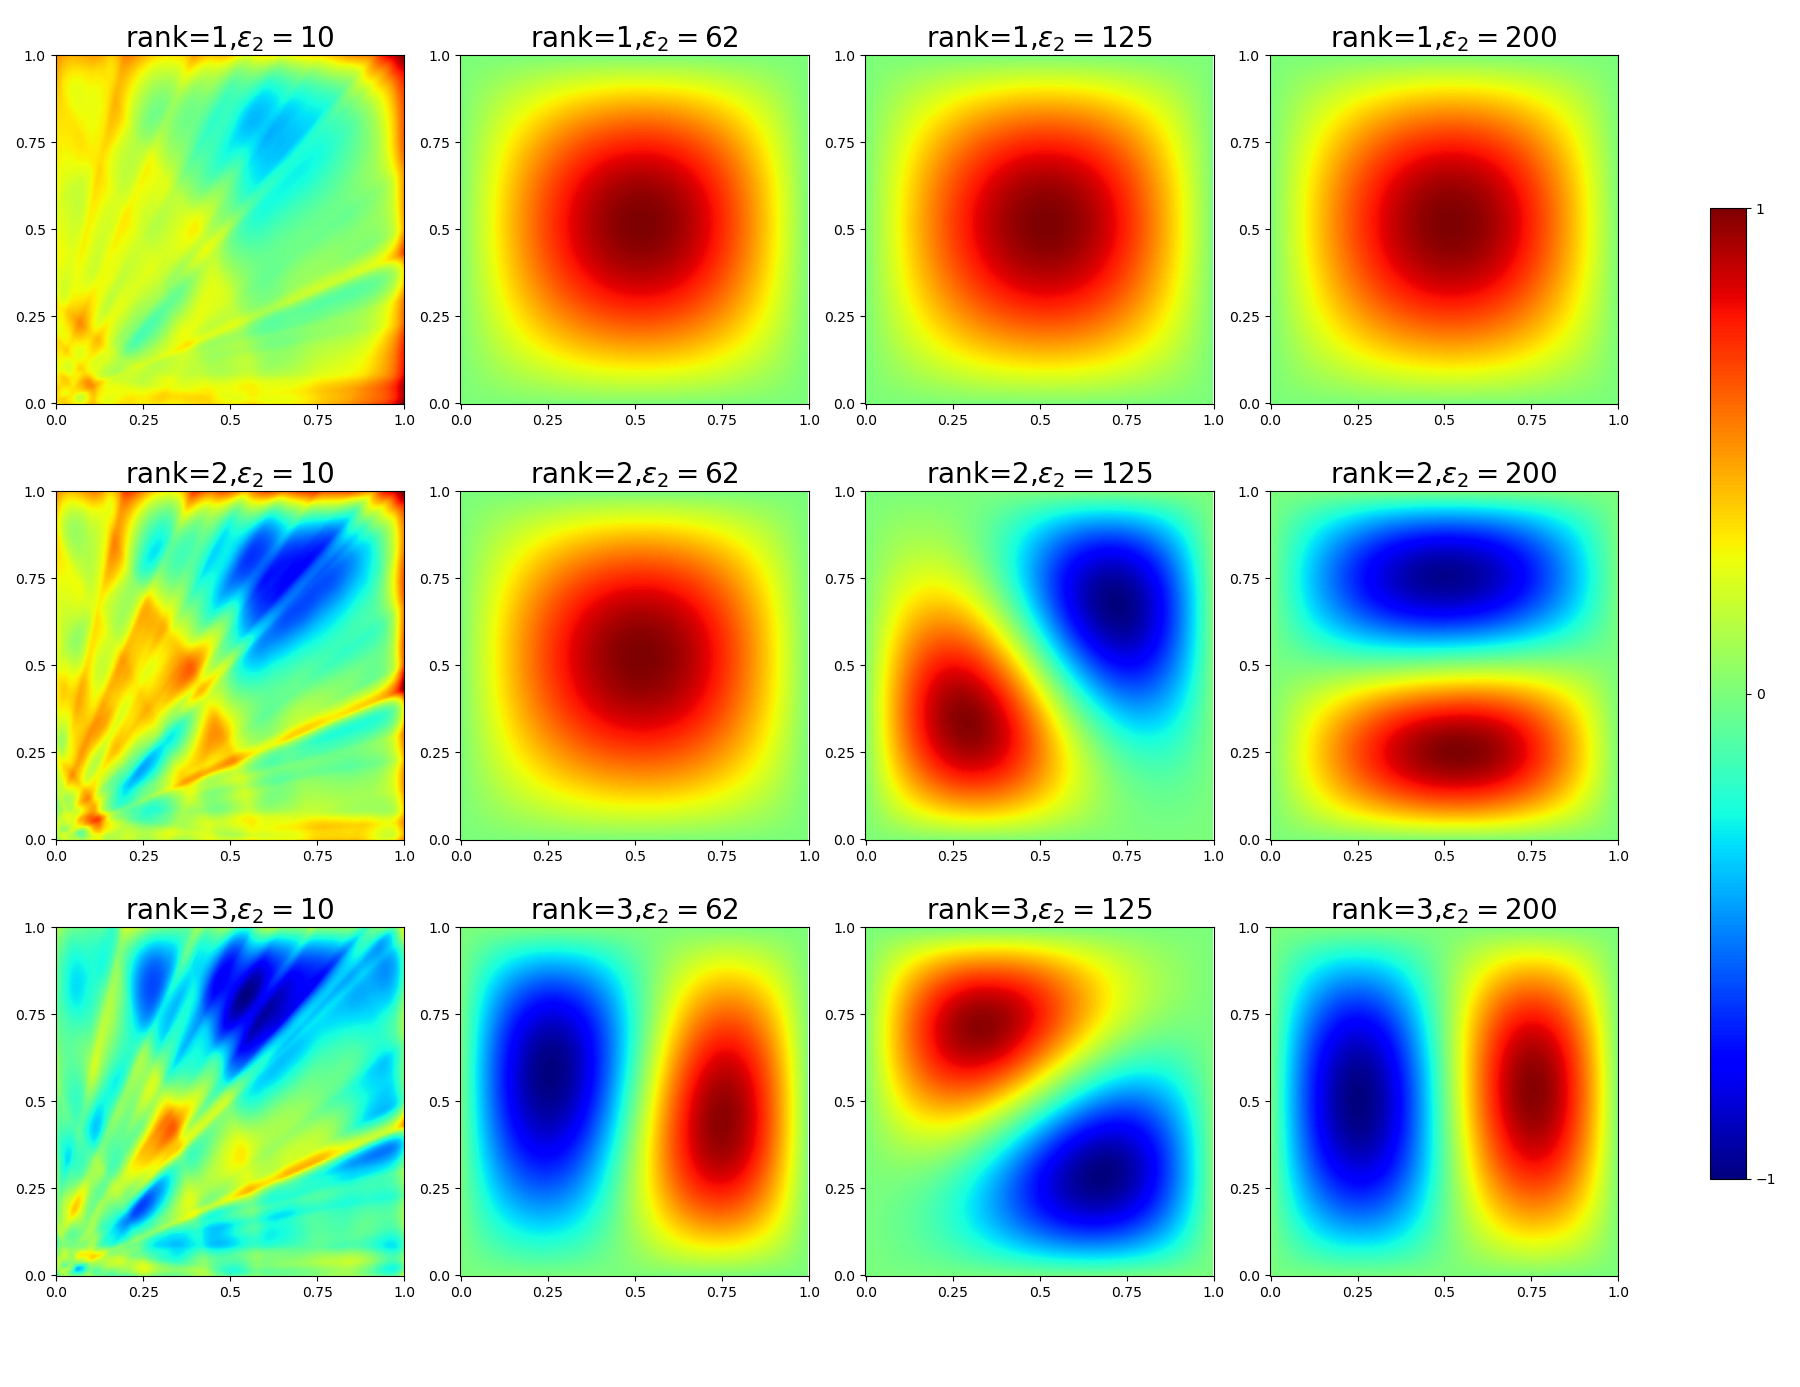
\includegraphics[width=0.8\textwidth]{figures1/EigFig2023/heat-map.png}
%     \caption{Heatmap for eigenfunction approximation for $\varepsilon_2=125$ and $\varepsilon_2=200$. }\label{fig:heatmap}
% \end{figure}

% 最后，我们考察了网络宽度和采样大小对解的影响。正如预期的那样，通过增加网络宽度和扩大采样规模，我们通常能够获得更精确的解

% \begin{figure}[htbp]
%     \centering
%     % 第一个子图
%     \begin{subfigure}{0.45\textwidth}
%         \centering
%         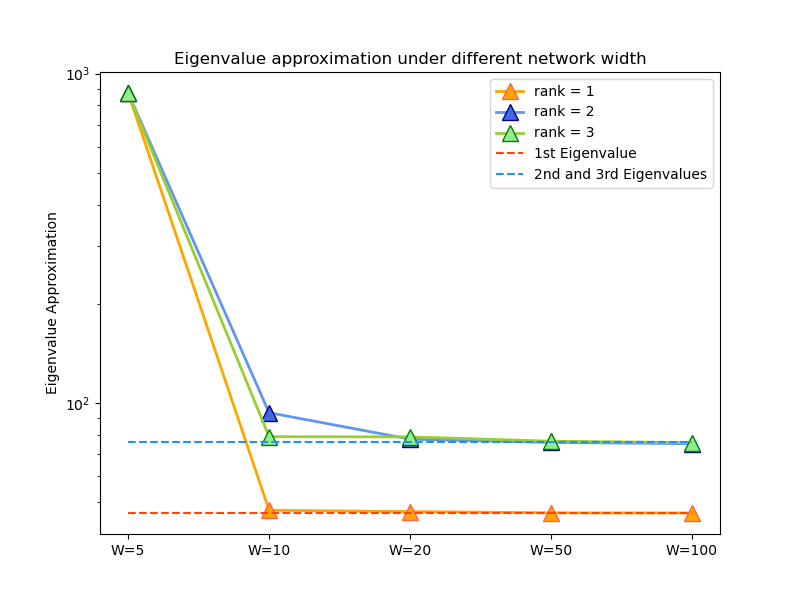
\includegraphics[width=\linewidth]{figures1/EigFig2023/under-different-width.png}
%         \caption{不同 $\mathcal{W}$ 下的特征值逼近}
%         \label{fig:width}
%     \end{subfigure}
%     \hfill % 关键：把两图撑开到两边
%     % 第二个子图
%     \begin{subfigure}{0.45\textwidth}
%         \centering
%         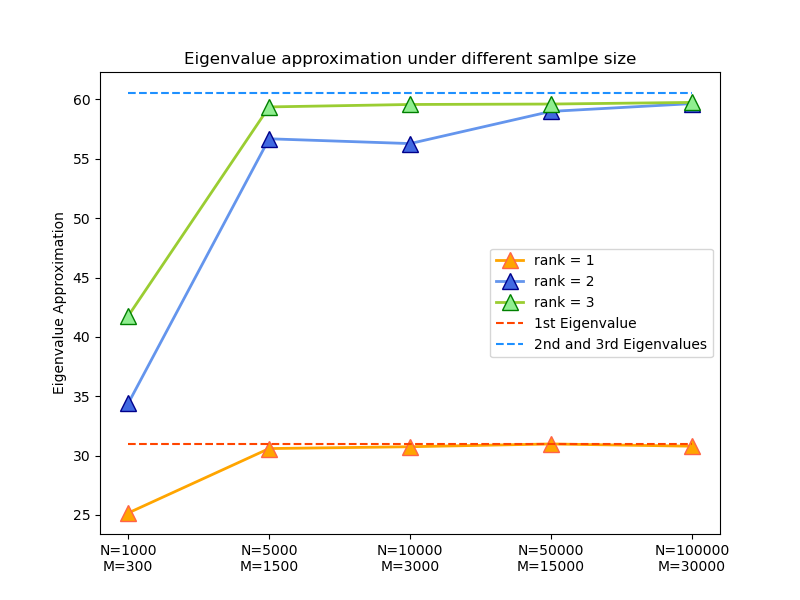
\includegraphics[width=\linewidth]{figures1/EigFig2023/under-different-sample.png}
%         \caption{不同样本量下的特征值逼近}
%         \label{fig:sample}
%     \end{subfigure}
    
%     \caption{网络宽度和采样大小的影响}
%     \label{fig:main}
% \end{figure}

% \subsection{立方体区域上的拉普拉斯特征值问题}\label{sec:10dcube}
% 在本节及下一节中，我们在 Eq.~\eqref{eq:conloss} 中选取了不同的函数 $w(x)$，包括常用的函数，如指数函数 $(w(x)=\exp(-\pi x))$ 和平方函数 $(w(x)=x^2)$。此外，我们探索了不同的区域，包括 10 维立方体和 10 维球体。在这些区域上，依赖于空间离散化的传统数值算法（如有限元法和有限差分法）一直无法提供令人满意的结果。实验的参数设置如下：

% \begin{table}[htbp]
% \centering
% \begin{tabular}{l|ccc}
% \toprule
% {\heiti 参数} & {\heiti 平方势} & \multicolumn{1}{p{2.2cm}}{{\heiti 指数势}} & \multicolumn{1}{p{3.2cm}}{{\heiti 简谐振子}}\\
% \midrule
% 区域 & $[0,1]^{10}$ &  $[0,1]^{10}$ & $\mathbb{R}^{10}$ 中的单位球 \\
% 学习率 & 0.001& 0.001& 0.001\\
% 训练轮数 (Epoch)& 100000& 100000& 50000\\
% $\varepsilon_1/\varepsilon_2$& 2000/1000&  2000/500& 2000/600\\
% 宽度/深度
% & 150/4 & 150/4 & 60/4 \\
% 样本量 ($\Omega$)& 200000& 200000& 200000\\
% 样本量 ($\partial\Omega$)& 80000& 80000& 80000\\
% \bottomrule
% \end{tabular}
% \caption{第 \ref{sec:10dcube} 节和第 \ref{sec:10dball} 节中的参数设置。}
% \end{table}

% \begin{figure}[htbp]
%     \centering
    
%     % --- 第一行 ---
%     % 创建一个子图容器，宽度约为页面宽度的一半
%     \begin{subfigure}{0.48\linewidth}
%         \centering
%         % 图片宽度占满当前子图容器
%         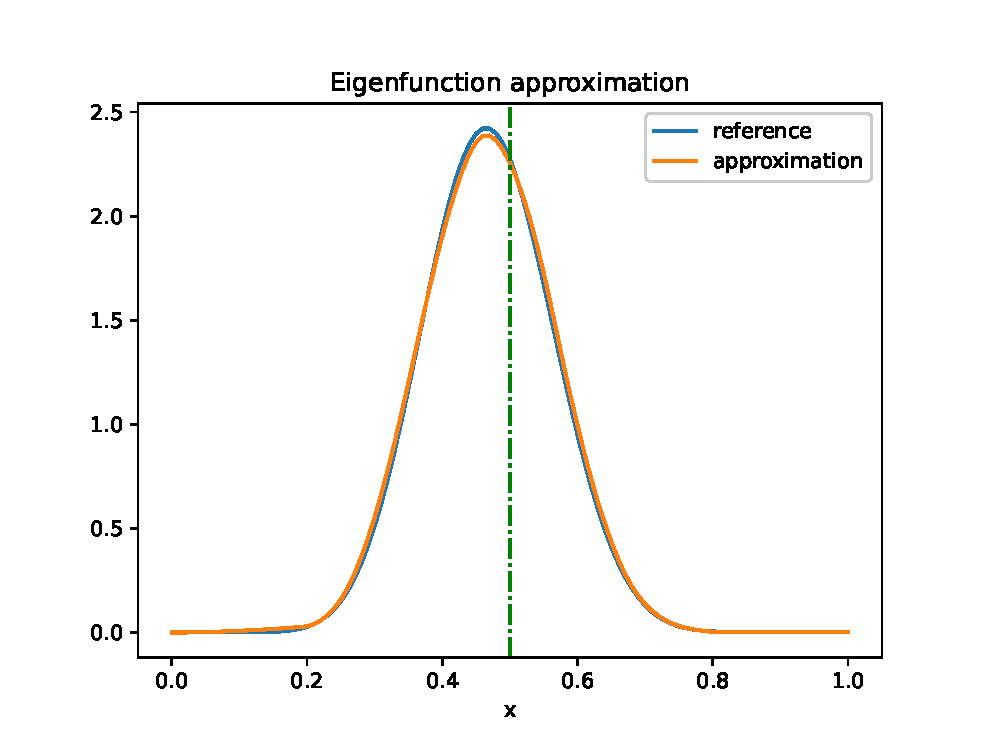
\includegraphics[width=\linewidth]{figures1/1square/unn_rank1.eps}
%         \caption{方形势下的 $\widehat{\xi}_{\phi 1}$}
%         \label{fig:sq1}
%     \end{subfigure}
%     \hfill % 弹性填充，将两个子图推向两侧
%     \begin{subfigure}{0.48\linewidth}
%         \centering
%         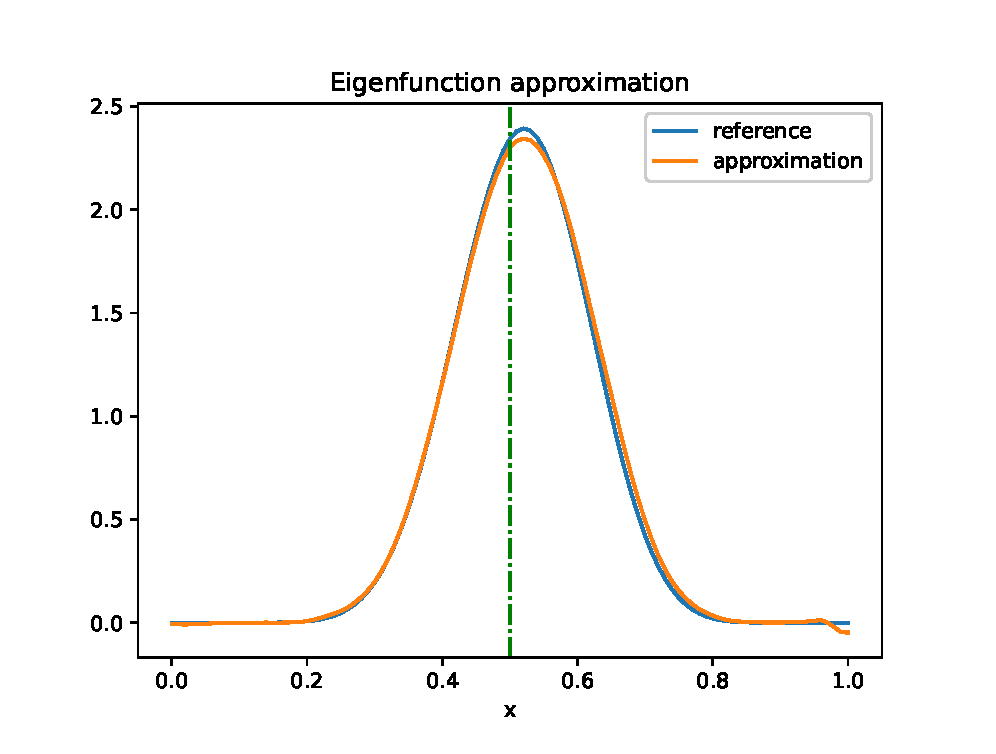
\includegraphics[width=\linewidth]{figures1/1expc/unn_rank1.eps}
%         \caption{指数势下的 $\widehat{\xi}_{\phi 1}$}
%         \label{fig:exp1}
%     \end{subfigure}
    
%     \vspace{1em} % 增加行间距
    
%     % --- 第二行 ---
%     \begin{subfigure}{0.48\linewidth}
%         \centering
%         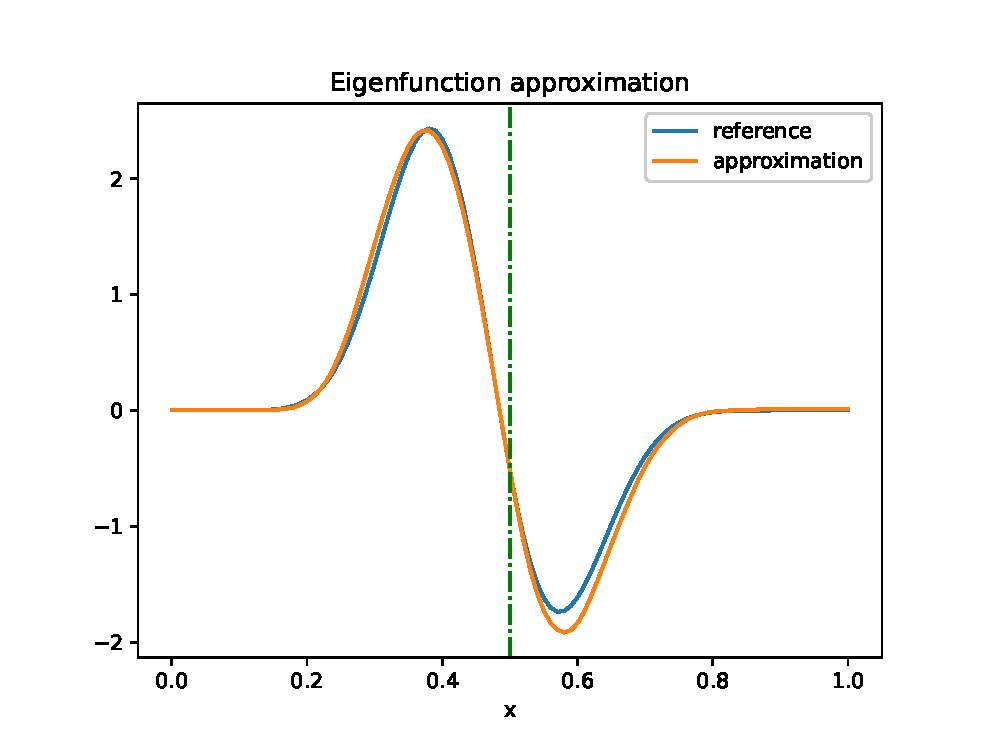
\includegraphics[width=\linewidth]{figures1/2square/unn_rank2.eps}
%         \caption{方形势下的 $\widehat{\xi}_{\phi 2}$}
%         \label{fig:sq2}
%     \end{subfigure}
%     \hfill
%     \begin{subfigure}{0.48\linewidth}
%         \centering
%         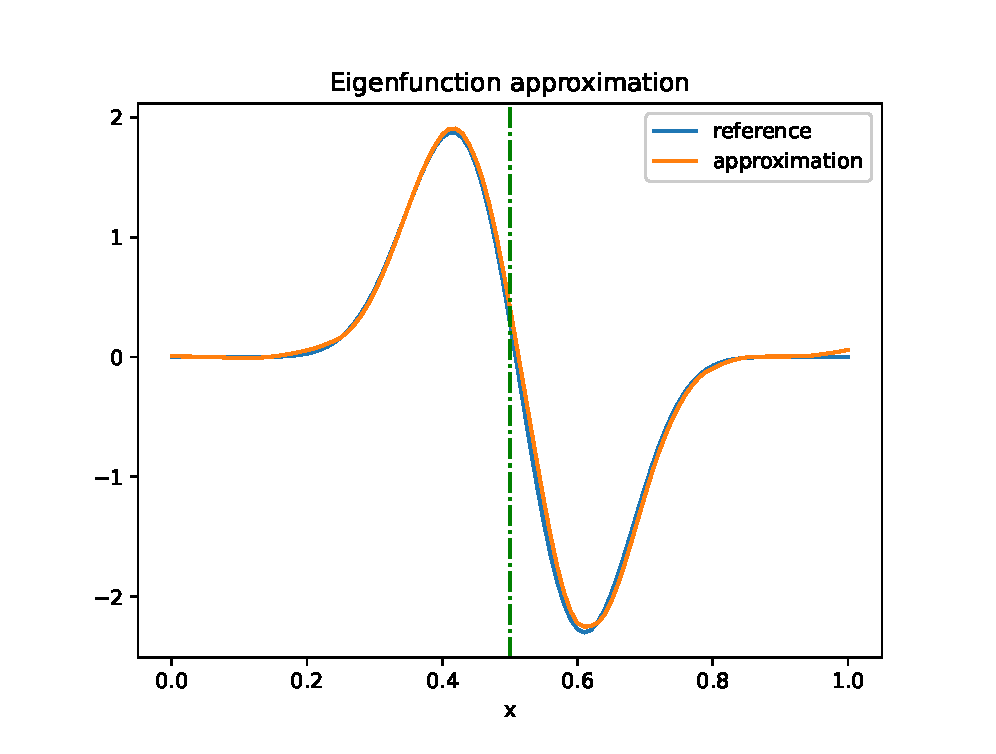
\includegraphics[width=\linewidth]{figures1/2expc/unn_rank2.eps}
%         \caption{指数势下的 $\widehat{\xi}_{\phi 2}$}
%         \label{fig:exp2}
%     \end{subfigure}
    
%     \vspace{1em} % 增加行间距
    
%     % --- 第三行 ---
%     \begin{subfigure}{0.48\linewidth}
%         \centering
%         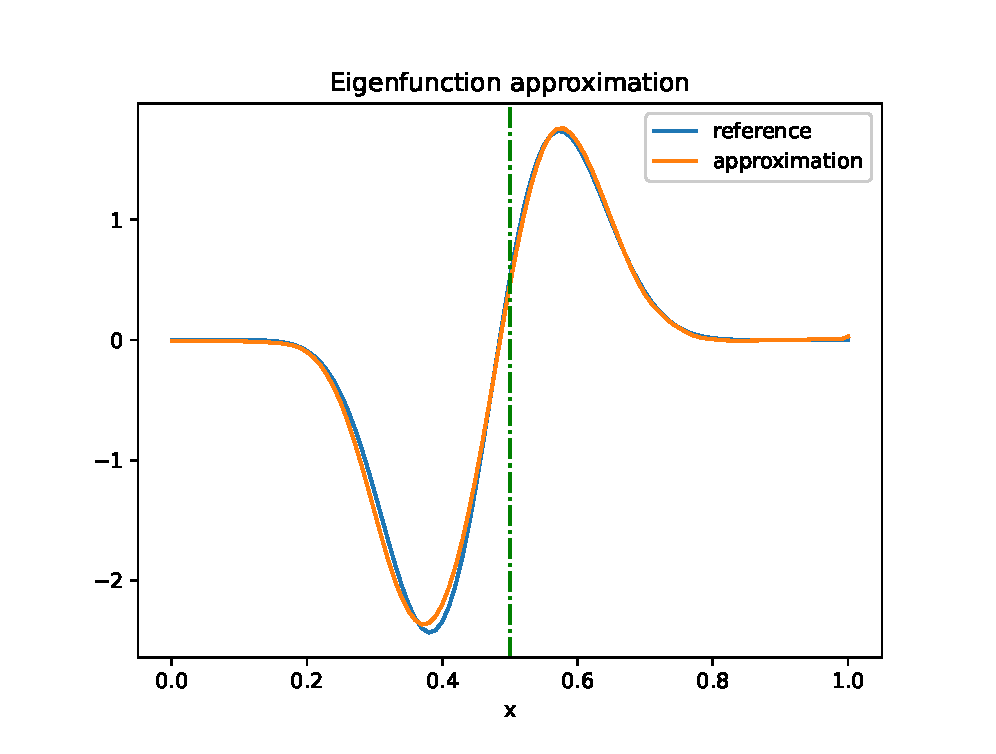
\includegraphics[width=\linewidth]{figures1/3square/unn_rank3.eps}
%         \caption{方形势下的 $\widehat{\xi}_{\phi 3}$}
%         \label{fig:sq3}
%     \end{subfigure}
%     \hfill
%     \begin{subfigure}{0.48\linewidth}
%         \centering
%         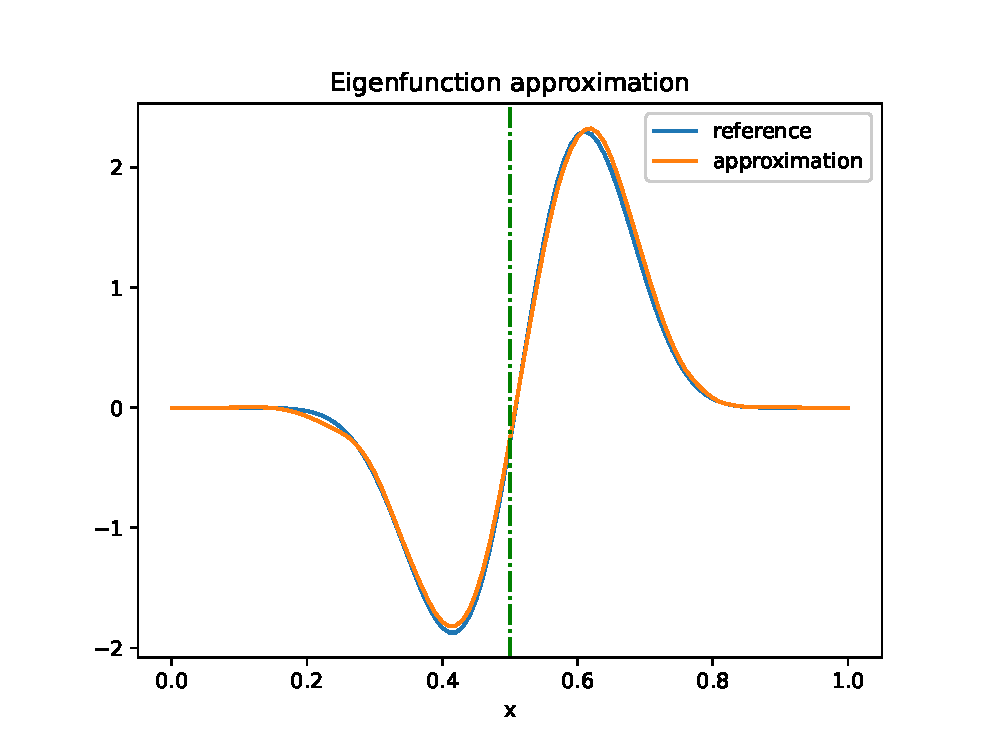
\includegraphics[width=\linewidth]{figures1/3expc/unn_rank3.eps}
%         \caption{指数势下的 $\widehat{\xi}_{\phi 3}$}
%         \label{fig:exp3}
%     \end{subfigure}
    
%     % 总标题
%     \caption{方形势和指数势在立方体区域对角线上的本征函数。}
%     \label{fig1}
% \end{figure}

% \begin{figure}[htbp]
%     \centering
    
%     % --- 第一行：lambda_1 ---
%     \begin{subfigure}{0.48\textwidth}
%         \centering
%         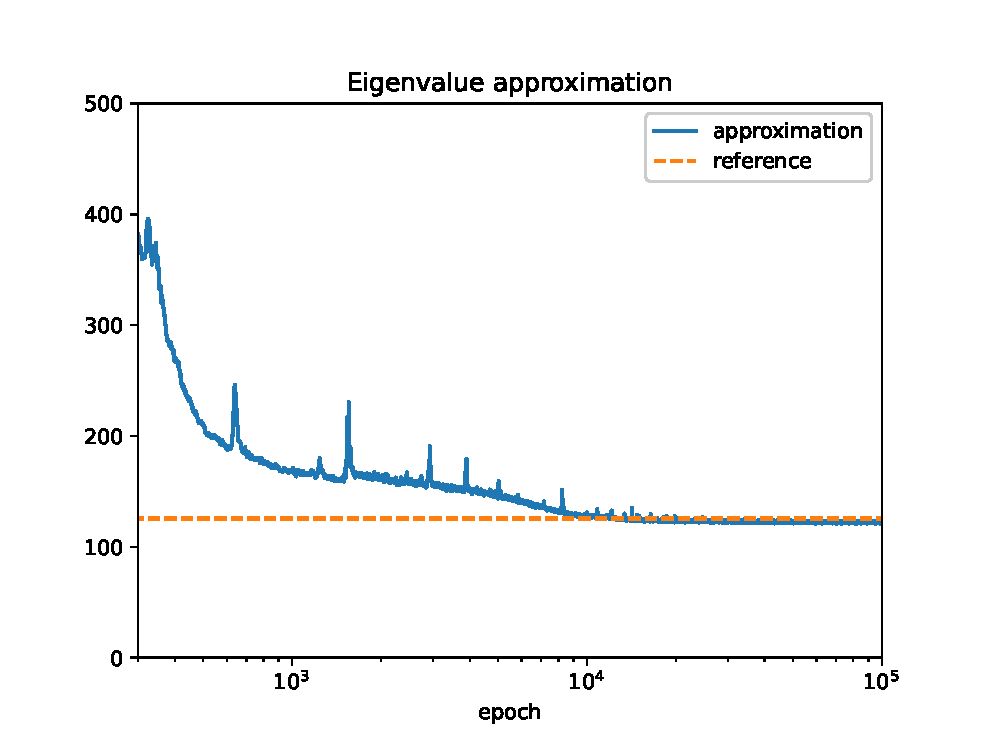
\includegraphics[width=\linewidth]{figures1/1square/eigenvalue_rank1.eps}
%         \caption{方势的 $\lambda_{1}$}
%     \end{subfigure}
%     \hfill
%     \begin{subfigure}{0.48\textwidth}
%         \centering
%         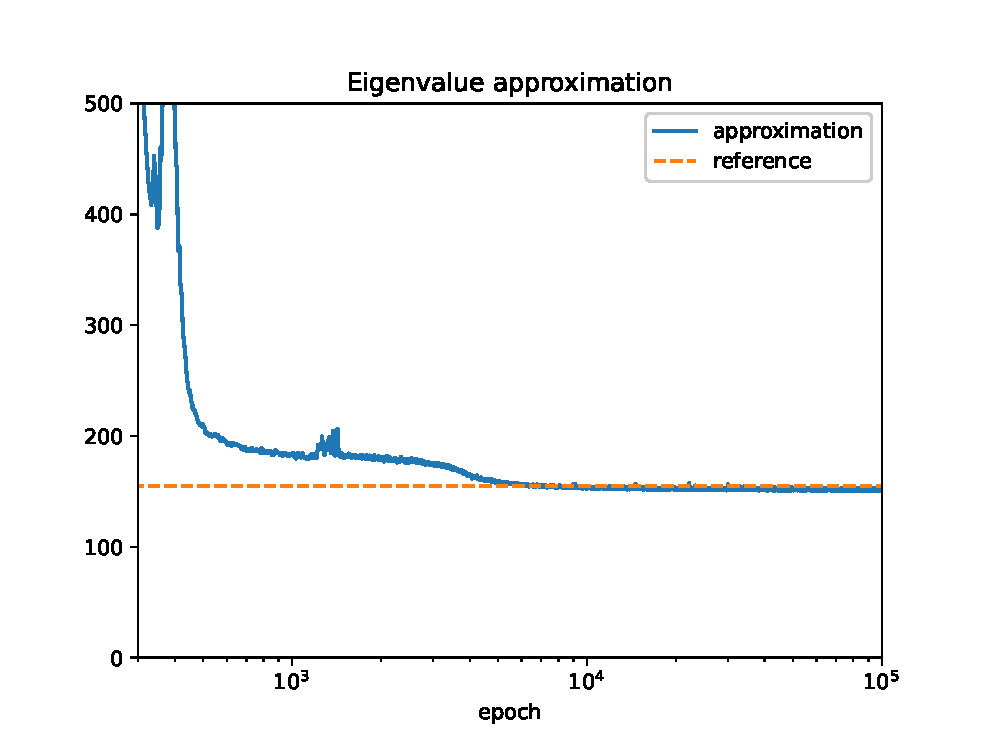
\includegraphics[width=\linewidth]{figures1/1expc/eigenvalue_rank1.eps}
%         \caption{指数势的 $\lambda_{1}$}
%     \end{subfigure}
    
%     \vspace{1em} % 增加行间距
    
%     % --- 第二行：lambda_2 ---
%     \begin{subfigure}{0.48\textwidth}
%         \centering
%         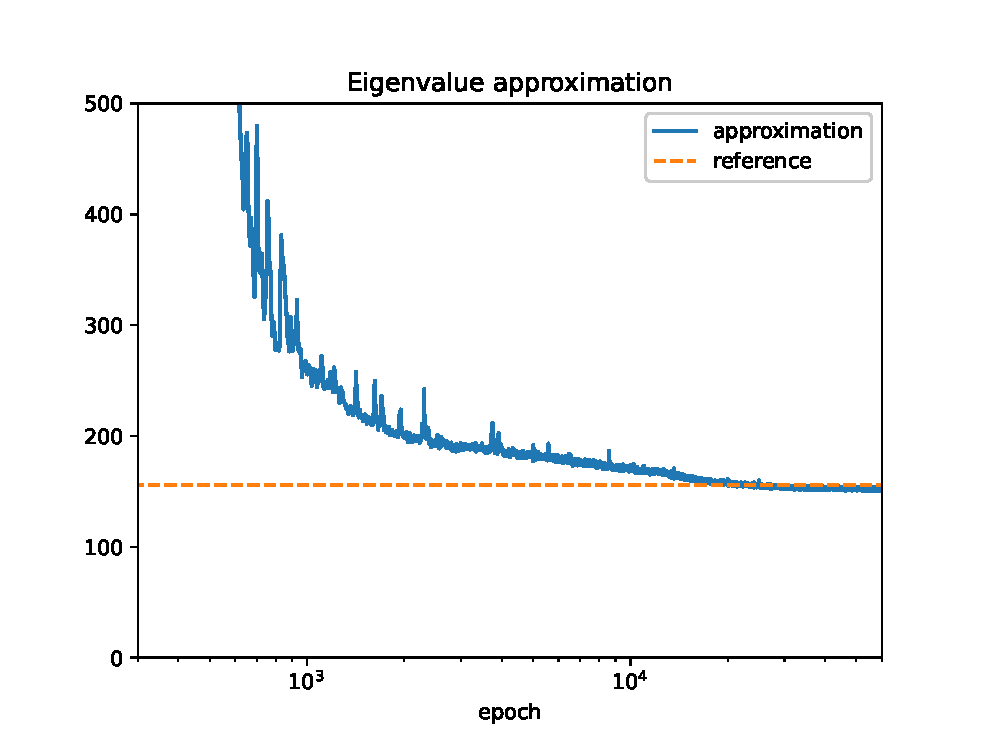
\includegraphics[width=\linewidth]{figures1/2square/eigenvalue_rank2.eps}
%         \caption{方势的 $\lambda_{2}$}
%     \end{subfigure}
%     \hfill
%     \begin{subfigure}{0.48\textwidth}
%         \centering
%         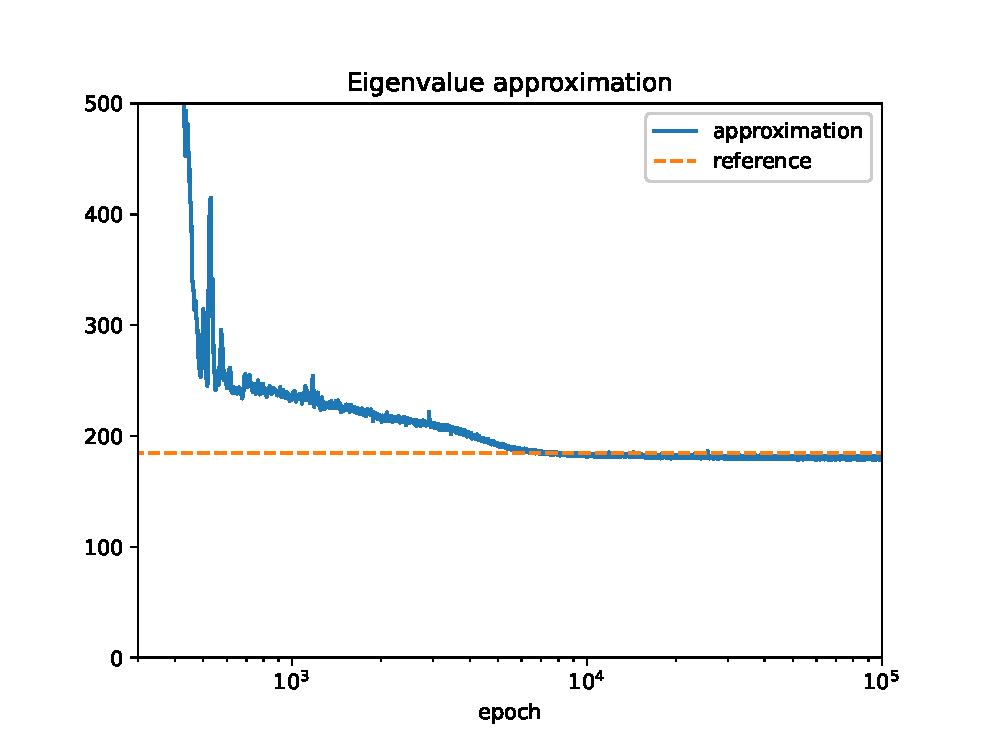
\includegraphics[width=\linewidth]{figures1/2expc/eigenvalue_rank2.eps}
%         \caption{指数势的 $\lambda_{2}$}
%     \end{subfigure}
    
%     \vspace{1em} % 增加行间距
    
%     % --- 第三行：lambda_3 ---
%     \begin{subfigure}{0.48\textwidth}
%         \centering
%         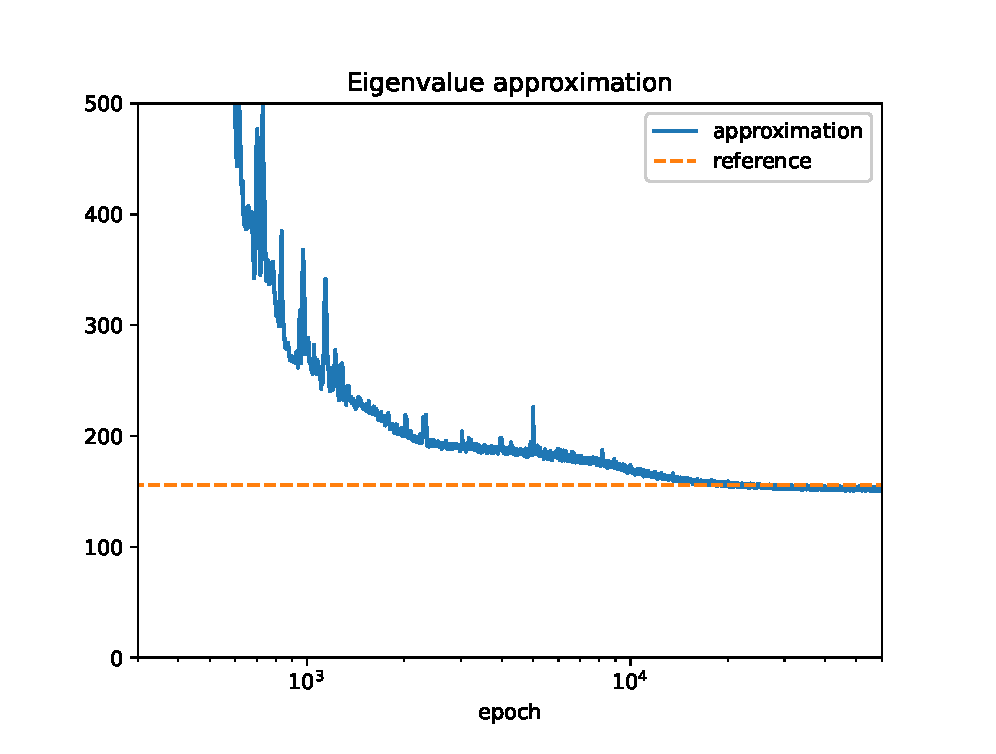
\includegraphics[width=\linewidth]{figures1/3square/eigenvalue_rank3.eps}
%         \caption{方势的 $\lambda_{3}$}
%     \end{subfigure}
%     \hfill
%     \begin{subfigure}{0.48\textwidth}
%         \centering
%         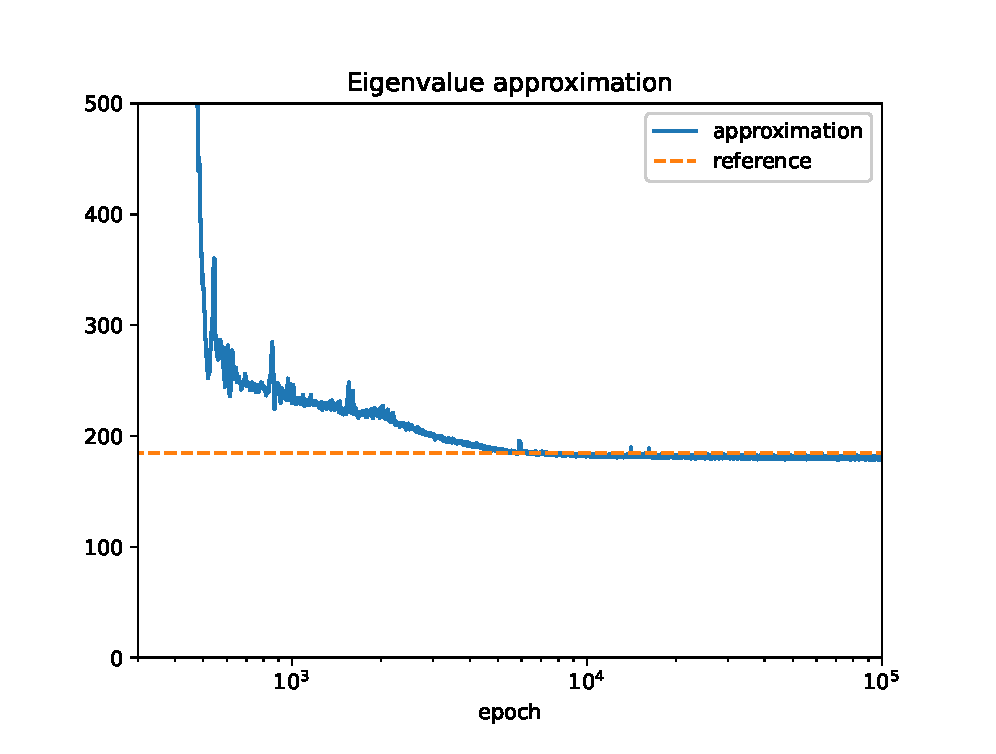
\includegraphics[width=\linewidth]{figures1/3expc/eigenvalue_rank3.eps}
%         \caption{指数势的 $\lambda_{3}$}
%     \end{subfigure}
    
%     % 总标题
%     % 这一段红字依赖 \usepackage{xcolor}
%     \caption{训练过程中方势与指数势的特征值逼近情况。}
%     \label{fig2}
% \end{figure}

% 如图 \ref{fig1} 和 \ref{fig2} 所示，所有估计的特征值和特征函数均与其各自的精确值非常接近。计算得到的特征值小于精确值，这与定理 \ref{mainthm} 的结论相符。

% \subsection{单位球上的拉普拉斯特征值问题}\label{sec:10dball}
% 在本节中，我们求解 $\mathbb{R}^{10}$ 和 $\mathbb{R}^{20}$ 空间中单位球的特征值问题。与上述情形不同，在此情形下，由于受到无限深势阱的束缚，所有的 $x_{i}$ 不再是独立运动的：
% \begin{equation*}
% V(x)=\left\{
% \begin{array}{ll}
% 0&|x|<1,\\
% +\infty&|x|\geq 1.
% \end{array}\right.
% \end{equation*}
% 在此情形下，第一特征值 $\lambda_{1}$ 是四阶贝塞尔函数的第一根，而第二特征值 $\lambda_{2}$ 是五阶贝塞尔函数的第一根。所有对应的特征函数可表示为：
% \begin{equation*}
% \xi_{k}(x)\in\mathop{span}\left\{ \frac{1}{\left(\lambda_{k}|x|\right)^{4+l}}J_{4+l}(\lambda_{k}|x|)P_{l}(x),\quad l=0,1,2,\cdots, \quad k=1,2,3,\cdots .\right\},
% \end{equation*}
% 其中 $P_{l}(x)$ 是一个 $l$ 次齐次多项式。

% \begin{figure}[htbp]
%     \centering
    
%     % --- 第一行 (Rank 1) ---
%     \begin{subfigure}{0.48\textwidth}
%         \centering
%         % 使用 \linewidth 让图片自动适应子图容器的宽度
%         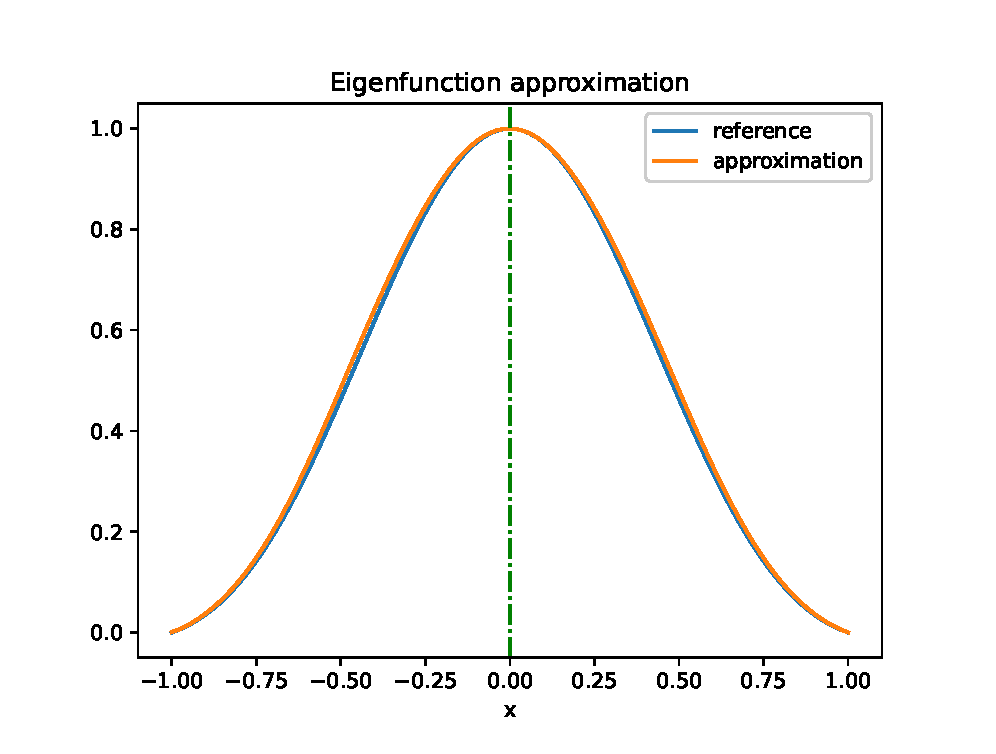
\includegraphics[width=\linewidth]{figures1/ball/ball_unn_rank1.eps}
%         \caption{单位球上的 $\widehat{\xi}_{\phi 1}$}
%     \end{subfigure}
%     \hfill % 左右推开
%     \begin{subfigure}{0.48\textwidth}
%         \centering
%         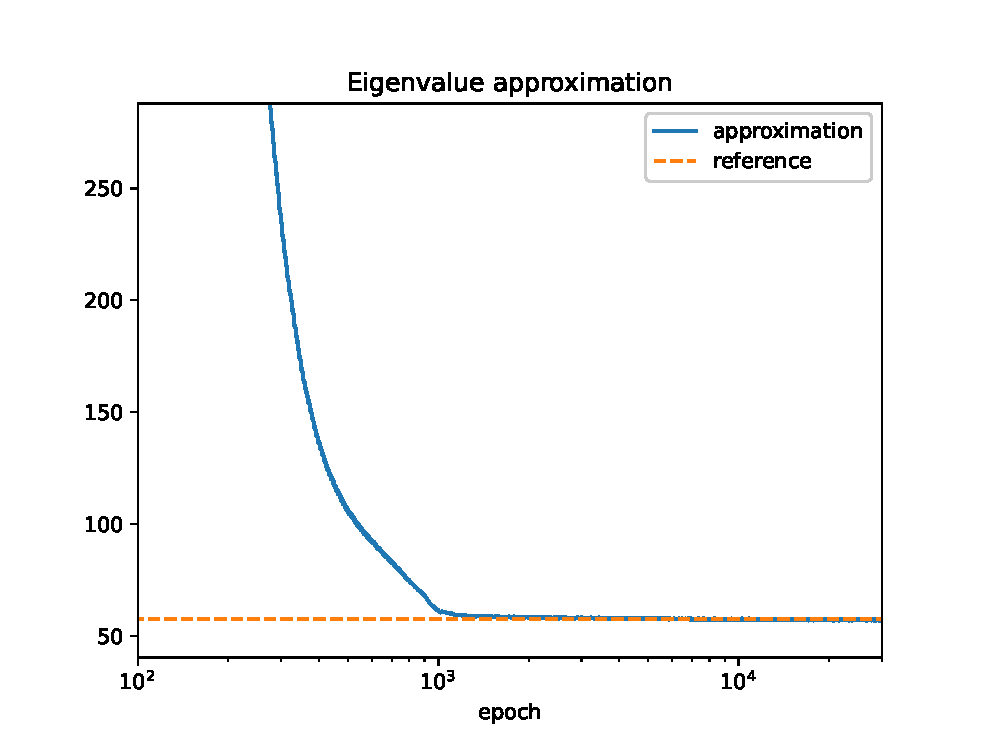
\includegraphics[width=\linewidth]{figures1/ball/ball_eigenvalue_rank1.eps}
%         \caption{单位球上的 $\lambda_{1}$}
%     \end{subfigure}
    
%     \vspace{0.5em} % 行间距，防止上下两行太挤
    
%     % --- 第二行 (Rank 2) ---
%     \begin{subfigure}{0.48\textwidth}
%         \centering
%         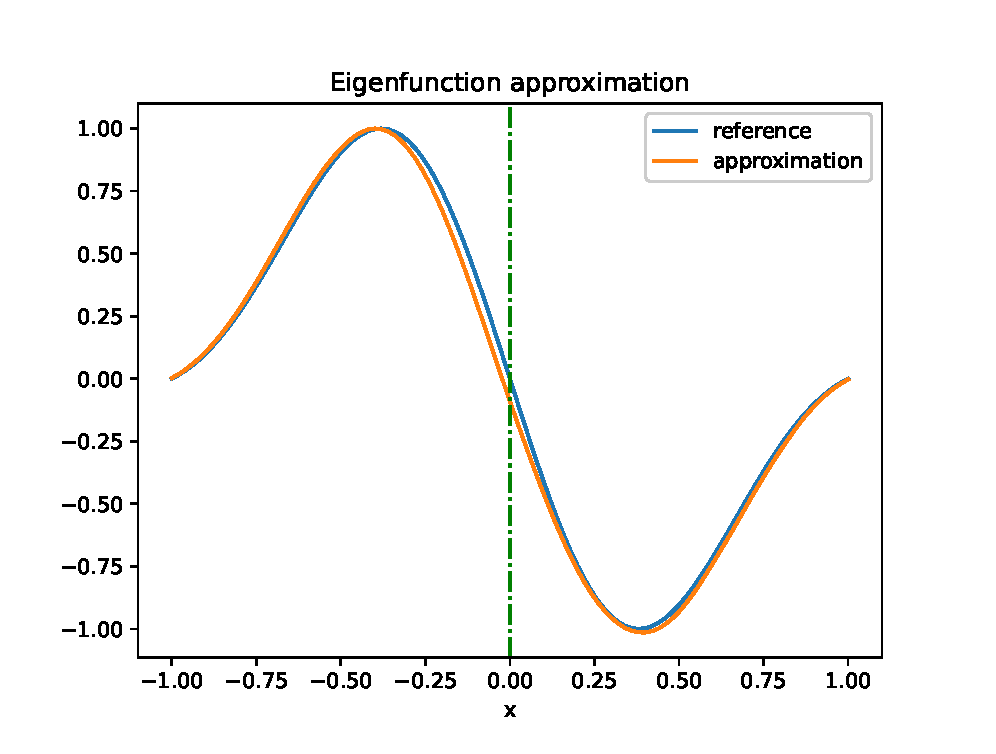
\includegraphics[width=\linewidth]{figures1/ball/ball_unn_rank2.eps}
%         \caption{单位球上的 $\widehat{\xi}_{\phi 2}$}
%     \end{subfigure}
%     \hfill
%     \begin{subfigure}{0.48\textwidth}
%         \centering
%         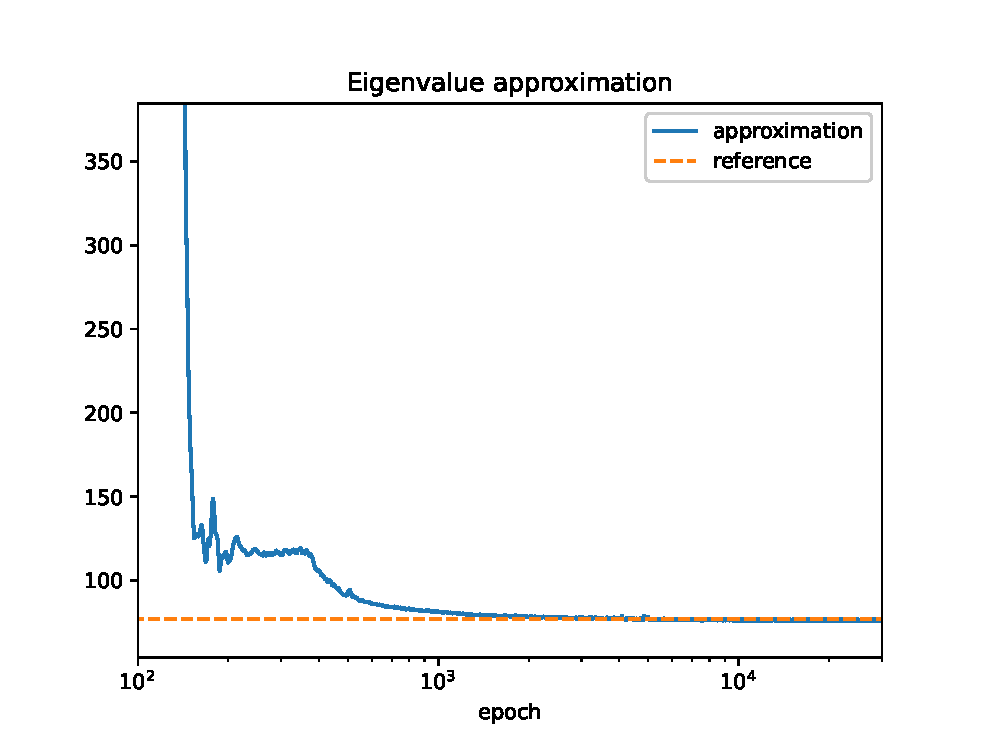
\includegraphics[width=\linewidth]{figures1/ball/ball_eigenvalue_rank2.eps}
%         \caption{单位球上的 $\lambda_{2}$}
%     \end{subfigure}
    
%     \vspace{0.5em} % 行间距
    
%     % --- 第三行 (Rank 3) ---
%     \begin{subfigure}{0.48\textwidth}
%         \centering
%         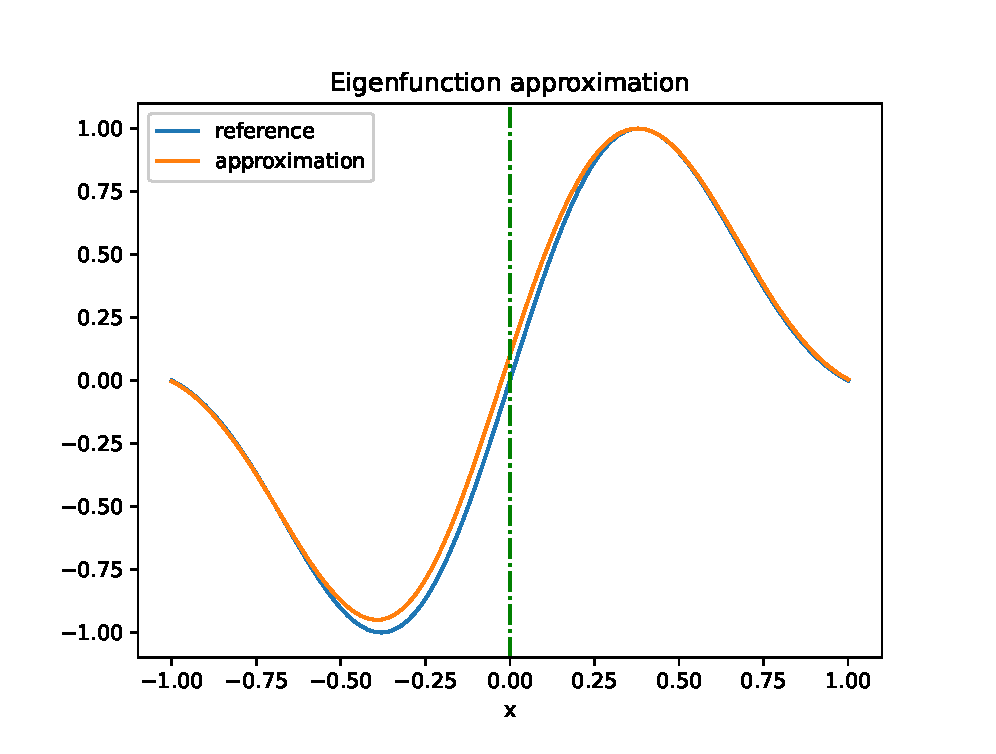
\includegraphics[width=\linewidth]{figures1/ball/ball_unn_rank3.eps}
%         \caption{单位球上的 $\widehat{\xi}_{\phi 3}$}
%     \end{subfigure}
%     \hfill
%     \begin{subfigure}{0.48\textwidth}
%         \centering
%         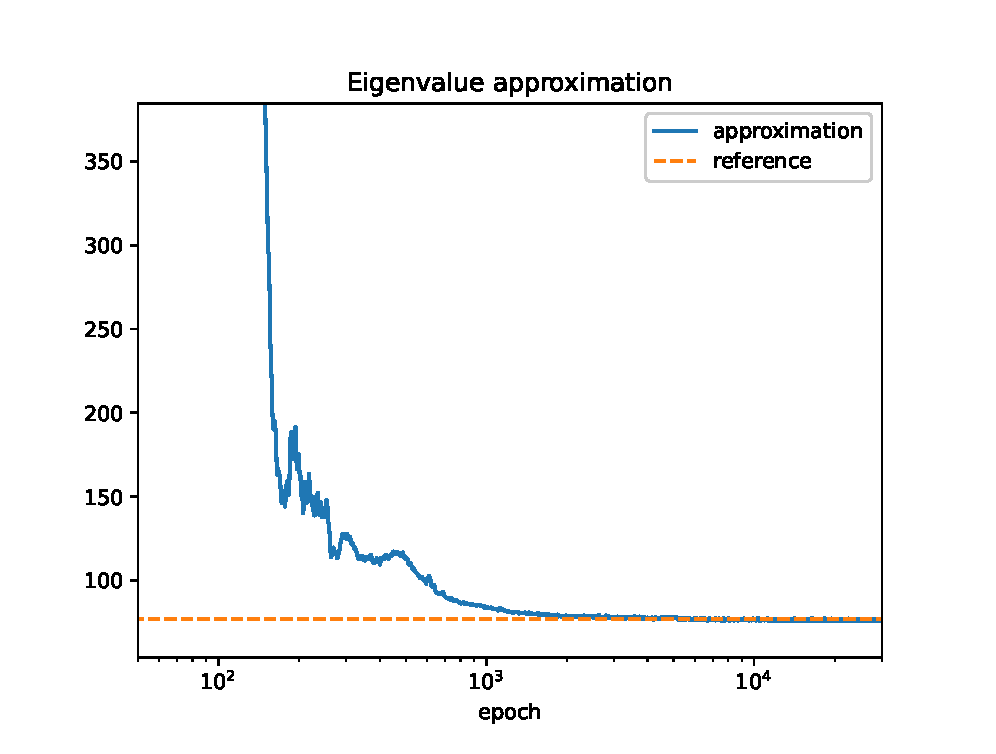
\includegraphics[width=\linewidth]{figures1/ball/ball_eigenvalue_rank3.eps}
%         \caption{单位球上的 $\lambda_{3}$}
%     \end{subfigure}
    
%     % --- 总标题 ---
%     \caption{左图：对应于 10 维单位球对角线上的特征函数。右图：随训练轮数（epoch）变化的对应特征值演化。}
%     \label{fig3}
% \end{figure}

% 对于 $\mathbb{R}^{10}$，结果展示在图 \ref{fig3} 中，在此设置下，所提出的方法很好地估计了特征值和特征函数。

% 对于 $\mathbb{R}^{20}$ 的情形，使用蒙特卡洛方法计算积分面临挑战。具体而言，高维空间区域中的均匀采样会导致采样点在边界附近过度集中。为了克服这一挑战，常见的策略包括增加采样点数量以及实施更高效的采样技术。作为一种解决方案，我们采用了分层采样方法。该方法将单位球划分为两个不同的区域，记为 $B_{20}(0,1/2)$ 和 $B_{20}(0,1)/B_{20}(0,1/2)$。我们对每个区域分别计算蒙特卡洛积分，随后将所得数值进行加权求和。

% 这种采样方法确保了采样在一定程度上能够捕捉到区域内部的信息，从而提升了算法的性能。实验结果展示在附图 \ref{fig:20dball} 中。

% \begin{table}[h]
% \centering
% \begin{tabular}{l|c}
% \toprule
% {\heiti 参数} & {\heiti 简谐振子}\\
% \midrule
% 区域 & $\mathbb{R}^{20}$ 中的单位球\\
% 学习率 & 0.001\\
% 第 1 个特征值的训练轮数 & 100000\\
% 第 2、3 个特征值的训练轮数 & 200000\\
% $\varepsilon_1/\varepsilon_2$ & 5000/3000\\
% 宽度/深度 & 120/4\\
% 样本数量 ($B_{20}(0,0.5)$) & 50000\\
% 样本数量 ($B_{20}(0,1)/B_{20}(0,0.5)$) & 500000\\
% 样本数量 ($\partial B_{20}(0,1)$) & 200000\\
% \bottomrule
% \end{tabular}
% \caption{参数设置}
% \end{table}

% \begin{figure}[htbp]
%     \centering
    
%     % --- 第一行：Rank 1 ---
%     \begin{subfigure}{0.48\textwidth}
%         \centering
%         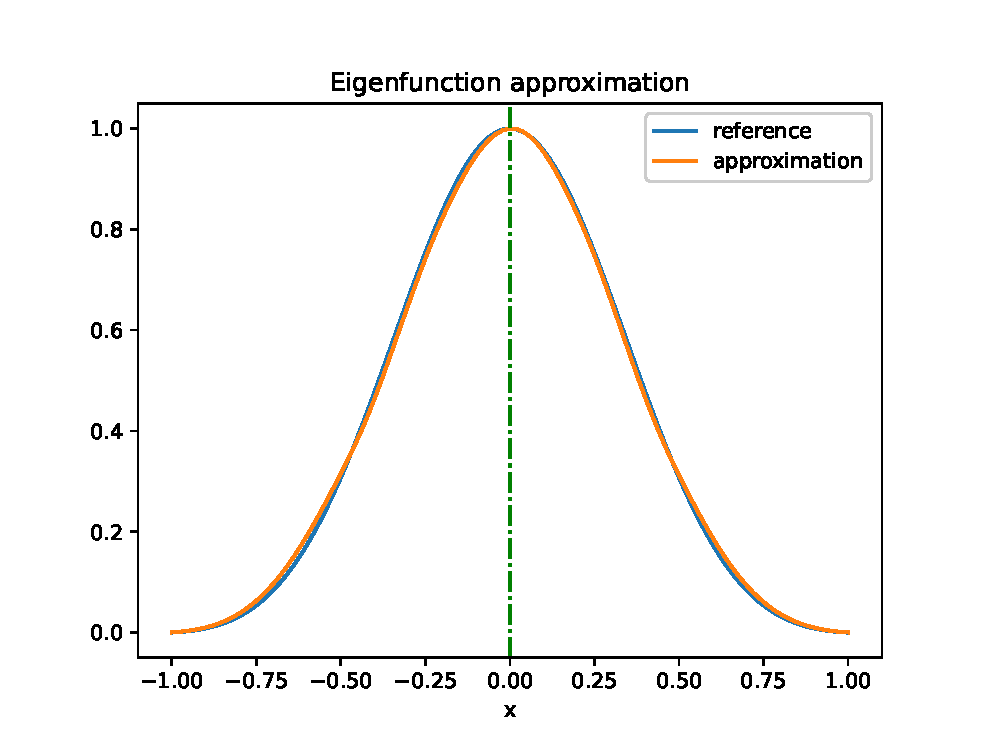
\includegraphics[width=\linewidth]{figures1/20d/unn_rank1.eps}
%         \caption{单位球上的 $\widehat{\xi}_{\phi 1}$}
%         \label{fig:xi_rank1}
%     \end{subfigure}
%     \hfill
%     \begin{subfigure}{0.48\textwidth}
%         \centering
%         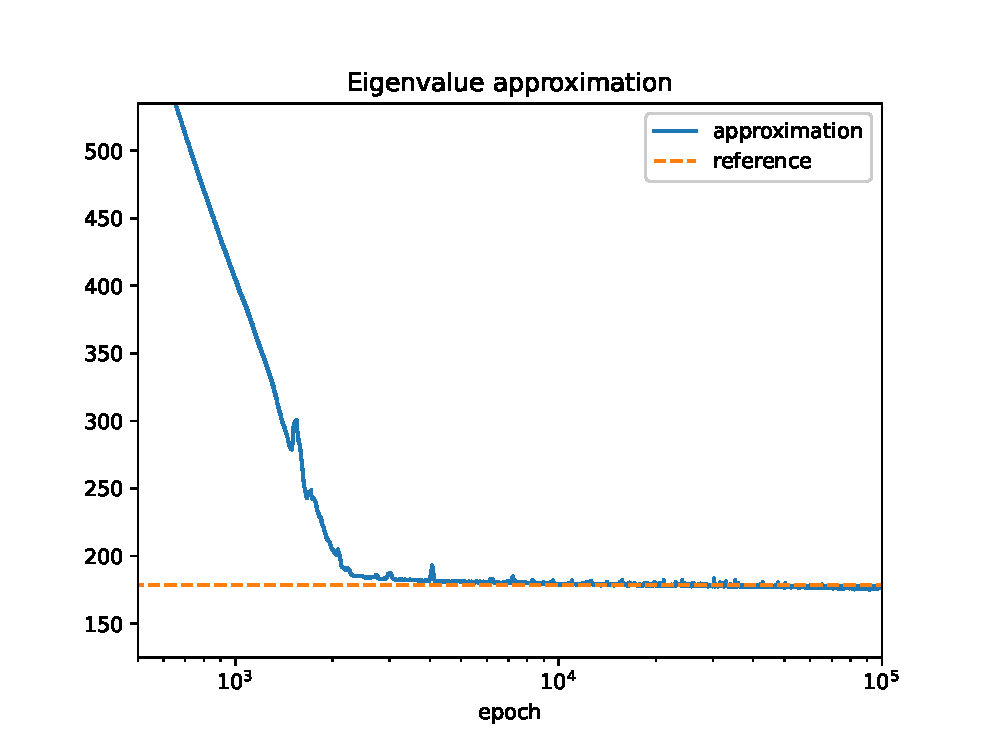
\includegraphics[width=\linewidth]{figures1/20d/eigenvalue_rank1.eps}
%         \caption{单位球上的 $\lambda_{1}$}
%         \label{fig:lambda_rank1}
%     \end{subfigure}
    
%     \vspace{1em} % 增加行间距
    
%     % --- 第二行：Rank 2 ---
%     \begin{subfigure}{0.48\textwidth}
%         \centering
%         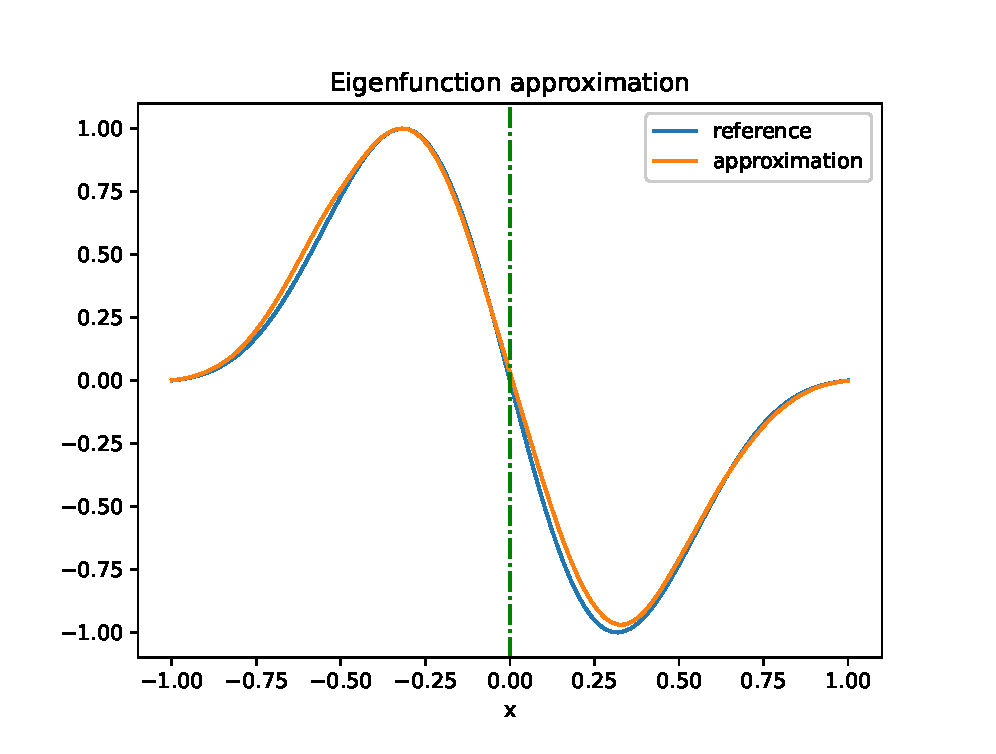
\includegraphics[width=\linewidth]{figures1/20d/unn_rank2.eps}
%         \caption{单位球上的 $\widehat{\xi}_{\phi 2}$}
%         \label{fig:xi_rank2}
%     \end{subfigure}
%     \hfill
%     \begin{subfigure}{0.48\textwidth}
%         \centering
%         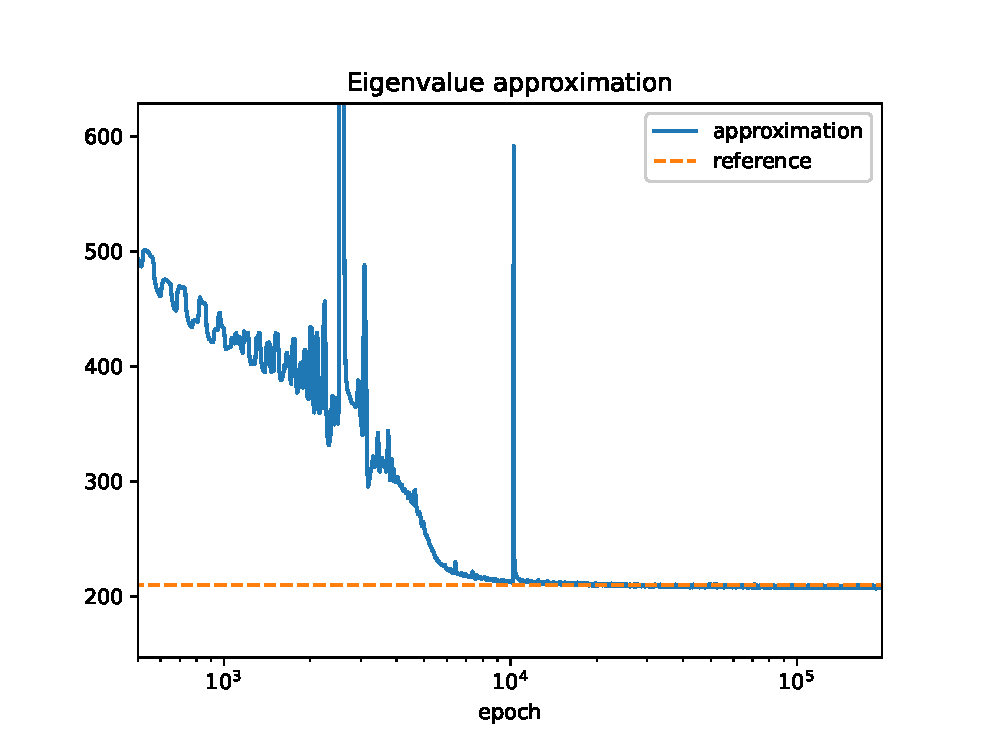
\includegraphics[width=\linewidth]{figures1/20d/eigenvalue_rank2.eps}
%         \caption{单位球上的 $\lambda_{2}$}
%         \label{fig:lambda_rank2}
%     \end{subfigure}
    
%     \vspace{1em} % 增加行间距
    
%     % --- 第三行：Rank 3 ---
%     \begin{subfigure}{0.48\textwidth}
%         \centering
%         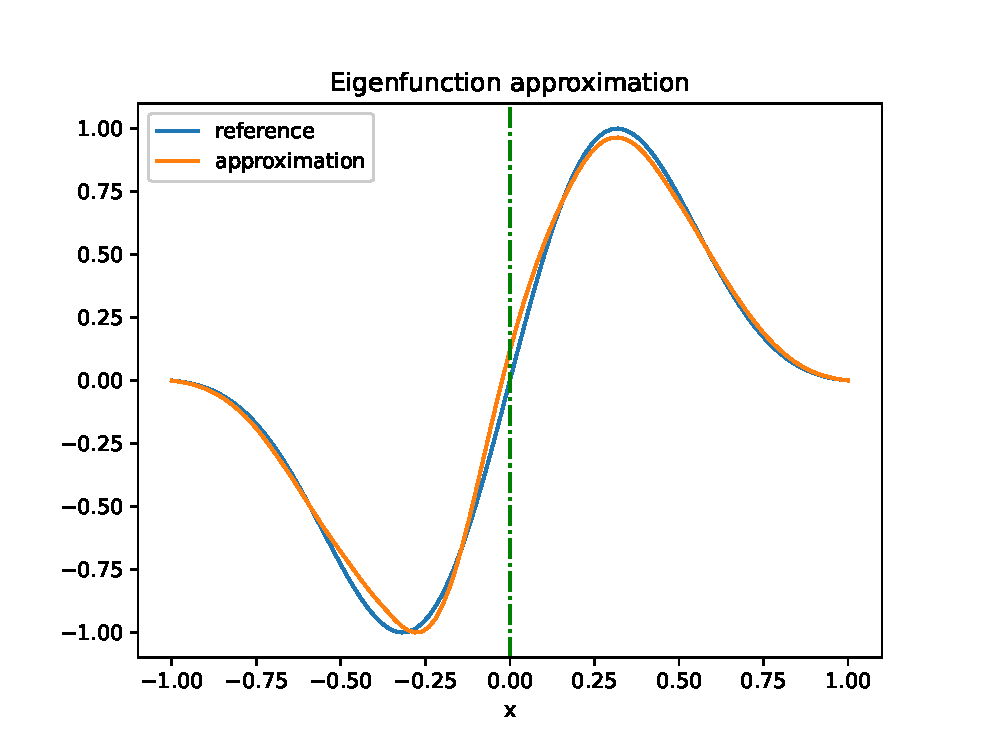
\includegraphics[width=\linewidth]{figures1/20d/unn_rank3.eps}
%         \caption{单位球上的 $\widehat{\xi}_{\phi 3}$}
%         \label{fig:xi_rank3}
%     \end{subfigure}
%     \hfill
%     \begin{subfigure}{0.48\textwidth}
%         \centering
%         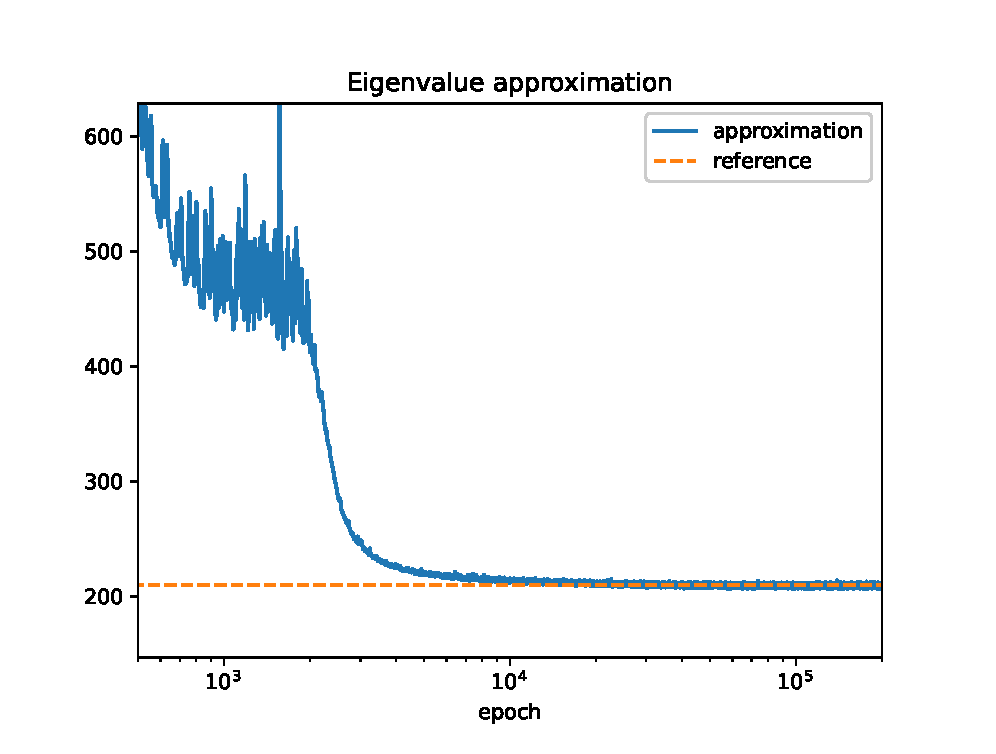
\includegraphics[width=\linewidth]{figures1/20d/eigenvalue_rank3.eps}
%         \caption{单位球上的 $\lambda_{3}$}
%         \label{fig:lambda_rank3}
%     \end{subfigure}
    
%     \caption{左列：20维单位球对角线上的特征函数。右列：特征值随训练轮次（Epoch）的演变情况。}
%     \label{fig:20dball}
% \end{figure}

\section{结论与讨论}\label{sec dis}
本文研究了利用神经网络求解椭圆多重特征值问题。我们基于椭圆特征值问题的惩罚变分形式，提出了一种计算椭圆多重特征值的通用形式。我们利用 Deep Ritz 方法求解了该惩罚变分形式。我们建立了估计特征值与真实特征值之间误差的上界，该上界与网络的深度 $\mathcal{D}$、宽度 $\mathcal{W}$ 以及训练样本量 $n$ 有关。通过探讨特征值问题的正则性并适当选择深度 $\mathcal{D}$ 和宽度 $\mathcal{W}$，我们表明该误差界克服了维数灾难。若干模拟结果证明了所提方法的有效性，并支持了我们的理论结果。

\section{附录}\label{app:proofingen}
\subsection{引理 \ref{lemma:staerr:Rad234} 的证明}
\begin{proof}[引理 \ref{lemma:staerr:Rad234}]\label{pf:lemma:staerr:Rad234}

引理的证明可分为两部分。我们首先证明后四个不等式，这主要依赖于 Rademacher 复杂度的 Lipschitz 收缩不等式：
\begin{lemma}\label{lemma:staerr:liprad}
假设函数 $\psi:\mathbb{R}^{d}\times\mathbb{R}\rightarrow\mathbb{R}$ 满足 $(x,y)\mapsto\psi(x,y)$，且对任意给定的 $x$，其关于 $y$ 是 $\ell$-Lipschitz 连续的。令 $\mathcal{N}$ 为定义在 $\Omega$ 上的函数类，并记 $\psi\circ\mathcal{N}=\{\psi\circ u:x\mapsto\psi(x,u(x)), u\in\mathcal{N}\}$，则有：
$$ \mathfrak{R}(\psi\circ\mathcal{N})\leq\ell \ \mathfrak{R}(\mathcal{N}). $$
\end{lemma}
该引理的严谨推导可参见文献 \cite{ledoux2013probability} 中的推论 3.17。基于此推论，对于引理\ref{lemma:staerr:Rad234}的第二个不等式，由于此情形下的 Lipschitz 常数为 $2\mathcal{B}^{2}$，我们可得：
$$ \sup _{u \in \mathcal{N}^{2}}\left|\mathcal{L}_{k, 2}(u)-\widehat{\mathcal{L}}_{k, 2}(u)\right| \leq |\Omega|\mathfrak{R}\left(\left\{w u^{2}:u\in \mathcal{N}^{2}\right\}\right) \leq 2|\Omega|\mathcal{B}^{2}\mathfrak{R}\left(\mathcal{N}^{2}\right). $$

同理，第三个不等式亦可由此得出，其对应的 Lipschitz 常数为 $2\mathcal{B}$。

至于最后两个不等式，我们使用如下不等式： 
\begin{equation*} 
|a^{2}-b^{2}|\leq 2|a||a-b|+|a-b|^{2}. 
\end{equation*}
利用类似的方法即可推导得出相应结论。

接下来，我们单独处理第一个不等式。由于梯度算子 $\nabla$ 不具备 Lipschitz 连续性，无法直接应用引理 \ref{lemma:staerr:liprad}。为此，我们需要证明 $\nabla u$ 的平方项（即 $|\nabla u|^2$）可由 $\mathrm{ReLU}$-$\mathrm{ReLU}^{2}$ 混合网络实现。具体而言，受 Baur-Strassen 关于多项式及其偏导数计算复杂度的理论启发 \cite{baur1983complexity}，我们提出如下引理：

\begin{lemma}
设 $u$ 为由深度 $\mathcal{D}$、宽度 $\mathcal{W}$ 的 $\mathrm{ReLU}^{2}$ 神经网络所实现的函数，则其梯度的平方项 $|\nabla u|^2$ 可由一个深度不超过 $2\mathcal{D}$、宽度不超过 $(2\mathcal{D}+4)\mathcal{W} + 2d$ 的 $\mathrm{ReLU}$-$\mathrm{ReLU}^{2}$ 混合网络精确表示。
\end{lemma}

\begin{proof}
为表述简便，下文将 $\mathrm{ReLU}$ 与 $\mathrm{ReLU}^{2}$ 激活函数分别记为 $\sigma_1$ 与 $\sigma_2$。容易观察到导数关系 $\sigma_2'(x)=2\sigma_1(x)$。我们将通过构造法来证明本引理。沿用定义 \ref{def:fnn} 中的记号，设 $u^{(k)}$ 为原 $\mathrm{ReLU}^{2}$ 网络第 $k$ 层的激活值，令 $z^{(k)} = W^{(k)}u^{(k-1)} + b^{(k)}$，且 $u^{(k)}=\sigma_2(z^{(k)})$。不失一般性，假设原网络具有单神经元线性输出，即 $u = z_1^{(\mathcal{D})}$。整个构造过程可划分为以下三个阶段：

首先，我们利用 $\mathrm{ReLU}$-$\mathrm{ReLU}^{2}$ 网络重现原网络的前向计算，并同时记录反向推导所需的全部局部导数。记第 $k$ 层的局部导数为 $c^{(k)}$，则有：
$$c^{(k)} = \sigma_2'(z^{(k)}) = 2\sigma_1(z^{(k)})$$
利用 $\sigma_1$ 函数的性质，恒等映射可精确表示为 $x = \sigma_1(x) - \sigma_1(-x)$。因此，在网络传播过程中传递并保留这些局部导数只需使用 $\sigma_1$ 激活函数。为了完整复现原网络的计算并缓存所有局部导数，此阶段需要深度 $\mathcal{D}$。在计算第 $k$ 层时，计算激活值 $u^{(k)}$ 至多消耗 $\mathcal{W}$ 个神经元，而缓存前 $k$ 层的局部导数至多消耗 $2k\mathcal{W}$ 个神经元。由此可知，该阶段的最大宽度受限于 $\mathcal{W} + 2\mathcal{D}\mathcal{W} = (2\mathcal{D}+1)\mathcal{W}$。

第二步，计算伴随变量，这里伴随变量定义为网络输出对各层预激活值的梯度，即 $\delta^{(k)} = \nabla_{z^{(k)}} u$。初始化 $\delta^{(\mathcal{D})} = 1$。根据多元微积分的链式法则，可得如下反向递推关系：
$$\delta_q^{(k)} = c_q^{(k)} \cdot \sum_{p=1}^{n_{k+1}} W_{pq}^{(k+1)} \delta_p^{(k+1)}$$
令 $v_q^{(k)} = \sum_{p=1}^{n_{k+1}} W_{pq}^{(k+1)} \delta_p^{(k+1)}$。注意到 $v_q^{(k)}$ 仅为第 $k+1$ 层伴随变量的线性组合，无需消耗额外的非线性计算深度。利用极化恒等式（$xy=\frac{1}{4}\left[(x+y)^2-(x-y)^2\right]$），两个标量 $c_q^{(k)}$ 与 $v_q^{(k)}$ 的乘法操作可通过一个单隐藏层内包含 $4$ 个 $\sigma_2$ 神经元的子网络精确实现：
$$c_q^{(k)} \cdot v_q^{(k)} = \frac{1}{4}\left[\sigma_2(c_q^{(k)}+v_q^{(k)}) + \sigma_2(-c_q^{(k)}-v_q^{(k)}) - \sigma_2(c_q^{(k)}-v_q^{(k)}) - \sigma_2(-c_q^{(k)}+v_q^{(k)})\right]$$
我们将原网络的计算图进行反向展开，针对 $k$ 从 $\mathcal{D}-1$ 递减至 $1$，逐层构造上述乘法子网络以计算 $\delta^{(k)}$。由于 $c_q^{(k)}$ 和 $v_q^{(k)}$ 均可由已有的网络节点通过线性组合获得，每次计算 $\delta^{(k)}$ 仅需通过 $1$ 层 $\sigma_2$ 激活函数。该反向递推共需进行 $\mathcal{D}-1$ 次，因此本阶段消耗的深度为 $\mathcal{D}-1$。在每层中，至多需要并行计算 $\mathcal{W}$ 个乘法，消耗 $4\mathcal{W}$ 个神经元。同时，网络需要继续向下层传递剩余未使用的缓存变量 $c^{(1)}, \dots, c^{(k-1)}$，这部分占用至多 $2(\mathcal{D}-1)\mathcal{W}$ 个神经元。因此，此阶段的最大宽度界限为 $4\mathcal{W} + 2\mathcal{D}\mathcal{W}$

第三步，计算梯度并平方求和：当递推至第一层并获得 $\delta^{(1)}$ 后，即可一次性求出针对所有 $d$ 个输入变量的偏导数：
$$\partial_i u = \sum_{p=1}^{n_1} W_{pi}^{(1)} \delta_p^{(1)}, \quad i=1, 2, \dots, d$$
最后，计算梯度向量模长的平方：
$$|\nabla u|^2 = \sum_{i=1}^d (D_i u)^2 = \sum_{i=1}^d \left[ \sigma_2(D_i u) + \sigma_2(-D_i u) \right]$$
由于求偏导数 $D_iu$ 属于线性映射，最终的平方与求和操作只需增加 $1$ 层 $\sigma_2$ 非线性层。在此最终层内，需并行计算 $d$ 个维度分量的平方展开项，共消耗 $2d$ 个神经元。

将上述三个阶段级联，所构造的目标混合网络的总复杂度受限于：
\begin{itemize}
    \item 总深度： $\mathcal{D}\left(|\nabla u|^2\right) = \mathcal{D} + (\mathcal{D}-1) + 1 = 2\mathcal{D}$
    \item 总宽度： 取各计算阶段宽度的最大值：
    $$\mathcal{W}\left(|\nabla u|^2\right) \leq \max\left\{ (2\mathcal{D}+1)\mathcal{W}, \ 2d \right\} \leq (2\mathcal{D}+4)\mathcal{W} + 2d$$
\end{itemize}


\end{proof}

\end{proof}

\subsection{引理 \ref{lemma:staerr:Rad_cover} 的证明}
\begin{proof}[引理 \ref{lemma:staerr:Rad_cover}]\label{pf:lemma:staerr:Rad_cover}
首先，我们引入 Massart 有限类引理（Massart's finite class lemma），其详细证明可参阅文献 \cite{boucheron2013concentration}。

\begin{lemma}[Massart 有限类引理 \cite{boucheron2013concentration}]\label{Mfinite}
对于任意给定的有限集 $V\subset\mathbb{R}^{n}$，记其最大向量 $\ell_2$ 范数为 $D=\sup_{v\in V}\|v\|_{2}$。则有：
$$ \mathbb{E}_{\Sigma_{n}}\left[ \sup_{v\in V}\frac{1}{n}\left| \sum_{i=1}^{n}\sigma_{i}v_{i} \right| \right] \leq \frac{D}{n}\sqrt{2\log(2|V|)}, $$
其中 $\sigma_{i}$ 和 $\mathbb{E}_{\Sigma_{n}}$ 分别为定义 \ref{def:staerr:radcom} 中所述的 Rademacher 随机变量及其期望。
\end{lemma}
接下来，我们采用标准的链式推导（Chaining Method）。令 $\varepsilon_{k}=2^{-k+1} B$。记 $\mathcal{F}_{k}$ 为 $\mathcal{F}$ 在无穷范数下的一个 $\varepsilon_{k}$-覆盖集，其基数满足 $\left|\mathcal{F}_{k}\right|=\mathcal{C}\left(\varepsilon_{k}, \mathcal{F},\|\cdot\|_{\infty}\right)$。这意味着，对于任意函数 $u \in \mathcal{F}$，必定存在 $u_{k} \in \mathcal{F}_{k}$ 使得 $\left\|u-u_{k}\right\|_{\infty} \leq \varepsilon_{k}$。令 $K$ 为一个待定的正整数。通过项的分解与三角不等式，我们有：

$$ \begin{aligned} 
    &\quad\; \mathbb{E}_{\left\{\sigma_{i}, Z_{i}\right\}_{i=1}^{n}}\left[\sup\limits_{u \in \mathcal{F}} \frac{1}{n}\left|\sum\limits_{i=1}^{n} \sigma_{i} u\left(Z_{i}\right)\right|\right] \\ &= \mathbb{E}_{\left\{\sigma_{i}, Z_{i}\right\}_{i=1}^{n}}\left[\sup\limits _{u \in \mathcal{F}} \frac{1}{n}\left|\sum\limits_{i=1}^{n} \sigma_{i}\left(u\left(Z_{i}\right)-u_{K}\left(Z_{i}\right)\right) + \sum\limits_{j=1}^{K-1} \sum\limits_{i=1}^{n} \sigma_{i}\left(u_{j+1}\left(Z_{i}\right)-u_{j}\left(Z_{i}\right)\right) + \sum\limits_{i=1}^{n} \sigma_{i} u_{1}\left(Z_{i}\right)\right|\right] \\ &\leq \mathbb{E}_{\left\{\sigma_{i}, Z_{i}\right\}_{i=1}^{n}}\left[\sup\limits _{u \in \mathcal{F}} \frac{1}{n}\left|\sum\limits_{i=1}^{n} \sigma_{i}\left(u\left(Z_{i}\right)-u_{K}\left(Z_{i}\right)\right)\right|\right] \\ &\quad + \sum\limits_{j=1}^{K-1} \mathbb{E}_{\left\{\sigma_{i}, Z_{i}\right\}_{i=1}^{n}}\left[\sup\limits _{u \in \mathcal{F}} \frac{1}{n}\left|\sum\limits_{i=1}^{n} \sigma_{i}\left(u_{j+1}\left(Z_{i}\right)-u_{j}\left(Z_{i}\right)\right)\right|\right] \\ &\quad + \mathbb{E}_{\left\{\sigma_{i}, Z_{i}\right\}_{i=1}^{n}}\left[\sup\limits _{u \in \mathcal{F}} \frac{1}{n}\left|\sum\limits_{i=1}^{n} \sigma_{i} u_{1}\left(Z_{i}\right)\right|\right]. 
\end{aligned} $$
由于零函数 $0 \in \mathcal{F}$，我们可以无妨设定 $\mathcal{F}_{1}=\{0\}$，从而消除上述不等式中的第三项。对于第一项，应用 Rademacher 变量的性质与 Hölder 不等式：
\begin{equation*}
\begin{aligned}
{}&\mathbb{E}_{\left\{\sigma_{i}, Z_{i}\right\}_{t=1}^{n}}\left[\sup\limits _{u \in \mathcal{F}} \frac{1}{n}\left|\sum\limits_{i=1}^{n} \sigma_{i}\left(u\left(Z_{i}\right)-u_{K}\left(Z_{i}\right)\right)\right|\right]\\
\leq&\mathbb{E}_{\left\{\sigma_{i}, Z_{i}\right\}_{i=1}^{n}}\left[\sup\limits _{u \in \mathcal{F}} \frac{1}{n} \sum\limits_{i=1}^{n}\left|\sigma_{i}\right|\left\|u-u_{K}\right\|_{\infty}\right] \leq \varepsilon_{K}
\end{aligned}
\end{equation*}
对于第二项中的求和单元，定义向量 $v_{i}^{j}=u_{j+1}\left(Z_{i}\right)-u_{j}\left(Z_{i}\right)$，并应用引理 \ref{Mfinite}，得到：
\begin{equation*}
\begin{aligned}
&\sum_{j=1}^{K-1} \mathbb{E}_{\{\sigma\}_{i=1}^{n}}\left[\sup _{u \in \mathcal{F}} \frac{1}{n}\left|\sum_{i=1}^{n} \sigma_{i}\left(u_{j+1}\left(Z_{i}\right)-u_{j}\left(Z_{i}\right)\right)\right|\right]\\
=&\sum_{j=1}^{K-1} \mathbb{E}_{\left\{\sigma_{t}\right\}_{t=1}^{n}}\left[\sup _{v \in V_{j}} \frac{1}{n} \left| \sum_{i=1}^{n} \sigma_{i} v_{i}^{j}\right|\right] \leq \sum_{j=1}^{K-1} \frac{D_{j}}{n} \sqrt{2 \log \left(2\left|V_{j}\right|\right)}.
\end{aligned}
\end{equation*}
根据集合 $V_{j}$ 的构造，其势满足界限 $\left|V_{j}\right| \leq\left|\mathcal{F}_{j}\right|\left|\mathcal{F}_{j+1}\right| \leq\left|\mathcal{F}_{j+1}\right|^{2}$。同时，向量的范数上界 $D_j$ 可被限制为：
$$ \begin{aligned}
     D_j &= \sup_{v \in V_j} \left(\sum_{i=1}^{n}\left|u_{j+1}\left(Z_{i}\right)-u_{j}\left(Z_{i}\right)\right|^{2}\right)^{1 / 2} \leq \sqrt{n}\left\|u_{j+1}-u_{j}\right\|_{\infty} \\ &\leq \sqrt{n}\left\|u_{j+1}-u\right\|_{\infty}+\sqrt{n}\left\|u_{j}-u\right\|_{\infty} = \sqrt{n} \varepsilon_{j+1}+\sqrt{n} \varepsilon_{j} = 3 \sqrt{n} \varepsilon_{j+1}. 
\end{aligned} $$
将其代入前式，有：
\begin{equation*}
\begin{aligned}
&\sum_{j=1}^{K-1} \mathbb{E}_{\left\{\sigma_{i}, Z_{t}\right\}_{t=1}^{n}}\left[\sup _{u \in \mathcal{F}} \frac{1}{n}\left|\sum_{i=1}^{n} \sigma_{i}\left(u_{j+1}\left(Z_{i}\right)-u_{j}\left(Z_{i}\right)\right)\right|\right] \\
&\leq \sum_{j=1}^{K-1} \frac{D_{j}}{n} \sqrt{2 \log \left(2\left|V_{j}\right|\right)} \leq \sum_{j=1}^{K-1} \frac{3 \varepsilon_{j+1}}{\sqrt{n}} \sqrt{2 \log \left(2\left|\mathcal{F}_{j+1}\right|^{2}\right)}
\end{aligned}
\end{equation*}
结合上述所有界的估计，我们将离散求和转化为 Dudley 积分形式：
\begin{equation*}
\begin{aligned}
&\mathbb{E}_{\left\{\sigma_{i}, Z_{i}\right\}_{i=1}^{n}}\left[\sup _{u \in \mathcal{F}} \frac{1}{n}\left|\sum_{i=1}^{n} \sigma_{i} u\left(Z_{i}\right)\right|\right] \leq \varepsilon_{K}+\sum_{j=1}^{K-1} \frac{6 \varepsilon_{j+2}}{\sqrt{n}} \sqrt{2 \log \left(2\left|\mathcal{F}_{j+1}\right|^{2}\right)} \\
&=\varepsilon_{K}+\frac{6}{\sqrt{n}} \sum_{j=1}^{K-1}\left(\varepsilon_{j+1}-\varepsilon_{j+2}\right) \sqrt{2 \log \left(2 \mathcal{C}\left(\varepsilon_{j+1}, \mathcal{F},\|\cdot\|_{\infty}\right)^{2}\right)}\\
&\leq \varepsilon_{K}+\frac{6}{\sqrt{n}} \int_{\varepsilon_{K+1}}^{B / 2} \sqrt{2 \log \left(2 \mathcal{C}\left(\varepsilon, \mathcal{F},\|\cdot\|_{\infty}\right)^{2}\right)} d \varepsilon.
\end{aligned}
\end{equation*}
最后，对于任意给定的精度 $0<\delta<\frac{B}{2}$，我们总可以通过选取充分大的 $K$ 使得 $\varepsilon_{K+2}<\delta \leq \varepsilon_{K+1}$，从而完成引理的证明。
\end{proof}

\subsection{引理 \ref{lemma:staerr:pdim} 的证明}
\begin{proof}[引理 \ref{lemma:staerr:pdim}]\label{pf:lemma:staerr:pdim}
本引理的证明思路如下：首先，我们回顾打散与 VC 维的严格定义。

为了估计多项式的 Pdim，我们引入以下引理（其详细证明见文献 \cite{anthony2009neural} 的定理 8.3）：

\begin{lemma}\label{lemma:covering_number}
设 $p_1,\cdots,p_m$ 为 $m$ 个具有 $n$ 个变量且最高次数不超过 $d$ 的多项式。若 $n \leq m$，则这些多项式符号组合的集合基数满足：
\begin{equation*}
|{(\operatorname{sign}(p_1(x)),\cdots,\operatorname{sign}(p_m(x))):x\in\mathbb{R}^n}| \leq 2\left(\frac{2emd}{n}\right)^n
\end{equation*}

\end{lemma}
接下来的论证借鉴了文献 \cite{bartlett2019nearly} 中定理 6 的分析框架。需要指出的是，由于 $\mathrm{VCdim}(\operatorname{sign}(\mathcal{N})) \leq \mathrm{Pdim}(\mathcal{N})$，此处推导出的结论比原定理略强。

我们构造一个新的示性函数族： 
\begin{equation*}
\mathcal{\widetilde{N}}={\widetilde{u}(x,y)=\operatorname{sign}(u(x)-y): u\in\mathcal{N}}
\end{equation*}

根据定义，显然有 $\mathrm{Pdim}(\mathcal{N}) \leq \mathrm{VCdim}(\widetilde{\mathcal{N}})$。因此，问题转化为界定 $\widetilde{\mathcal{N}}$ 的 VC 维。设 $\mathcal{M}$ 为实现 $\mathcal{N}$ 中函数的神经网络的参数（权重与偏置）总数。对于任意给定的点集 $\{x_i\}_{i=1}^{m}\subset X$ 和 $\{y_i\}_{i=1}^{m}\subset\mathbb{R}$，我们考察由网络参数 $a \in \mathbb{R}^{\mathcal{M}}$ 诱导的二分法（dichotomies）数量：
\begin{equation*}
K_{{x_i},{y_i}}(m):=|{(\operatorname{sign}(u(x_{1}, a)-y_1), \ldots, \operatorname{sign}(u(x_{m}, a)-y_m)): a \in \mathbb{R}^{\mathcal{M}}}|
\end{equation*}
由定义可知，$K_{\{x_i\},\{y_i\}}(m)$ 在所有可能的 $\{x_i\}_{i=1}^{m}$ 与 $\{y_i\}_{i=1}^{m}$ 上的上确界，即为函数族 $\widetilde{\mathcal{N}}$ 的增长函数（Growth function） $\mathcal{G}_{\widetilde{\mathcal{N}}}(m)$。

为了能够应用引理 \ref{lemma:covering_number}，我们需要将参数空间 $\mathbb{R}^{\mathcal{M}}$ 划分为若干子区域，使得在每一个子区域内，网络输出 $u(x_i,a)-y_i$ 关于参数 $a$ 均表现为无断点（breakpoints）的多项式。沿用文献 \cite{bartlett2019nearly} 中的划分策略，我们将参数空间划分为 $\{P_1,P_2,\cdots,P_N\}$，其中区域总数 $N$ 满足：
\begin{equation} \label{pdimb1}
N\leq\prod_{i=1}^{\mathcal{D}-1}2\left(\frac{2emk_i(1+(i-1)2^{i-1})}{\mathcal{M}i}\right)^{\mathcal{M}i}
\end{equation}
上式中，$k_i$ 表示神经网络第 $i$ 层的神经元数量，而 $\mathcal{M}_i$ 表示截至第 $i$ 层（包含第 $i$ 层）所有神经元输入的参数总数。基于此划分，二分法总数可由各子区域内的二分法数量之和控制：
\begin{equation} \label{pdimb2}
K_{{x_i},{y_i}}(m)\leq\sum_{i=1}^{N}|{(\operatorname{sign}(u(x_{1}, a)-y_1), \cdots, \operatorname{sign}(u(x_{m}, a)-y_m)): a\in P_i}|
\end{equation}

注意到在每个子区域 $P_i$ 内，$u(x_i,a)-y_i$ 是关于 $a$ 的多项式。如文献 \cite{bartlett2019nearly} 所证，该多项式的次数与其自身次数一致，且上界为 $1 + (\mathcal{D}-1)2^{\mathcal{D}-1}$。因此，直接应用引理 \ref{lemma:covering_number} 可得每个子区域的界：
\begin{align}
& |{(\operatorname{sign}(u(x_{1}, a)-y_1), \cdots, \operatorname{sign}(u(x_{m}, a)-y_m)): a\in P_i}|\nonumber \\
& \leq2\left(\frac{2em(1+(\mathcal{D}-1)2^{\mathcal{D}-1})}{\mathcal{M}{\mathcal{D}}}\right)^{\mathcal{M}{\mathcal{D}}}\label{pdimb3}.
\end{align}
将式 (\ref{pdimb1}) 和 (\ref{pdimb3}) 代入式 (\ref{pdimb2}) 中，可推导出：
\begin{equation*}
K_{{x_i},{y_i}}(m)\leq\prod_{i=1}^{\mathcal{D}}2\left(\frac{2emk_i(1+(i-1)2^{i-1})}{\mathcal{M}_i}\right)^{\mathcal{M}i}.
\end{equation*}
由于该上界对所有样本点集均一致成立，故增长函数满足：
\begin{equation*}
\mathcal{G}_{\widetilde{\mathcal{N}}}(m)\leq\prod_{i=1}^{\mathcal{D}}2\left(\frac{2emk_i(1+(i-1)2^{i-1})}{\mathcal{M}_i}\right)^{\mathcal{M}_i},
\end{equation*}
最终，通过类似于文献 \cite{bartlett2019nearly} 中定理 6 的代数化简（令 $\mathcal{G}_{\widetilde{\mathcal{N}}}(m) < 2^m$ 并求解 $m$ 的界），我们可得：
\begin{equation*}
\mathrm{Pdim}(\mathcal{N})\lesssim C\left(\mathcal{D}^2\mathcal{W}^2 \log \mathcal{U}+\mathcal{D}^3\mathcal{W}^2\right)
\lesssim C\left(\mathcal{D}^2\mathcal{W}^2\left( \mathcal{D}+\log \mathcal{W}\right)\right)
\end{equation*}
其中常数 $C$ 与网络架构无关，$\mathcal{U}$ 为实现函数族 $\mathcal{N}$ 的神经网络中包含的神经元总数。至此，引理得证。
\end{proof}



%%%%==========================================================%%%
